% This template is created by SV Bùi Vân Anh, và Thầy Nguyễn Tiến Hòa từ phòng Lab xử lý tín hiệu băng gốc hệ thống 5G. Chúng tôi rất vui nếu được nhắc đến trong lời cảm ơn.
%%%%%%%%%%%%%%%%%%%%%%%%%%%%%%%%%%%%%%%%%%%%%%%%%%%%%%%
\documentclass{article} % Tạo một bản báo cáo
\usepackage[utf8]{inputenc}
\usepackage[T5]{fontenc} % Để sử dụng Tiếng Việt
\usepackage[fontsize=13pt]{scrextend} % Set fontsize=13pt
\usepackage[paperheight=29.7cm,paperwidth=21cm,right=2cm,left=3cm,top=2cm,bottom=2.5cm]{geometry}% Chuẩn A4, căn lề phải, trái, trên, dưới.
% \usepackage[paperheight=29.7cm,paperwidth=21cm,right=2cm,left=3cm,top=2cm,bottom=2.5cm,twoside]{geometry}% Chuẩn A4, căn lề phải, trái, trên, dưới.
\usepackage{mathptmx} % Time New Roman
\usepackage{amsmath}
\usepackage{graphicx} % Thư viện chèn ảnh
\usepackage{float} % Set vị trí chèn ảnh
\usepackage{tikz} % Thư viện tạo khung bìa
\usetikzlibrary{calc,positioning,arrows.meta} % Thư viện tikz
\usepackage{indentfirst} % Thư viện thụt đầu dòng
\usepackage{booktabs} % To thicken table lines
\renewcommand{\baselinestretch}{1.2} % Giãn dòng 1.2
\setlength{\parskip}{6pt} % Spacing after
\setlength{\parindent}{1cm} % Set khoảng cách thụt đầu dòng mỗi đoạn
\usepackage{titlesec} % Thư viện để set up các kiểu chữ
\setcounter{secnumdepth}{4} % 4 Heading
\titlespacing*{\section}{0pt}{0pt}{30pt} % Heading 1
\titleformat*{\section}{\fontsize{16pt}{0pt}\selectfont \bfseries \centering}

\titlespacing*{\subsection}{0pt}{10pt}{0pt} % Heading 2
\titleformat*{\subsection}{\fontsize{14pt}{0pt}\selectfont \bfseries}

\titlespacing*{\subsubsection}{0pt}{10pt}{0pt} % Heading 3
\titleformat*{\subsubsection}{\fontsize{13pt}{0pt}\selectfont \bfseries \itshape}

\titlespacing*{\paragraph}{0pt}{10pt}{0pt} % Heading 4
\titleformat*{\paragraph}{\fontsize{13pt}{0pt}\selectfont \itshape}

\renewcommand{\figurename}{\fontsize{12pt}{0pt}\selectfont \bfseries Hình}
\renewcommand{\thefigure}{\thesection.\arabic{figure}}
\usepackage[font=bf]{caption}
\captionsetup[figure]{labelsep=space}

\renewcommand{\tablename}{\fontsize{12pt}{0pt}\selectfont \bfseries Bảng}
\renewcommand{\thetable}{\thesection.\arabic{table}}
\captionsetup[table]{labelsep=space}

\usepackage{tabularx}
\newcolumntype{s}{>{\hsize=.3\hsize}X}
\newcolumntype{y}{>{\hsize=.4\hsize}X}
\newcolumntype{d}{>{\hsize=.1\hsize}X}
\newcolumntype{a}{>{\hsize=1.1\hsize}X}
\newcolumntype{g}{>{\hsize=5\hsize}X}
\renewcommand{\tabularxcolumn}[1]{>{\small}m{#1}}

\renewcommand{\theequation}{\thesection.\arabic{equation}} % Thay đổi đánh số phương trình mặc định
\newtheorem{theorem}{Định lý}[section]
\newtheorem{defn}[theorem]{Định nghĩa}
\newtheorem{corollary}[theorem]{Hệ quả}
\newtheorem{lemma}[theorem]{Bổ đề}

\usepackage{lipsum} % Thư viện tạo chữ linh tinh.
\renewcommand{\contentsname}{MỤC LỤC}
\renewcommand{\listfigurename}{DANH MỤC HÌNH VẼ}
\renewcommand{\listtablename}{DANH MỤC BẢNG BIỂU}
\renewcommand{\refname}{TÀI LIỆU THAM KHẢO}

\usepackage[unicode]{hyperref}
\usepackage{colortbl}
\definecolor{LightCyan}{rgb}{0.88,1,1}
\usepackage{forloop}
\newcounter{loopcntr}
\newcommand{\rpt}[2][1]{\forloop{loopcntr}{0}{\value{loopcntr}<#1}{#2}}

\begin{document}

\graphicspath{{Images/}}

\begin{titlepage}
\begin{tikzpicture}[overlay,remember picture]
\draw [line width=3pt]
    ($ (current page.north west) + (3.0cm,-2.0cm) $)
    rectangle
    ($ (current page.south east) + (-2.0cm,2.5cm) $);
\draw [line width=0.5pt]
    ($ (current page.north west) + (3.1cm,-2.1cm) $)
    rectangle
    ($ (current page.south east) + (-2.1cm,2.6cm) $); 
\end{tikzpicture}
\begin{center}
\vspace{-12pt}   TRƯỜNG ĐẠI HỌC VINUNI \\
\textbf{\fontsize{16pt}{0pt}\selectfont CÔNG TY VINSMART FUTURE}
\vspace{0.5cm}
 \begin{figure}[H]
     \centering
     
\includegraphics[width=5cm]{Images/VSF_logo.jpg}
 \end{figure}
\fontsize{24pt}{0pt}\selectfont BÁO CÁO \\
\vspace{12pt}
\textbf{\fontsize{32pt}{0pt}\selectfont THỰC TẬP DOANH NGHIỆP}
\vspace{1.5cm}
\end{center}

\begin{center}
    \hspace{6pt}\textbf{\fontsize{18pt}{0pt}\selectfont Đề tài:}\\
    \textbf{\fontsize{20pt}{0pt}\selectfont XÂY DỰNG HỆ THỐNG}\\
    \textbf{\fontsize{20pt}{0pt}\selectfont MULTI CAMERA TRACKING}

\vspace{1.5cm}
\begin{table}[H]
    \centering
    \begin{tabular}{l l}
 \fontsize{14pt}{0pt}\selectfont Sinh viên thực hiện:    & \fontsize{14pt}{0pt}\selectfont NGUYỄN LÊ TRUNG \vspace{6pt} \\ 
\fontsize{14pt}{0pt}\selectfont Mã số sinh viên:   &\fontsize{14pt}{0pt}\selectfont 2A202600174 \vspace{6pt}\\
\fontsize{14pt}{0pt}\selectfont Người hướng dẫn: & \fontsize{14pt}{0pt}\selectfont LÊ VŨ ĐỨC HƯNG
\end{tabular}
\end{table}
\vspace{3.5cm}
 \fontsize{14pt}{0pt}\selectfont Hà Nội, \today
\end{center}
\end{titlepage}

\cleardoublepage
\thispagestyle{empty}
\begin{tikzpicture}[overlay,remember picture]
\draw [line width=3pt]
    ($ (current page.north west) + (3.0cm,-2.0cm) $)
    rectangle
    ($ (current page.south east) + (-2.0cm,2.5cm) $);
\draw [line width=0.5pt]
    ($ (current page.north west) + (3.1cm,-2.1cm) $)
    rectangle
    ($ (current page.south east) + (-2.1cm,2.6cm) $); 
\end{tikzpicture}
\begin{center}
\vspace{-12pt}  TRƯỜNG ĐẠI HỌC VINUNI \\
\textbf{\fontsize{16pt}{0pt}\selectfont CÔNG TY VINSMART FUTURE}
\vspace{0.5cm}
 \begin{figure}[H]
     \centering
     
\includegraphics[width=5cm]{Images/VSF_logo.jpg}
 \end{figure}
\fontsize{24pt}{0pt}\selectfont BÁO CÁO \\
\vspace{12pt}
\textbf{\fontsize{32pt}{0pt}\selectfont THỰC TẬP DOANH NGHIỆP}
\vspace{1.5cm}
\end{center}

\begin{center}
    \hspace{6pt}\textbf{\fontsize{18pt}{0pt}\selectfont Đề tài:}\\
    \textbf{\fontsize{20pt}{0pt}\selectfont XÂY DỰNG HỆ THỐNG}\\
    \textbf{\fontsize{20pt}{0pt}\selectfont MULTI CAMERA TRACKING}

\vspace{1.5cm}
\begin{table}[H]
    \centering
    \begin{tabular}{l l}
 \fontsize{14pt}{0pt}\selectfont Sinh viên thực hiện:    & \fontsize{14pt}{0pt}\selectfont NGUYỄN LÊ TRUNG \vspace{6pt} \\ 
\fontsize{14pt}{0pt}\selectfont Mã số sinh viên:   &\fontsize{14pt}{0pt}\selectfont 2A202600174 \vspace{6pt}\\
\fontsize{14pt}{0pt}\selectfont Người hướng dẫn: & \fontsize{14pt}{0pt}\selectfont LÊ VŨ ĐỨC HƯNG
\end{tabular}
\end{table}
\vspace{2.5cm}
 \fontsize{14pt}{0pt}\selectfont Hà Nội, \today
\end{center}
\cleardoublepage % Bìa dự án.

\section*{LỜI NÓI ĐẦU}
\thispagestyle{empty}

Sự phát triển nhanh chóng của các hệ thống camera quan sát trong không gian công cộng và thương mại đặt ra nhu cầu cấp thiết về khả năng phân tích hành vi người tự động và theo thời gian thực. Việc theo dõi người qua nhiều camera --- duy trì danh tính nhất quán cho từng cá nhân khi họ di chuyển từ trường nhìn của camera này sang camera khác --- là bước tiên quyết để xây dựng các ứng dụng quản lý không gian thông minh như phân tích mật độ, đo lường thời gian dừng, tối ưu lưu lượng người, và hỗ trợ an ninh.

Dự án này được thực hiện trong khuôn khổ thực tập tại Công ty VinSmart Future dưới sự hướng dẫn của anh \textbf{Lê Vũ Đức Hưng}. Nhiệm vụ được giao là nghiên cứu và xây dựng một hệ thống theo dõi người đa camera (Multi-Camera Tracking) có khả năng hoạt động theo thời gian thực trên phần cứng GPU phổ thông, đồng thời cung cấp bộ công cụ phân tích mật độ không gian (heatmap) phục vụ phân tích lưu lượng người, giám sát an toàn và tối ưu bố trí không gian.

Trong suốt quá trình thực hiện, em đã nghiên cứu các công trình khoa học liên quan, tiến hành thực nghiệm trên bộ dữ liệu MMPTrack --- một bộ dữ liệu chuẩn cho bài toán này --- và từng bước xây dựng pipeline hoàn chỉnh từ phát hiện người, theo dõi cục bộ, nhận dạng lại xuyên camera, đến trực quan hóa kết quả và cung cấp số liệu phân tích.

Em xin trân trọng cảm ơn anh \textbf{Lê Vũ Đức Hưng} đã tận tình hướng dẫn, góp ý và hỗ trợ trong suốt thời gian thực hiện dự án. Em
 cũng xin cảm ơn Trường Đại học VinUni và Công ty VinSmart Future đã tạo điều kiện thuận lợi về cơ sở vật chất và môi trường làm việc.

\vspace{12pt}
\hspace{8cm}Hà Nội, \today

\hspace{8.5cm}\textbf{Sinh viên thực hiện}

\vspace{2cm}
\hspace{8.3cm}\textbf{NGUYỄN LÊ TRUNG}
\cleardoublepage
 % Lời nói đầu.

 % Tạo mục lục tự động
\addtocontents{toc}{\protect\thispagestyle{empty}}
\tableofcontents
\thispagestyle{empty}
\clearpage

\pagenumbering{roman}
\section*{DANH MỤC CHỮ VIẾT TẮT}
\phantomsection\addcontentsline{toc}{section}{\numberline {}DANH MỤC CHỮ VIẾT TẮT}

\begin{table}[H]
\centering
\begin{tabular}{p{3.2cm} p{13cm}}
\toprule
\textbf{Viết tắt} & \textbf{Giải thích} \\
\midrule
API      & Application Programming Interface (giao diện lập trình ứng dụng) \\
BEV      & Bird's-Eye View (góc nhìn từ trên xuống) \\
CC       & Correlation Coefficient (hệ số tương quan Pearson) \\
CUDA     & Compute Unified Device Architecture (nền tảng tính toán song song GPU của NVIDIA) \\
FP16     & Floating-Point 16-bit (độ chính xác thực dấu phẩy động 16 bit) \\
FP32     & Floating-Point 32-bit (độ chính xác thực dấu phẩy động 32 bit) \\
FPS      & Frames Per Second (khung hình mỗi giây) \\
GID      & Global Identity (định danh xuyên camera toàn cục) \\
GPU      & Graphics Processing Unit (đơn vị xử lý đồ họa) \\
HOTA     & Higher Order Tracking Accuracy (độ đo theo dõi bậc cao) \\
IDF1     & Identity F1 Score (điểm F1 định danh) \\
MCT      & Multi-Camera Tracking (theo dõi đa camera) \\
MOTA     & Multiple Object Tracking Accuracy (độ chính xác theo dõi đa đối tượng) \\
MOTP     & Multiple Object Tracking Precision (độ chính xác vị trí theo dõi đa đối tượng) \\
MOT      & Multiple Object Tracking (theo dõi đa đối tượng) \\
MTMC     & Multi-Target Multi-Camera (đa đối tượng đa camera) \\
NvDCF    & NVIDIA Discriminative Correlation Filter (bộ theo dõi lọc tương quan phân biệt) \\
ONNX     & Open Neural Network Exchange (định dạng mô hình mạng nơ-ron mở) \\
ReID     & Re-Identification (nhận dạng lại người) \\
ROI      & Region of Interest (vùng quan tâm) \\
SCT      & Single-Camera Tracking (theo dõi đơn camera) \\
SDK      & Software Development Kit (bộ công cụ phát triển phần mềm) \\
SGIE     & Secondary GPU Inference Engine (bộ suy luận GPU phụ trong DeepStream) \\
TensorRT & Tensor Runtime (thư viện tối ưu hóa suy luận sâu của NVIDIA) \\
VRAM     & Video Random Access Memory (bộ nhớ truy cập ngẫu nhiên video) \\
YOLO     & You Only Look Once (mô hình phát hiện đối tượng một lần duyệt) \\
\bottomrule
\end{tabular}
\end{table}

\newpage
 % Danh mục ký hiệu và chữ viết tắt

%Tạo danh mục hình vẽ.
{\let\oldnumberline\numberline
\renewcommand{\numberline}{Hình~\oldnumberline}
\listoffigures}
\phantomsection\addcontentsline{toc}{section}{\numberline {} DANH MỤC HÌNH VẼ}
\newpage

 %Tạo danh mục bảng biểu.
{\let\oldnumberline\numberline
\renewcommand{\numberline}{Bảng~\oldnumberline}
\listoftables}
\phantomsection\addcontentsline{toc}{section}{\numberline {} DANH MỤC BẢNG BIỂU}
\newpage

\section*{TÓM TẮT}
\phantomsection\addcontentsline{toc}{section}{\numberline {}TÓM TẮT}

Dự án trình bày quá trình xây dựng hệ thống theo dõi người theo thời gian thực trên mạng nhiều camera (Multi-Camera Tracking --- MCT), kết hợp bộ công cụ phân tích mật độ không gian phục vụ giám sát an toàn, phân tích lưu lượng người và tối ưu bố trí không gian. Hệ thống được kiểm thử trên bộ dữ liệu MMPTrack \cite{Han2022} gồm 5 môi trường, 23 camera và 28 đối tượng người khác nhau.

Hai mục tiêu kỹ thuật được đặt ra: (1) xử lý đồng thời 20 camera ở tốc độ tối thiểu 10 khung hình/giây/camera; (2) đạt độ chính xác định danh xuyên camera (Global IDF1) tối thiểu 0,8 trên tập kiểm thử với người chưa xuất hiện trong quá trình huấn luyện.

Hệ thống được triển khai trên nền tảng NVIDIA DeepStream 9.0 theo kiến trúc hai tầng. Tầng per-camera phát hiện người bằng YOLO11n fine-tune (mAP50 = 0,97), theo dõi cục bộ bằng bộ theo dõi NvDCF chế độ Legacy DCF, và trích xuất đặc trưng ngoại hình bằng mạng Swin Transformer ReID. Tầng cross-camera hợp nhất định danh cục bộ từ nhiều camera thành Global ID ổn định thông qua bộ phận \textit{CrossCameraGalleryProbe}, hỗ trợ ràng buộc hình học và hai chế độ định danh: Live ID (gán tức thời, độ trễ bằng 0) và Buffered ID (gom cụm theo cửa sổ trượt 30 giây dựa trên thuật toán anchor-guided \cite{Huang2023}).

Chất lượng dữ liệu huấn luyện được nâng cao qua hai bước làm sạch nhãn: loại bỏ 17,6\% nhãn phantom trong tập phát hiện nhờ bộ kiểm tra độc lập COCO YOLO11x, và hợp nhất 196 nhãn scene-local về 56 identity sạch cho mô hình ReID, giúp khoảng cách val gap tăng từ 0,52 lên 0,87.

Hệ thống bổ sung ba loại bản đồ mật độ người: \textit{Occupancy} (tổng thời gian hiện diện), \textit{Footfall} (số người khác nhau đi qua), và \textit{Dwell-time} = Occupancy / Footfall theo Định luật Little \cite{Little1961}. Heatmap đạt hệ số tương quan (CC) từ 0,97 đến 0,99 so với nhãn thực trên tất cả các môi trường.

Kết quả thực nghiệm trên GPU RTX 5060 Ti (16GB): hệ thống đạt \textbf{$\sim$10{,}6 FPS/cam ở 20 camera đồng thời} (preset reid0) và \textbf{Global IDF1 trung bình 0,811} trên 5 môi trường kiểm thử (Lobby 0,895; Office 0,861; Café 0,833; Industry 0,805; Retail 0,660), vượt cả hai mục tiêu đề ra.

\cleardoublepage
 % Tóm tắt dự án

\pagenumbering{arabic} % Đánh số thứ tự 1,2,3...

%%%%%%%%%%%%%%%%%%%%%%%%%%%%%%%%%%%%%%%%%%%%%%%%%%
%               CHƯƠNG 1: GIỚI THIỆU
%%%%%%%%%%%%%%%%%%%%%%%%%%%%%%%%%%%%%%%%%%%%%%%%%%
\section*{CHƯƠNG 1.  GIỚI THIỆU}
\addcontentsline{toc}{section}{\numberline{}CHƯƠNG 1.  GIỚI THIỆU}
\setcounter{section}{1}
\setcounter{subsection}{0}
\setcounter{figure}{0}
\setcounter{table}{0}

\subsection{Đặt vấn đề}

Sự bùng nổ của các hệ thống camera quan sát trong không gian thương mại và công cộng --- từ cửa hàng bán lẻ, quán café, khu văn phòng đến khu công nghiệp và sảnh khách sạn --- tạo ra lượng dữ liệu hình ảnh khổng lồ nhưng phần lớn chỉ được dùng để xem lại sau sự cố, thay vì khai thác thời gian thực cho mục đích quản lý không gian.

Một trong những bài toán có giá trị thực tiễn cao nhất là \textit{theo dõi người đa camera} (Multi-Camera Tracking --- MCT): duy trì định danh nhất quán cho từng cá nhân khi họ di chuyển qua nhiều trường nhìn của các camera khác nhau. Khả năng này là tiền đề để tính các chỉ số quản lý như: số lượng khách hàng duy nhất đi qua một khu vực (Footfall), tỷ lệ thời gian khu vực bị chiếm dụng (Occupancy), thời gian khách hàng dừng lại tại điểm trưng bày (Dwell-time), hoặc cảnh báo khi mật độ người vượt ngưỡng an toàn.

Thách thức kỹ thuật chính của bài toán MCT nằm ở hai khía cạnh: (1) \textit{độ chính xác định danh xuyên camera} --- người cùng cá nhân phải được nhận ra qua sự thay đổi góc nhìn, ánh sáng, trang phục và thời gian vắng mặt; (2) \textit{tốc độ xử lý thời gian thực} --- hệ thống phải đủ nhanh để xử lý đồng thời nhiều camera mà không tích lũy độ trễ. Trong bối cảnh triển khai thực tế với ngân sách phần cứng hạn chế (GPU phổ thông), hai yêu cầu này thường xung đột nhau.

Phần lớn các nghiên cứu học thuật giải quyết bài toán này bằng cách xử lý offline (không phải thời gian thực) hoặc sử dụng cụm máy chủ GPU cao cấp, khiến chúng khó triển khai trong môi trường thương mại thực tế. Dự án này nhắm đến khoảng trống đó: xây dựng một hệ thống MCT đáp ứng cả hai yêu cầu trên một GPU phổ thông.

\subsection{Mục tiêu đề tài}

Dự án đặt ra hai mục tiêu kỹ thuật cụ thể, đo lường được:

\begin{enumerate}
    \item \textbf{Tốc độ xử lý:} Hệ thống phải xử lý được ít nhất 20 camera video đồng thời ở tốc độ tối thiểu 10 FPS/camera (tổng cộng $\geq 200$ FPS) trên một GPU duy nhất.

    \item \textbf{Độ chính xác định danh:} Hệ thống phải đạt Global IDF1 $\geq 0{,}8$ trên tập kiểm thử của bộ dữ liệu MMPTrack \cite{Han2022}, với người chưa xuất hiện trong quá trình huấn luyện (\textit{unseen subjects}).
\end{enumerate}

Bên cạnh đó, dự án cũng hướng tới mục tiêu thứ cấp là cung cấp bộ công cụ phân tích không gian bổ sung (heatmap Occupancy, Footfall, Dwell-time) phục vụ phân tích sử dụng không gian trong nhiều ngữ cảnh khác nhau: quản lý an toàn, tối ưu bố cục, giám sát lưu lượng người.

\subsection{Đóng góp chính}

Dự án có bốn đóng góp kỹ thuật chính:

\begin{enumerate}
    \item \textbf{Pipeline thời gian thực trên DeepStream:} Hệ thống hai tầng --- per-camera tracking và cross-camera identity fusion --- chạy trên NVIDIA DeepStream 9.0, đạt $\sim$15 FPS/camera ở 20 camera đồng thời (preset reid0, \texttt{maxTargetsPerStream=40}).

    \item \textbf{Quy trình làm sạch nhãn:} Hai công cụ làm sạch nhãn độc lập cho YOLO (dùng bộ xác nhận COCO YOLO11x loại $\sim$42\% nhãn bị che khuất của riêng môi trường retail, nâng precision phát hiện từ 0,62 lên 0,94) và cho ReID (hợp nhất 196 nhãn scene-local về 56 identity sạch), giúp mô hình tổng quát hóa tốt hơn đáng kể sang người chưa thấy.

    \item \textbf{Buffered ID dựa trên anchor-guided clustering:} Triển khai thuật toán anchor-guided từ \cite{Huang2023} thành chế độ cửa sổ trượt 20 giây trong pipeline thời gian thực, đạt 97--98\% chất lượng của xử lý offline.

    \item \textbf{Heatmap phân tích mật độ:} Ba loại bản đồ mật độ (Occupancy, Footfall, Dwell-time) chuẩn hóa theo Định luật Little \cite{Little1961}, tích hợp trực tiếp vào pipeline.
\end{enumerate}

\subsection{Cấu trúc báo cáo}

Báo cáo được tổ chức thành bốn chương:

\begin{itemize}
    \item \textbf{Chương 2 --- Cơ sở lý thuyết:} Định nghĩa bài toán MTMC, các độ đo đánh giá, hai bộ dữ liệu MMPTrack và MTMC, các mô hình thành phần (YOLO11n, NvDCF, Swin ReID, DeepStream), và tổng quan các nghiên cứu liên quan.

    \item \textbf{Chương 3 --- Phương pháp:} Mô tả chi tiết kiến trúc hệ thống, cơ chế định danh xuyên camera, chế độ Buffered ID, quy trình làm sạch nhãn, phân tích mật độ người, và kiến trúc triển khai production với giao diện Web.

    \item \textbf{Chương 4 --- Thực nghiệm và kết quả:} Thiết lập thực nghiệm, kết quả theo dõi theo từng môi trường, phân tích throughput, độ chính xác heatmap, so sánh kiến trúc ReID, và trực quan hoá pipeline trên MTMC.

    \item \textbf{Kết luận:} Tóm tắt kết quả, nhận xét hạn chế, và đề xuất hướng phát triển.
\end{itemize}

\newpage

%%%%%%%%%%%%%%%%%%%%%%%%%%%%%%%%%%%%%%%%%%%%%%%%%%
%               CHƯƠNG 2: CƠ SỞ LÝ THUYẾT
%%%%%%%%%%%%%%%%%%%%%%%%%%%%%%%%%%%%%%%%%%%%%%%%%%
\section*{CHƯƠNG 2.  CƠ SỞ LÝ THUYẾT}
\addcontentsline{toc}{section}{\numberline{}CHƯƠNG 2.  CƠ SỞ LÝ THUYẾT}
\setcounter{section}{2}
\setcounter{subsection}{0}
\setcounter{figure}{0}
\setcounter{table}{0}

\subsection{Bài toán theo dõi người đa camera}

\subsubsection{Định nghĩa bài toán}

Bài toán \textit{Multi-Target Multi-Camera Tracking} (MTMC) yêu cầu hệ thống đồng thời xử lý $N$ luồng video từ $N$ camera, phát hiện tất cả người xuất hiện trong mỗi khung hình, gán cho mỗi người một định danh cục bộ ổn định trong từng camera (Single-Camera Tracking --- SCT), và sau đó liên kết các định danh cục bộ từ các camera khác nhau thành \textit{Global ID} duy nhất và ổn định cho từng cá nhân.

Khác với bài toán SCT, MTMC phải giải quyết thêm các thách thức: (1) cùng một người có thể có ngoại hình rất khác nhau từ các góc camera khác nhau; (2) người có thể biến mất khỏi tất cả camera trong một khoảng thời gian dài; (3) hai người khác nhau có thể có ngoại hình tương tự (đặc biệt trong môi trường có đồng phục); (4) camera có thể có vùng chồng lắp hoặc không có vùng chồng lắp.

\subsubsection{Phân loại phương pháp tiếp cận}

Các phương pháp MTMC được phân thành hai nhóm chính:

\textbf{Late-fusion (hai giai đoạn):} Giai đoạn 1 thực hiện SCT độc lập trên mỗi camera để tạo ra các tracklet cục bộ. Giai đoạn 2 liên kết các tracklet từ nhiều camera dựa trên đặc trưng ngoại hình, vị trí không gian, và ràng buộc thời gian. Đây là hướng tiếp cận phổ biến nhất và phù hợp với yêu cầu thời gian thực vì hai giai đoạn có thể chạy song song.

\textbf{Early-fusion (một giai đoạn):} Các camera được xử lý đồng thời ngay từ đầu, thường thông qua không gian BEV (Bird's-Eye View) chung. Phương pháp này có thể loại bỏ ambiguity sớm hơn nhưng đòi hỏi hiệu chỉnh camera chính xác và chi phí tính toán cao hơn.

Dự án này thuộc nhóm late-fusion, phù hợp với pipeline streaming của DeepStream.

\subsection{Các độ đo đánh giá}

\subsubsection{Độ đo đơn camera: MOTA, MOTP và IDF1}

\textbf{MOTA} (Multiple Object Tracking Accuracy) đo lường tỷ lệ lỗi tổng hợp của tracker:
\begin{equation}
    \text{MOTA} = 1 - \frac{\text{FN} + \text{FP} + \text{IDSW}}{\text{GT}}
\end{equation}
trong đó FN là số lượng bỏ sót, FP là số phát hiện sai, IDSW là số lần chuyển đổi định danh, và GT là tổng số đối tượng thực.

\textbf{MOTP} (Multiple Object Tracking Precision) đo độ chính xác vị trí của các bounding box:
\begin{equation}
    \text{MOTP} = \frac{\sum_{t,i} d_{t,i}}{\sum_t c_t}
\end{equation}
trong đó $d_{t,i}$ là khoảng cách IoU giữa phát hiện và nhãn thực tại khung $t$, $c_t$ là số lượng ghép cặp đúng.

\textbf{IDF1} (Identity F1) là độ đo ưu tiên tính nhất quán định danh:
\begin{equation}
    \text{IDF1} = \frac{2 \cdot \text{IDTP}}{2 \cdot \text{IDTP} + \text{IDFP} + \text{IDFN}}
\end{equation}
trong đó IDTP là số bounding box được phát hiện đúng với đúng định danh, IDFP và IDFN là số bounding box sai định danh hoặc bỏ sót.

\subsubsection{Độ đo xuyên camera: Global IDF1}

Trong bài toán MTMC, \textbf{Global IDF1} được tính theo cùng công thức IDF1 nhưng áp dụng trên toàn bộ video từ tất cả các camera, với Global ID thay cho local track ID. Đây là độ đo chính của dự án vì nó trực tiếp phản ánh khả năng duy trì định danh nhất quán xuyên camera.

\subsection{Bộ dữ liệu MMPTrack}

MMPTrack \cite{Han2022} là bộ dữ liệu MTMC quy mô lớn được thu thập trong môi trường mô phỏng, bao gồm 5 môi trường: quán cafe (\textit{cafe}), sảnh lễ tân (\textit{lobby}), văn phòng (\textit{office}), khu công nghiệp (\textit{industry}) và cửa hàng bán lẻ (\textit{retail}). Đặc điểm bộ dữ liệu được trình bày trong Bảng~\ref{tab:mmp}; Hình~\ref{fig:mmp_envs} minh họa khung hình đại diện từ mỗi môi trường.

\begin{table}[H]
    \centering
    \caption[Đặc điểm bộ dữ liệu MMPTrack]{\bfseries\fontsize{12pt}{0pt}\selectfont Đặc điểm bộ dữ liệu MMPTrack \cite{Han2022}}
    \begin{tabular}{|l|c|}
    \hline
    \bfseries Đặc điểm & \bfseries Giá trị \\
    \hline
    Số môi trường & 5 \\
    Số camera & 23 \\
    Số đối tượng người & 28 \\
    Tổng số khung hình & $\sim$2{,}97 triệu \\
    Tổng thời lượng & 576 phút \\
    Tốc độ khung hình & 15 FPS \\
    Độ phân giải & 640$\times$360 \\
    \hline
    \end{tabular}
    \label{tab:mmp}
\end{table}

\begin{figure}[H]
    \centering
    \begin{minipage}[t]{0.32\textwidth}
        \centering
        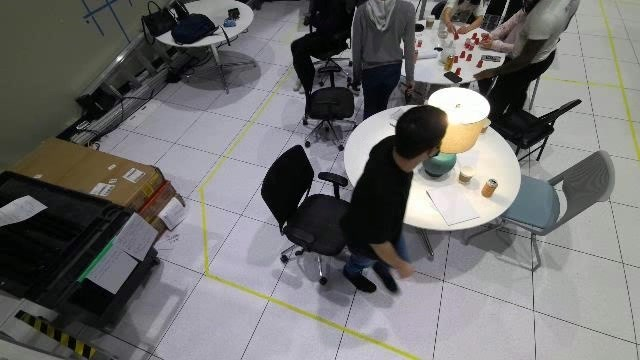
\includegraphics[width=\textwidth]{orig_cafe_shop_cam1}
        \small (a) Café
    \end{minipage}
    \hfill
    \begin{minipage}[t]{0.32\textwidth}
        \centering
        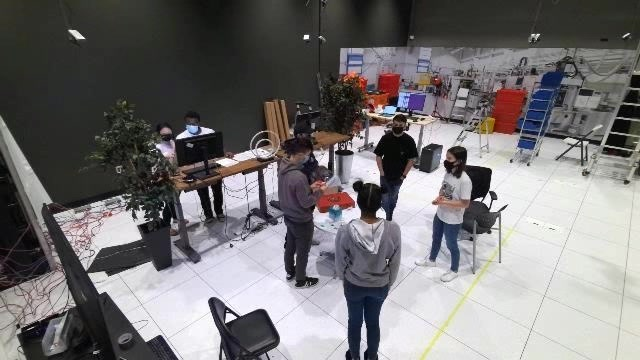
\includegraphics[width=\textwidth]{orig_lobby_cam1}
        \small (b) Lobby
    \end{minipage}
    \hfill
    \begin{minipage}[t]{0.32\textwidth}
        \centering
        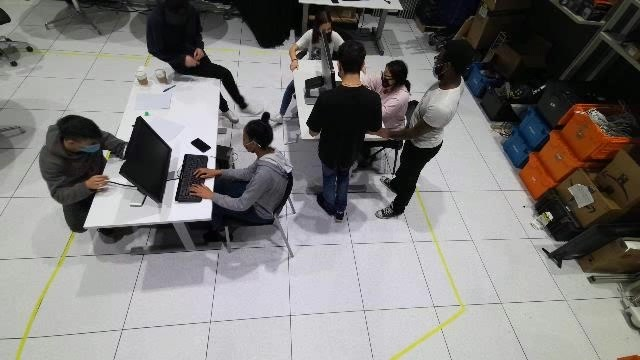
\includegraphics[width=\textwidth]{orig_office_cam1}
        \small (c) Office
    \end{minipage}
    \\[6pt]
    \begin{minipage}[t]{0.48\textwidth}
        \centering
        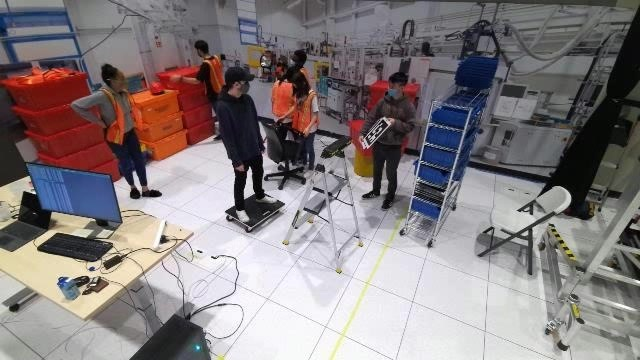
\includegraphics[width=\textwidth]{orig_industry_safety_cam1}
        \small (d) Industry
    \end{minipage}
    \hfill
    \begin{minipage}[t]{0.48\textwidth}
        \centering
        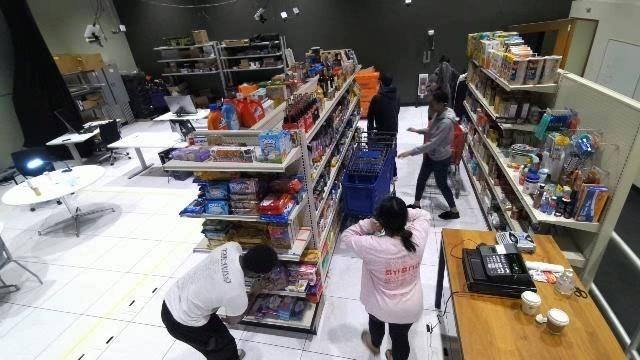
\includegraphics[width=\textwidth]{orig_retail_cam1}
        \small (e) Retail
    \end{minipage}
    \caption{Khung hình đại diện từ 5 môi trường trong bộ dữ liệu MMPTrack.}
    \label{fig:mmp_envs}
\end{figure}

Bộ dữ liệu được chia thành tập train và tập validation. Tập validation sử dụng trong dự án này là \textit{session 64pm} của MMPTrack, gồm 24 scene kiểm thử với người chưa xuất hiện trong tập train.

Một đặc điểm quan trọng của MMPTrack là nhãn \texttt{person\_id} được dán nhãn theo từng scene (\textit{scene-local}), không theo từng cá nhân thực. Điều này có nghĩa là cùng một người có thể có các \texttt{person\_id} khác nhau ở các scene khác nhau, gây ra nhiễu cho quá trình huấn luyện mô hình ReID --- vấn đề này được giải quyết chi tiết trong Phần~\ref{sec:label_cleaning}.

Phương pháp baseline được công bố trong bài báo gốc (DMCT-Ext-TD) đạt IDF1 = 74{,}1 trên tập validation \cite{Han2022}.

\subsection{Bộ dữ liệu MTMC}
\label{sec:mtmc_dataset}

Bên cạnh MMPTrack, dự án sử dụng thêm bộ dữ liệu MTMC\_Tracking\_2026 (sau đây gọi tắt MTMC) của cuộc thi NVIDIA AI City Challenge \cite{Tang25AICity25,Wang24AICity24}, theo dõi người đa camera trong môi trường kho hàng. MTMC được chọn vì phù hợp hơn để trực quan hoá các chức năng phân tích của pipeline: nhờ có hiệu chỉnh hình học metric, các camera trong kho được chiếu về một bản đồ tầm nhìn từ trên xuống (bird's-eye view --- BEV) chung, thuận tiện cho việc hiển thị heatmap mật độ và quỹ đạo theo dõi trên mặt bằng --- điều mà MMPTrack (không có calibration metric) không làm được. Quá trình chạy pipeline trên bối cảnh này đồng thời giúp bộc lộ một số hạn chế của phương pháp (Phần~\ref{sec:mtmc_results}). Vì đây là dữ liệu mô phỏng (không phải người thật), MTMC chỉ đóng vai trò trực quan hoá chức năng, không phải tập đánh giá định lượng; MMPTrack vẫn là tập đo IDF1 chuẩn. Trong phạm vi dự án, MTMC được dùng giới hạn ở một kho duy nhất là Warehouse\_022, và hai bộ dữ liệu được giữ tách biệt hoàn toàn (mô hình, cấu hình, mã đánh giá riêng).

MTMC khác MMPTrack ở ba điểm quyết định thiết kế thuật toán (Bảng~\ref{tab:mmp_vs_mtmc}): (1) camera rời rạc (disjoint FOV) --- mỗi người có thể chỉ xuất hiện ở một camera tại một thời điểm, nên bài toán cốt lõi là bàn giao (hand-off) danh tính khi người di chuyển giữa các vùng camera, ngược với FOV chồng lấn của MMP; (2) có \texttt{calibration.json} metric (ma trận nội $K$ + ngoại $[R|t]$ cho mỗi camera) mà MMP không có; (3) \texttt{object\_id} là định danh xuyên-camera thực và nhãn 2D là bounding box sạch (không bị che lấp như MMP).

\begin{table}[H]
    \centering
    \caption[So sánh MMPTrack và MTMC]{\bfseries\fontsize{12pt}{0pt}\selectfont So sánh đặc điểm MMPTrack và MTMC}
    \begin{tabular}{|l|l|l|}
    \hline
    \bfseries Đặc điểm & \bfseries MMPTrack & \bfseries MTMC \\
    \hline
    Bối cảnh & 5 môi trường trong nhà & kho hàng (warehouse) \\
    FOV camera & chồng lấn (overlapping) & rời rạc (disjoint) \\
    Hiệu chỉnh & không (chỉ homography sàn) & metric $K$ + $[R|t]$ \\
    Nhãn 2D & bị che (retail) & Bounding box sạch \\
    \texttt{person\_id} & scene-local & xuyên-camera thực \\
    Số camera & 23 (4--6/scene) & 4 (Warehouse\_022) \\
    Số người & 28 & $\sim$24 (Warehouse\_022) \\
    Độ phân giải & 640$\times$360 & 1920$\times$1080 \\
    Vai trò trong dự án & đánh giá chính (người thật) & trực quan hoá (mô phỏng) \\
    \hline
    \end{tabular}
    \label{tab:mmp_vs_mtmc}
\end{table}

Khác biệt về hình học đặt camera (Bảng~\ref{tab:cam_geometry}, tính từ ma trận ngoại: độ cao là thành phần $z$ của tâm camera $C=-R^{\top}t$; góc cúi là góc của trục quang dưới phương ngang) giải thích trực tiếp chênh lệch chất lượng phát hiện giữa hai bộ dữ liệu. Camera MMP cúi dốc (trung bình 41$^\circ$) ở độ cao $\sim$4 m trong phòng kín, gần nên người to, rõ, ít bị che và recall phát hiện cao. Camera kho MTMC Warehouse\_022 cúi nông hơn (trung bình 24$^\circ$) nhưng đặt cao hơn ($\sim$6,8 m), người ở xa nhỏ và bị kệ hàng che khuất nhiều, recall phát hiện thấp hơn. Vị trí cam và các kệ hàng chê khuất cũng làm ít chồng lấp đồng thời, thông tin vị trí có tác dụng hơn ngoại hình (Phần~\ref{sec:mtmc_results}).

\begin{table}[H]
    \centering
    \caption[Hình học đặt camera MMP vs MTMC]{\bfseries\fontsize{12pt}{0pt}\selectfont Độ cao và góc camera: MMPTrack vs MTMC}
    \begin{tabular}{|l|c|c|c|}
    \hline
    \bfseries Tập / kho & \bfseries Số cam & \bfseries Độ cao (m) & \bfseries Góc ($^\circ$) \\
    \hline
    MMP & 23 & 2,4--5,6 (TB 4,0) & 24--59 (TB 41) \\
    MTMC (Warehouse\_022) & 4 & 6,2--7,5 (TB 6,8) & 20--28 (TB 24) \\
    \hline
    \end{tabular}
    \label{tab:cam_geometry}
\end{table}

\subsection{Phát hiện người: YOLO11n}

YOLO (\textit{You Only Look Once}) là họ mô hình phát hiện đối tượng một lần duyệt (\textit{single-pass}) nổi tiếng về tốc độ. Dự án sử dụng \textbf{YOLO11n} --- phiên bản nano của thế hệ YOLO thứ 11 do Ultralytics phát triển --- làm bộ phát hiện chính. Phiên bản nano được chọn vì nó cân bằng tốt giữa tốc độ và độ chính xác khi chạy đồng thời nhiều camera.

Mô hình được fine-tune trên tập dữ liệu MMPTrack sau khi đã áp dụng quy trình làm sạch nhãn (xem Phần~\ref{sec:label_cleaning}). Sau khi fine-tune trên tập nhãn đã làm sạch retail, mô hình đạt mAP50 = 0{,}99 trên tập kiểm thử, với precision phát hiện người trên toàn pipeline 20 camera đạt 0{,}94 (so với 0{,}62 của detector huấn luyện trên nhãn gốc).

\subsection{Theo dõi cục bộ: NvDCF}

\textbf{NvDCF} (NVIDIA Discriminative Correlation Filter) là bộ theo dõi đa đối tượng tích hợp sẵn trong DeepStream SDK, dựa trên bộ lọc tương quan phân biệt và chạy nhiều đối tượng đồng thời trên GPU \cite{NVIDIA2022}. Dự án dùng chế độ Legacy DCF (\texttt{visualTrackerType:1}): qua thực nghiệm lựa chọn tracker, chế độ này đạt $\sim$18 FPS/camera (chưa kèm SGIE), gấp nhiều lần VPI DCF ($\sim$5 FPS/camera, chi phí khởi tạo cao hơn); pipeline đầy đủ đạt $\sim$15 FPS/camera (Phần~\ref{sec:throughput}).

NvDCF có thể xuất tensor ReID per-detection từ bộ theo dõi nội tại, nhưng dự án tách ReID thành một mạng SGIE độc lập để kiểm soát chất lượng đặc trưng tốt hơn.

\subsection{Nhận dạng lại người: Swin Transformer ReID}

Nhận dạng lại người (\textit{Person Re-Identification} --- ReID) là bài toán truy vấn: cho ảnh cắt (\textit{crop}) của một người ở camera A, mạng ReID xuất ra một vector đặc trưng (\textit{embedding}) có độ tương đồng cosine cao với crop của cùng người đó ở camera B và thấp với người khác.

Dự án dùng backbone Swin-Tiny, đầu vào crop chuẩn hóa về 256$\times$128 pixel và lớp \textit{BNNeck} cho embedding 256 chiều. Mô hình được fine-tune trên MMPTrack với 56 identity sau khi làm sạch nhãn; việc làm sạch nâng val gap (chênh lệch accuracy train--val) từ 0{,}52 lên 0{,}87, cho thấy mô hình tổng quát hóa tốt hơn đáng kể.

\subsection{Nền tảng NVIDIA DeepStream}

\textbf{NVIDIA DeepStream SDK} là framework xây dựng trên GStreamer và CUDA, chuyên dụng cho các ứng dụng phân tích video AI. DeepStream cung cấp các plugin GStreamer tích hợp sẵn như: \texttt{nvurisrcbin} (đọc video từ file/RTSP), \texttt{nvstreammux} (ghép nhiều luồng video), \texttt{nvinfer} (suy luận TensorRT), \texttt{nvtracker} (NvDCF tracker), \texttt{nvmultistreamtiler} (ghép khung hình), và \texttt{nvosdbin} (vẽ overlay).

DeepStream xử lý toàn bộ pipeline trên GPU, tránh bottleneck khi copy dữ liệu giữa CPU và GPU. Dự án sử dụng DeepStream phiên bản 9.0 trên Ubuntu 24.04.

Plugin \textbf{gst-nvdsanalytics} của DeepStream cung cấp thêm ba tính năng phân tích không gian: đếm đối tượng trong vùng ROI, đếm đối tượng vượt qua một vạch, và cảnh báo khi số đối tượng trong ROI vượt ngưỡng. Ba tính năng này được dùng cho heatmap Occupancy và Footfall.

\subsection{Các nghiên cứu liên quan}

Bài báo gốc của MMPTrack \cite{Han2022} cung cấp baseline DMCT-Ext-TD (late-fusion với detector/tracker per-camera kết hợp graph-based re-ID), đạt Global IDF1 = 74{,}1 trên tập validation --- đây là mốc so sánh chính của dự án. Gần với hướng tiếp cận của dự án nhất là Huang et al. \cite{Huang2023}, hệ thống đạt IDF1 = 95{,}36\% tại AI City Challenge 2023 nhờ \textit{anchor-guided clustering}: sau khi tạo tracklet từ SCT, hệ thống tự xác định các tracklet ``anchor'' (đặc trưng ổn định) và dùng chúng làm trung tâm cụm để gán Global ID cho các tracklet còn lại. Dự án triển khai lại thuật toán này ở chế độ cửa sổ trượt $\sim$20 giây để đáp ứng yêu cầu thời gian thực (Phần~\ref{sec:buffered}).

Một hướng khác dùng không gian BEV (Bird's-Eye View) chung: MCBLT \cite{Wang24MCBLT} (late-fusion, tổng hợp đặc trưng BEV + GNN phân cấp; HOTA = 81{,}22 trên AI City Challenge 2024, IDF1 = 95{,}6 trên WildTrack) và TrackTacular \cite{Teepe2024} (early-fusion, theo dõi trực tiếp trong BEV; IDF1 = 95{,}3 trên WildTrack). Cả hai cho độ chính xác cao nhưng đòi hỏi hiệu chỉnh camera chính xác và chi phí tính toán lớn --- khi thử nghiệm trên 20 camera, TrackTacular chỉ đạt $\sim$4{,}3 FPS, không đáp ứng mục tiêu 10 FPS nên không được chọn. Hướng end-to-end như MCTR \cite{Niculescu2026} (DETR + cross-attention xử lý đồng thời mọi camera) đầy triển vọng nhưng còn ở giai đoạn nghiên cứu, chưa phù hợp triển khai thời gian thực trên phần cứng phổ thông.

\newpage

%%%%%%%%%%%%%%%%%%%%%%%%%%%%%%%%%%%%%%%%%%%%%%%%%%
%               CHƯƠNG 3: PHƯƠNG PHÁP
%%%%%%%%%%%%%%%%%%%%%%%%%%%%%%%%%%%%%%%%%%%%%%%%%%
\section*{CHƯƠNG 3.  PHƯƠNG PHÁP}
\addcontentsline{toc}{section}{\numberline{}CHƯƠNG 3.  PHƯƠNG PHÁP}
\setcounter{section}{3}
\setcounter{subsection}{0}
\setcounter{figure}{0}
\setcounter{table}{0}

\subsection{Kiến trúc tổng thể hệ thống}

Hệ thống được xây dựng theo kiến trúc \textit{hai tầng} trên nền tảng NVIDIA DeepStream 9.0.

\textbf{Tầng 1 --- Per-camera tracking:} Mỗi luồng video từ camera được xử lý để phát hiện người (YOLO11n), theo dõi cục bộ và gán local track ID (NvDCF), và trích xuất embedding ngoại hình per-detection (Swin-Tiny SGIE). Đây là giai đoạn tính toán nặng nhất nhưng hoàn toàn chạy trên GPU và được DeepStream tối ưu hóa.

\textbf{Tầng 2 --- Cross-camera identity fusion:} Một GStreamer probe sau bộ ghép hình (\texttt{nvmultistreamtiler}) thu thập embedding từ tất cả camera trong mỗi batch, ghép cặp tracklet xuyên camera qua cosine similarity kết hợp ràng buộc hình học, và gán Global ID ổn định cho mỗi tracklet.

Luồng xử lý GStreamer của hệ thống:

\begin{center}
\texttt{[nvurisrcbin $\times$ N]} $\to$ \texttt{[nvstreammux]} $\to$ \texttt{[nvinfer/YOLO]}\\
$\to$ \texttt{[nvtracker/NvDCF]} $\to$ \texttt{[SourceIdCollectorProbe]}\\
$\to$ \texttt{[nvinfer/Swin SGIE]} $\to$ \texttt{[nvmultistreamtiler]}\\
$\to$ \texttt{[CrossCameraGalleryProbe]} $\to$ \texttt{[nvosdbin]} $\to$ \texttt{sink}
\end{center}

Một điểm kỹ thuật quan trọng: probe thu thập \texttt{source\_id} (\textbf{SourceIdCollectorProbe}) phải được gắn \textit{trước} \texttt{nvmultistreamtiler} vì sau khi ghép hình, thông tin \texttt{source\_id} không còn chính xác. Hình~\ref{fig:multicam_tracking} minh họa đầu ra điển hình của pipeline: bounding box màu riêng, nhãn Global ID nhất quán xuyên camera và vệt quỹ đạo di chuyển.

\begin{figure}[H]
    \centering
    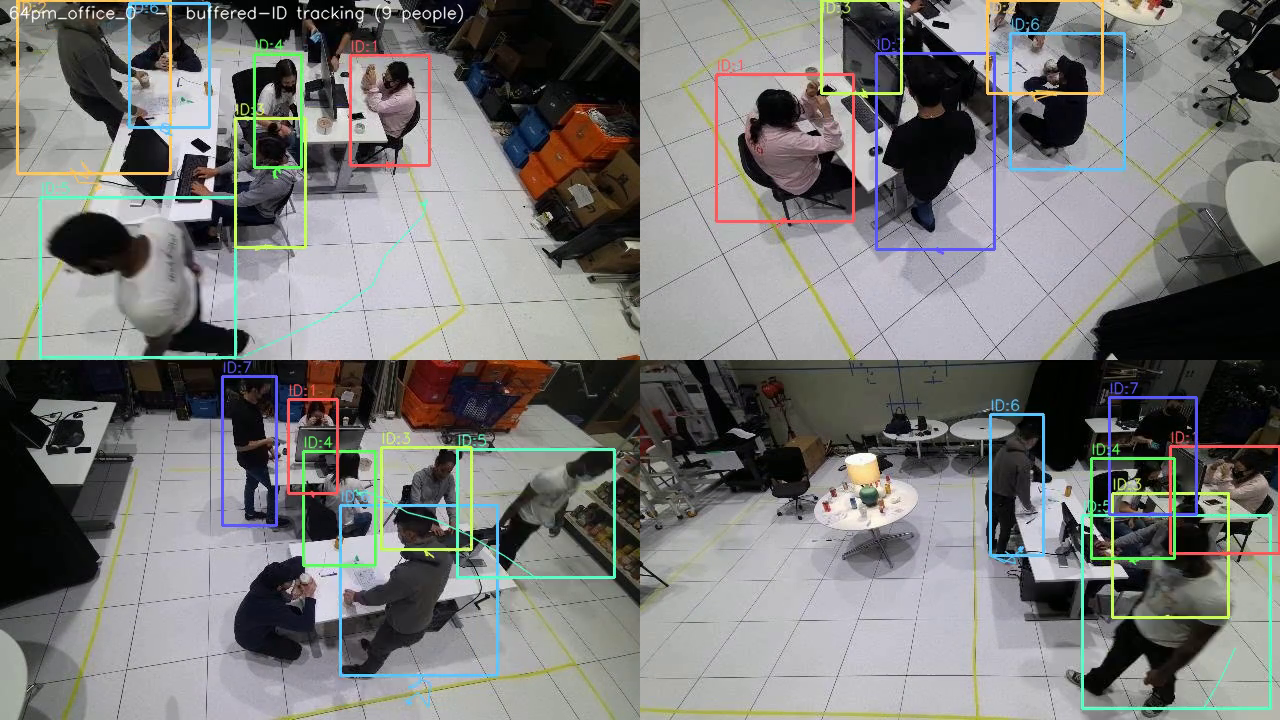
\includegraphics[width=0.92\textwidth]{buffered_camera}
    \caption{Theo dõi đa camera --- office, 4 camera, Buffered ID.}
    \label{fig:multicam_tracking}
\end{figure}

\subsection{Tầng 1: Phát hiện và theo dõi per-camera}

\subsubsection{Phát hiện người}

YOLO11n được fine-tune trên bộ dữ liệu MMPTrack (tập train, session 63am và 64am). Mô hình được xuất sang định dạng ONNX và biên dịch sang TensorRT engine FP16 bằng công cụ của DeepStream. Engine được tự động tạo lần đầu chạy và lưu lại cho các lần sau.

Ngưỡng phát hiện (\texttt{nms-iou}) và ngưỡng tin tưởng được tinh chỉnh theo môi trường. Với môi trường retail, giá trị \texttt{nms-iou = 0,70} giúp tăng recall trong điều kiện che khuất cao.

\subsubsection{Theo dõi cục bộ}

NvDCF chạy ở chế độ Legacy DCF (\texttt{visualTrackerType:1}). Mỗi người được theo dõi độc lập trong từng camera với một local track ID. NvDCF được cấu hình để bật xuất tensor ReID nội tại, mặc dù dự án này sử dụng SGIE bên ngoài thay thế nhằm kiểm soát chất lượng embedding tốt hơn.

\subsubsection{Trích xuất embedding}

Swin-Tiny ReID được triển khai như một mạng SGIE (Secondary GPU Inference Engine) trong DeepStream, xử lý từng bounding box detected. SGIE chạy với tần suất (\texttt{interval}) có thể điều chỉnh --- tức là không nhất thiết phải chạy trên mỗi khung hình --- để giảm tải GPU. Mỗi lần chạy, SGIE cắt ảnh crop từ bounding box, chuẩn hóa về 256$\times$128, và xuất embedding 256 chiều gắn vào metadata của DeepStream.

\subsection{Tầng 2: Định danh xuyên camera}

\subsubsection{CrossCameraGalleryProbe}

\textbf{CrossCameraGalleryProbe} là GStreamer probe tùy chỉnh gắn sau \texttt{nvmultistreamtiler}. Trong mỗi batch, probe thực hiện ba thao tác:

\begin{enumerate}
    \item \textbf{Thu thập:} Đọc embedding và bounding box của tất cả detection từ tất cả camera trong batch.
    \item \textbf{Ghép cặp:} So khớp mỗi tracklet đang hoạt động với gallery Global ID hiện có. Điểm tương đồng kết hợp:
    \begin{equation}\label{eq:score}
        \text{score}(i, j) = (1 - w_g) \cdot \text{cosine}(e_i, e_j) + w_g \cdot \text{geo}(p_i, p_j)
    \end{equation}
    trong đó $e_i, e_j$ là embedding của tracklet $i$ và gallery entry $j$, $\text{geo}(\cdot)$ là điểm tương đồng hình học dựa trên vị trí chân trên mặt phẳng sàn, $w_g$ là trọng số hình học (được chọn là 0{,}25).
    \item \textbf{Gán và cập nhật:} Gán Global ID cho tracklet theo thuật toán Hungarian, cập nhật gallery với embedding mới.
\end{enumerate}

Thuật toán ghép cặp sử dụng ngưỡng \texttt{threshold = 0{,}62} và khoảng cách tối thiểu \texttt{margin = 0{,}02} để tránh ghép cặp mơ hồ.

\subsubsection{Ràng buộc hình học}

Khi có dữ liệu hiệu chỉnh camera (ma trận homography từ MMPTrack), hệ thống chiếu điểm chân (\textit{foot point}) của mỗi bounding box lên mặt phẳng sàn BEV. Khoảng cách Euclid trong không gian sàn được dùng làm ràng buộc bổ sung: hai tracklet từ hai camera chỉ được ghép cặp nếu vị trí trên mặt sàn tương thích.

Ràng buộc hình học chỉ được kích hoạt sau khi có đủ số lượng quan sát tối thiểu (\texttt{geo\_min\_overlaps = 8}) để tránh sai số trong giai đoạn đầu.

\subsubsection{Live ID và Buffered ID}
\label{sec:buffered}

Hệ thống hỗ trợ hai chế độ định danh:

\textbf{Live ID:} Gán Global ID tức thời trong mỗi frame. Ưu điểm: không có độ trễ. Nhược điểm: quyết định sớm có thể bị sai khi người mới vào camera chưa có đủ embedding.

\textbf{Buffered ID (Anchor-Guided):} Tham khảo từ \cite{Huang2023}, chế độ này tích lũy embedding trong cửa sổ trượt 200 khung ($\sim$20 giây, có thể cấu hình qua \texttt{--live-buffered-window}). Sau mỗi cửa sổ, thuật toán anchor-guided clustering xác định các tracklet anchor (embedding ổn định, xuất hiện nhiều camera) và dùng chúng làm trung tâm để gộp các tracklet có liên quan vào cùng Global ID. Chế độ này giới thiệu độ trễ ~20 giây nhưng đạt 97--98\% chất lượng của xử lý offline.

Kết quả Buffered ID được phản hồi lại OSD live theo thời gian thực: module \texttt{live\_buffered} chạy song song, liên tục cập nhật bảng ánh xạ \texttt{(camera, track) $\to$ Global ID}; pipeline đọc bảng này để vẽ Buffered ID ngay trên video live thay cho Live ID. Track mới chưa kịp gom cụm tạm thời hiển thị Live ID rồi tự hội tụ sau một cửa sổ. Nhờ đó video demo không còn hiện tượng phình ID (ví dụ: office chỉ hiển thị 9 ID ổn định thay vì $\sim$98 ID phình do Live ID). Hình~\ref{fig:live_vs_buffered} so sánh trực quan hai chế độ trên cùng 4 camera, và Hình~\ref{fig:bev_tracking} minh họa chế độ BEV với vệt quỹ đạo từng người trên mặt phẳng sàn.

\begin{figure}[H]
    \centering
    \begin{minipage}[t]{0.49\textwidth}
        \centering
        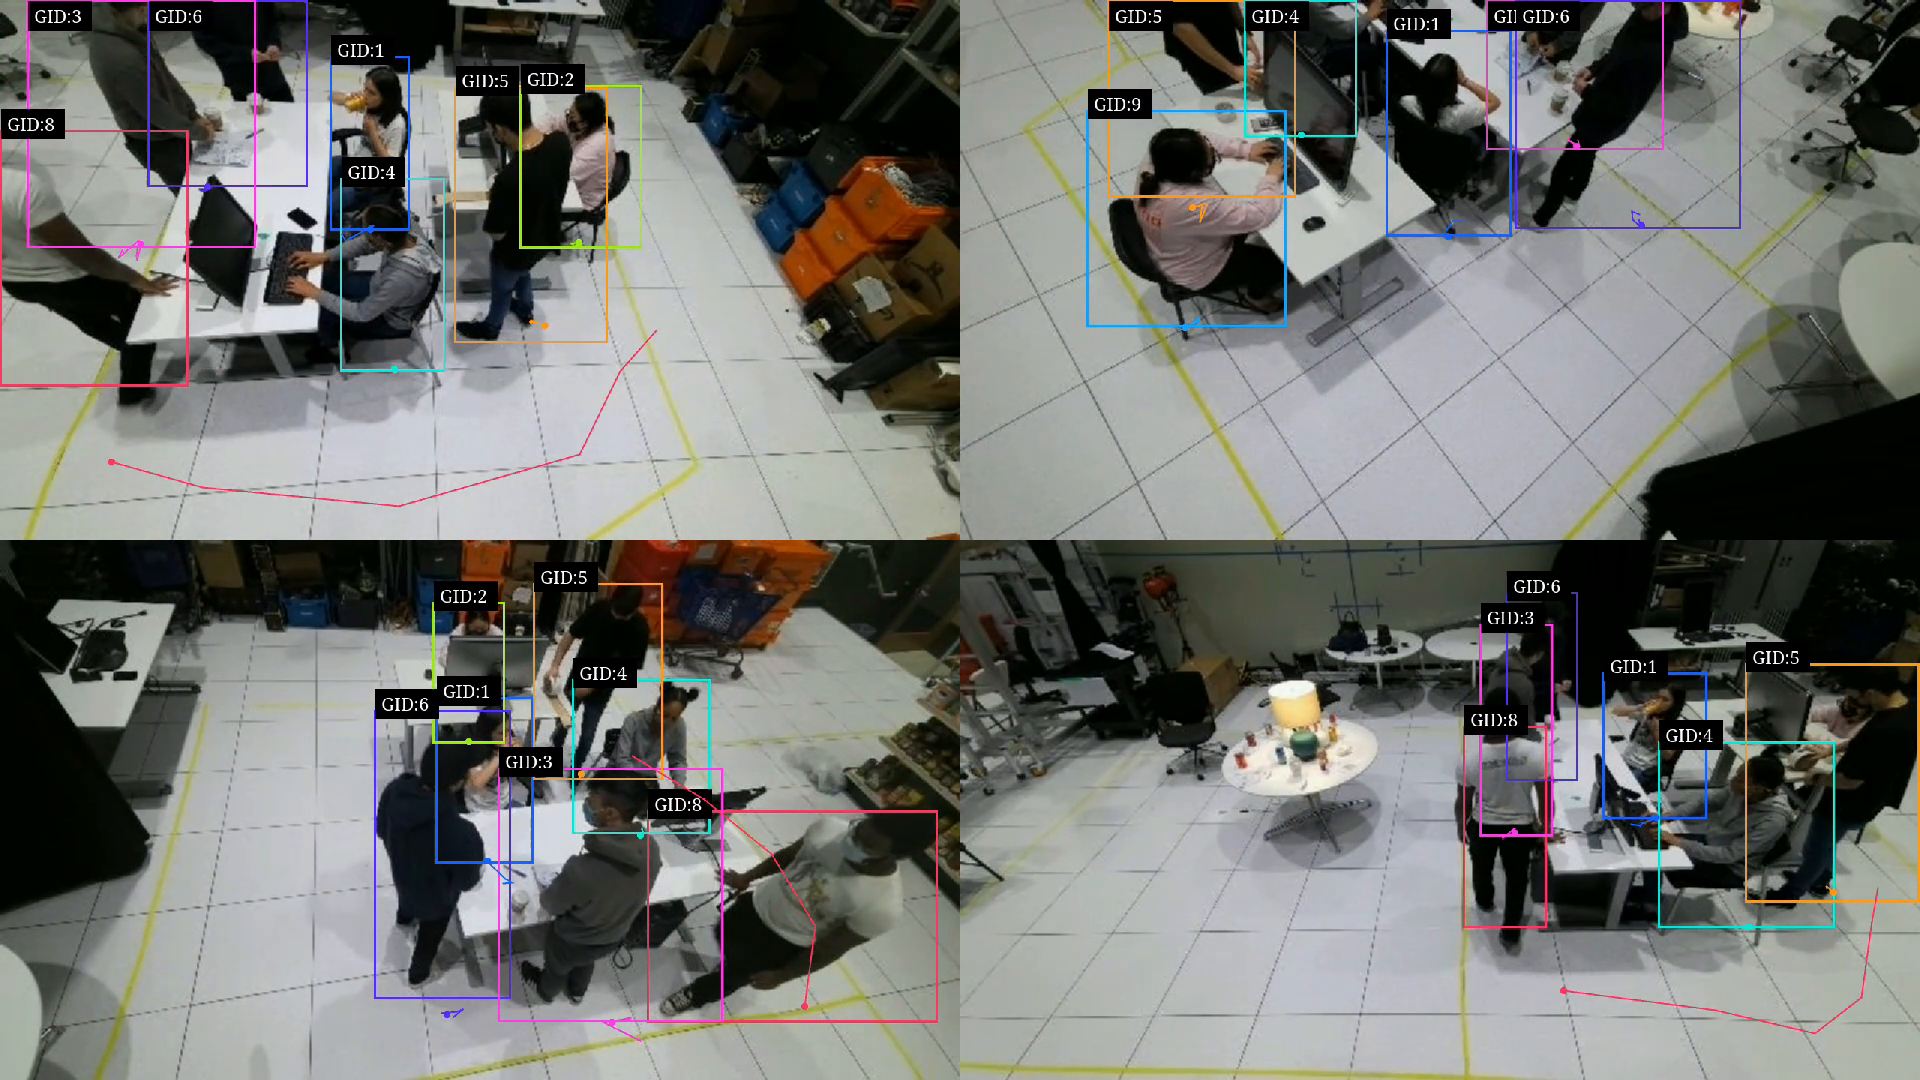
\includegraphics[width=\textwidth]{live_id}
        \small (a) Live ID --- phình định danh (GID:3, GID:6, GID:9\ldots)
    \end{minipage}
    \hfill
    \begin{minipage}[t]{0.49\textwidth}
        \centering
        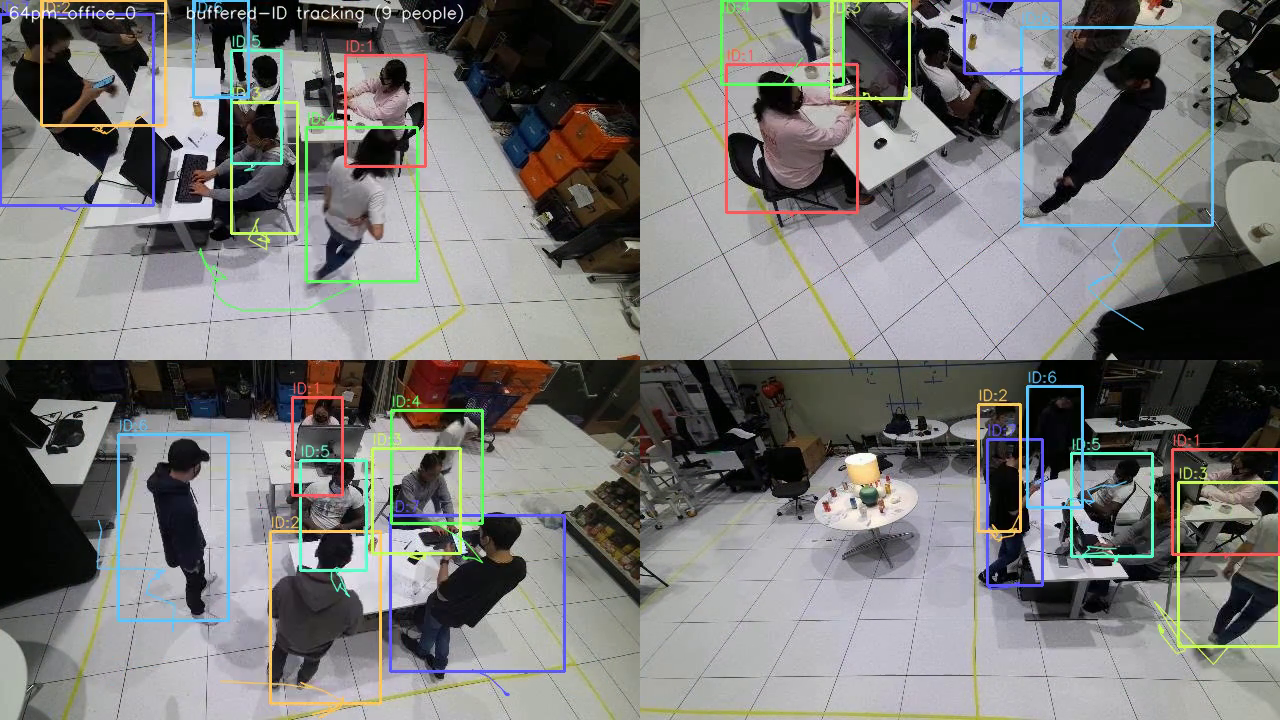
\includegraphics[width=\textwidth]{buffered_camera2}
        \small (b) Buffered ID --- 9 ID ổn định, không còn nhãn `?'
    \end{minipage}
    \caption{So sánh Live ID và Buffered ID --- office, 4 camera.}
    \label{fig:live_vs_buffered}
\end{figure}

\begin{figure}[H]
    \centering
    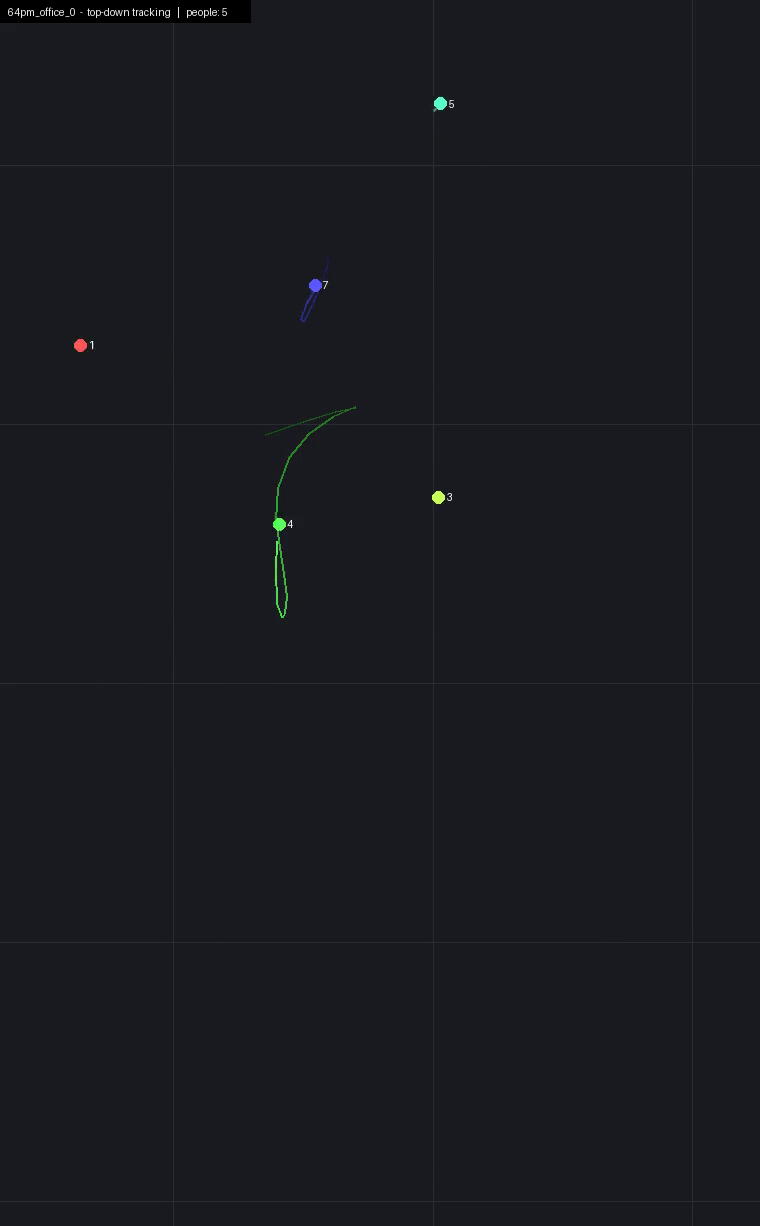
\includegraphics[width=0.65\textwidth]{buffered_bev}
    \caption{Góc nhìn BEV (Bird's-Eye View) --- tracking đa camera, môi trường office.}
    \label{fig:bev_tracking}
\end{figure}

\subsection{Làm sạch nhãn huấn luyện}
\label{sec:label_cleaning}

\subsubsection{Làm sạch nhãn YOLO}

Tập dữ liệu YOLO gốc của MMPTrack được sinh bằng cách \textit{chiếu} hộp 3D của mỗi người vào mọi camera, nên đánh nhãn cả những người bị che khuất hoàn toàn sau kệ hàng/tường  --- những nhãn này nằm trên nền (kệ hàng) và dạy detector ``nền = người'', sinh ra vô số phát hiện lỗi. Đặc biệt là môi trường retail.

Để làm sạch, mô hình YOLO11x độc lập được dùng làm ``bộ xác nhận'' (verifier): mỗi nhãn train chỉ được giữ lại khi bộ xác nhận cũng phát hiện được một người \textit{thực sự nhìn thấy được} chồng lắp với nhãn đó (IoU $>$ ngưỡng). Vì việc làm sạch quá mạnh trên \textit{mọi} môi trường lại loại nhầm cả người bị che khuất một phần nhưng có thật (làm giảm recall ở lobby/office), quy trình cuối cùng \textbf{chỉ áp dụng cho môi trường retail} --- nơi phantom là vấn đề thực --- và giữ nguyên nhãn các môi trường còn lại. Cách làm này loại bỏ $\sim$42\% nhãn retail (chủ yếu là hộp ma trên kệ và hộp bị che khuất hoàn toàn).

Detector được huấn luyện lại trên tập nhãn đã làm sạch. Kết quả: precision phát hiện người trên 20 camera tăng từ 0{,}62 lên 0{,}94, MOTA trung bình per-camera tăng từ 0{,}64 lên 0{,}77, số lần (ID switch) giảm gần một nửa, và Global IDF1 retail tăng 4,5 điểm phần trăm --- trong khi recall ở các môi trường khác được bảo toàn.

\subsubsection{Làm sạch nhãn ReID}

Nhãn \texttt{person\_id} trong MMPTrack được đánh theo từng scene (\textit{scene-local}): cùng một người ở các scene khác nhau có thể có ID khác nhau. Tập train có tới 196 nhãn scene-local khác nhau cho thực tế chỉ 14 người. Điều này làm mô hình ReID nhầm lẫn khi huấn luyện với triplet loss vì cùng một người lại bị coi là nhiều ``lớp'' khác nhau.

Để giải quyết, một công cụ web tương tác (\texttt{reid\_label\_app.py}) được xây dựng để cho phép người dùng gộp các nhãn scene-local về nhãn global. Sau khi gộp thủ công với sự hỗ trợ của công cụ, 196 nhãn scene-local được hợp nhất thành \textbf{56 identity sạch} (14 người nhưng ở 5 môi trường khác nhau). Với nhãn sạch, val gap của mô hình ReID cải thiện từ 0{,}52 lên 0{,}87, và Global IDF1 trên môi trường unseen tăng đáng kể.

\subsection{Phân tích mật độ người (Heatmap)}

\subsubsection{Ba chỉ số phân tích}

Hệ thống bổ sung bộ công cụ phân tích không gian dưới dạng ba loại bản đồ mật độ người. Occupancy, Footfall và Dwell-time là các chỉ số phân tích sử dụng không gian được áp dụng rộng rãi trong giám sát, quản lý cơ sở vật chất và an toàn \cite{Spearpoint2020}; Dwell-time được suy ra từ Occupancy và Footfall theo Định luật Little \cite{Little1961}:

\begin{itemize}
    \item \textbf{Occupancy:} Tổng thời gian người hiện diện trong mỗi ô lưới (tính theo khung hình). Đây là tích lũy đơn giản: mỗi khung hình có người trong ô, cộng 1 vào ô đó.

    \item \textbf{Footfall:} Số người khác nhau (theo Global ID) từng đi qua mỗi ô lưới. Khi một Global ID mới lần đầu xuất hiện trong ô, Footfall của ô tăng lên 1.

    \item \textbf{Dwell-time:} Thời gian dừng trung bình của người trong ô, tính theo công thức Little \cite{Little1961}:
    \begin{equation}
        \text{Dwell-time} = \frac{\text{Occupancy}}{\text{Footfall}}
    \end{equation}
    Công thức này là dạng rời rạc của Định luật Little $W = L/\lambda$ trong lý thuyết hàng đợi.
\end{itemize}

Ba bản đồ tạo thành bộ thông tin bổ sung cho nhau: Occupancy sáng ở nơi người \textit{ở lâu} (bàn làm việc, khu chờ), Footfall sáng ở nơi \textit{nhiều người khác nhau} đi qua (lối đi, cửa), Dwell-time sáng ở nơi \textit{mỗi người dừng lâu} (chỗ ngồi ít người nhưng ở lâu). Hình~\ref{fig:heatmap_cam} minh họa ba bản đồ phủ lên khung hình thực của camera 0 (môi trường office), và Hình~\ref{fig:heatmap_bev} trình bày cùng ba chỉ số trên mặt phẳng sàn BEV gộp tất cả camera.

\begin{figure}[H]
    \centering
    \begin{minipage}[t]{0.32\textwidth}
        \centering
        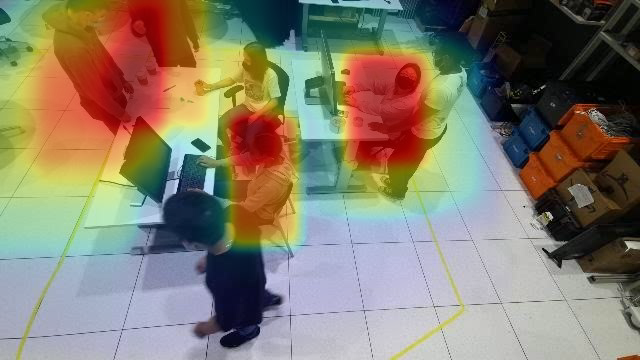
\includegraphics[width=\textwidth]{hm23_cam0_occupancy}
        \small (a) Occupancy
    \end{minipage}
    \hfill
    \begin{minipage}[t]{0.32\textwidth}
        \centering
        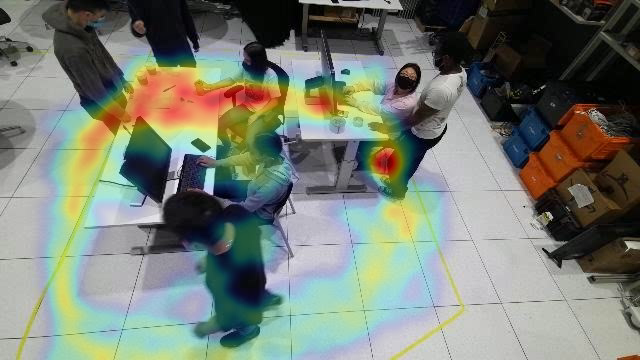
\includegraphics[width=\textwidth]{hm23_cam0_footfall}
        \small (b) Footfall
    \end{minipage}
    \hfill
    \begin{minipage}[t]{0.32\textwidth}
        \centering
        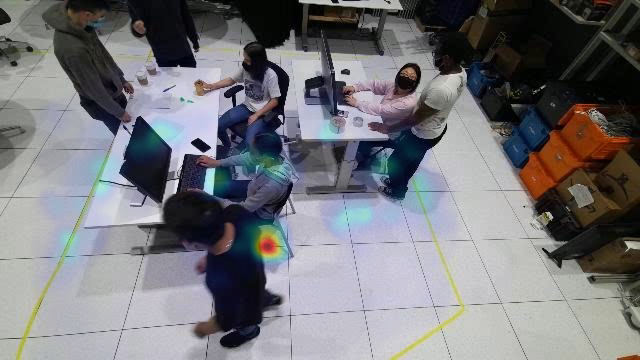
\includegraphics[width=\textwidth]{hm23_cam0_dwelltime}
        \small (c) Dwell-time
    \end{minipage}
    \caption{Heatmap góc camera --- office, cam 0.}
    \label{fig:heatmap_cam}
\end{figure}

\begin{figure}[H]
    \centering
    \begin{minipage}[t]{0.32\textwidth}
        \centering
        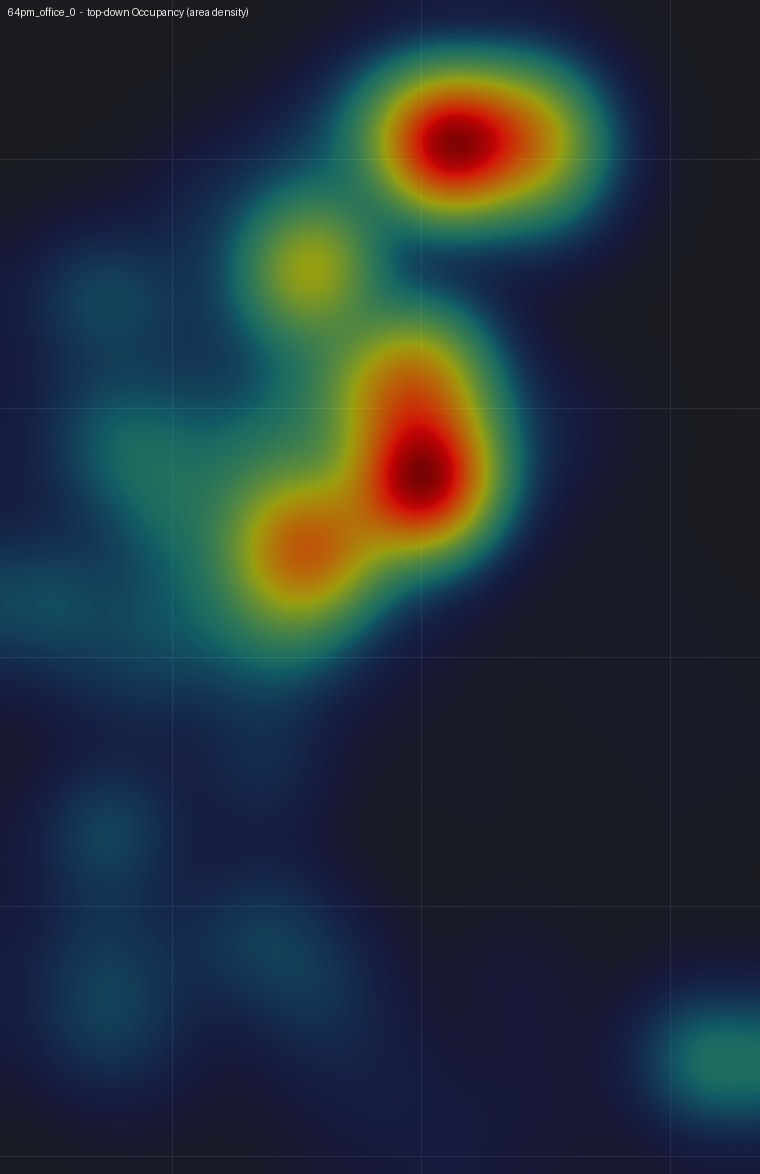
\includegraphics[width=\textwidth]{hm23_bev_occupancy}
        \small (a) Occupancy
    \end{minipage}
    \hfill
    \begin{minipage}[t]{0.32\textwidth}
        \centering
        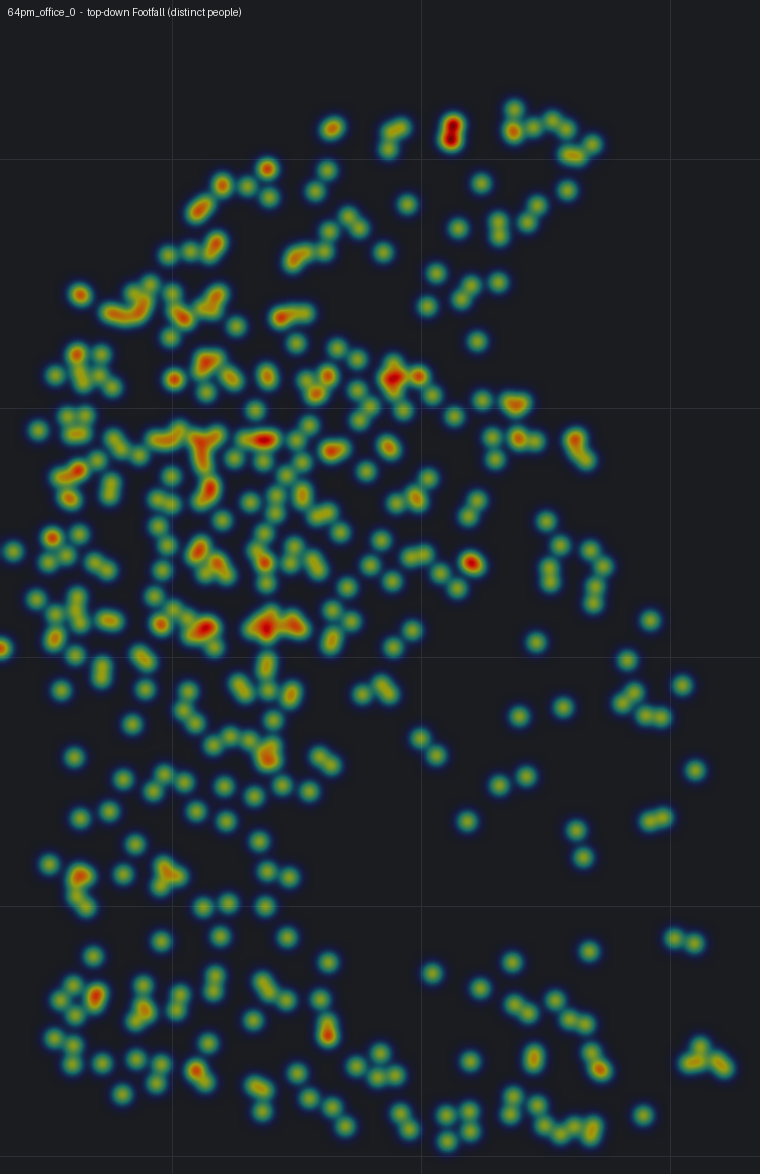
\includegraphics[width=\textwidth]{hm23_bev_footfall}
        \small (b) Footfall
    \end{minipage}
    \hfill
    \begin{minipage}[t]{0.32\textwidth}
        \centering
        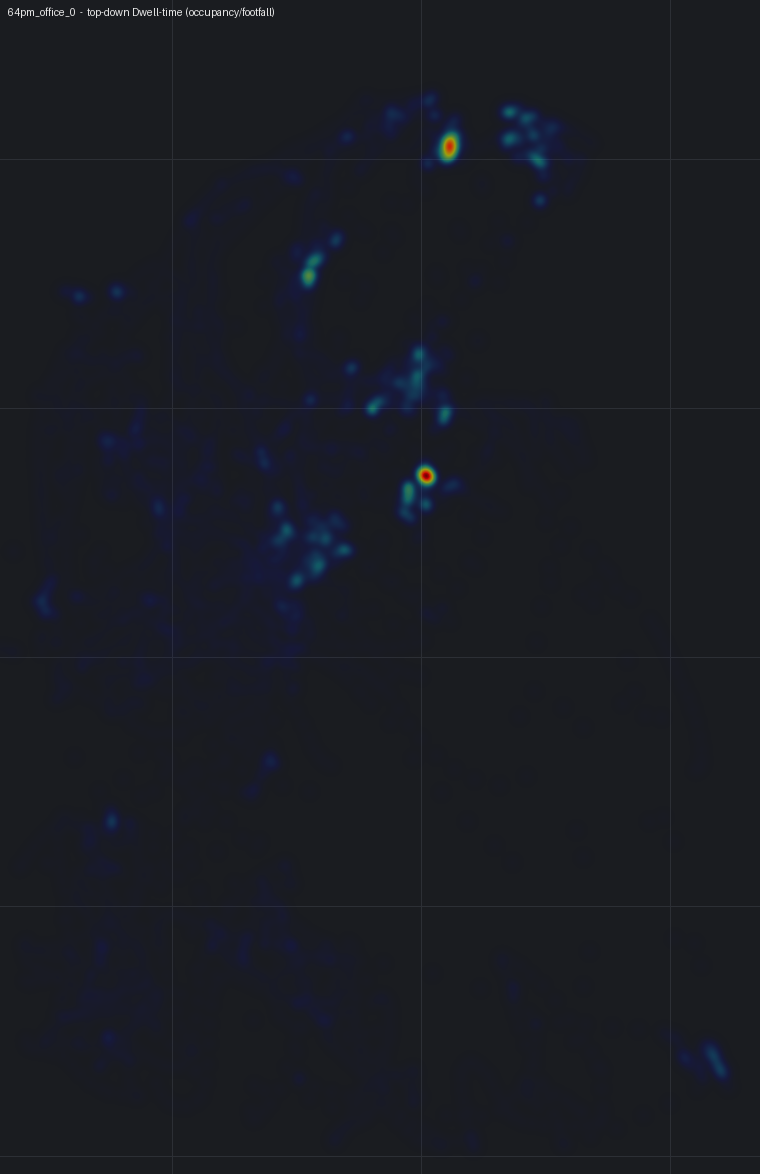
\includegraphics[width=\textwidth]{hm23_bev_dwelltime}
        \small (c) Dwell-time
    \end{minipage}
    \caption{Heatmap BEV mặt sàn --- office, tổng hợp tất cả camera.}
    \label{fig:heatmap_bev}
\end{figure}

\subsubsection{Triển khai thực tế}

Ba chỉ số trên được tính và cập nhật theo thời gian thực trong \textbf{CrossCameraGalleryProbe} (probe tùy chỉnh). Mỗi khung hình, điểm chân của mỗi detection được ánh xạ vào ô lưới tương ứng và cập nhật bộ đếm.

Plugin \texttt{gst-nvdsanalytics} của DeepStream được dùng bổ sung để cung cấp ba chức năng phân tích vùng, chạy trực tiếp trên GPU ngay sau bước tracker:

\begin{enumerate}
    \item \textbf{ROI occupancy --- đếm người trong vùng:} Định nghĩa một vùng sàn (ROI) theo bố cục thực tế của môi trường; plugin đếm số người đang đứng bên trong vùng đó theo thời gian thực. Dùng cho: đo mức sử dụng khu vực.
    \item \textbf{Overcrowding --- cảnh báo quá tải:} Đặt ngưỡng số người cho vùng (chỉnh riêng theo từng môi trường); khi vượt ngưỡng, plugin bật cờ OVERCROWDED. Dùng cho: cảnh báo an toàn.
    \item \textbf{Line-crossing --- đếm băng vạch:} Định nghĩa một vạch ảo có hướng; plugin đếm số người băng qua vạch. Dùng cho: đếm người ra/vào, đo luồng di chuyển (tương ứng metric Footfall).
\end{enumerate}

Mỗi môi trường có một file cấu hình riêng với ROI, vạch đếm và ngưỡng quá tải được chỉnh theo bố cục thực tế (Bảng~\ref{tab:analytics_config}). Hình~\ref{fig:analytics} minh họa các overlay phân tích trên 4 camera: vùng ROI, cảnh báo OVERCROWDED và vạch đếm người ra/vào.

\begin{table}[H]
\centering
\caption[Cấu hình gst-nvdsanalytics theo môi trường]{\bfseries\fontsize{12pt}{0pt}\selectfont Cấu hình phân tích vùng theo môi trường}
\begin{tabular}{|l|l|c|c|}
\hline
\bfseries Môi trường & \bfseries Bố cục & \bfseries Ngưỡng quá tải & \bfseries Số người (Buffered) \\
\hline
Office          & Bàn làm việc             & Mặc định & 9 \\
Café Shop       & Bàn tròn trung tâm, người ngồi & 6 & $\sim$7 \\
Lobby           & Sàn mở, người đi lại     & 6 & 7 \\
Industry Safety & Nhà xưởng, mật độ cao     & 8 & 9 \\
Retail          & Lối đi giữa kệ hàng       & 5 & 10 \\
\hline
\end{tabular}
\label{tab:analytics_config}
\end{table}

\begin{figure}[H]
    \centering
    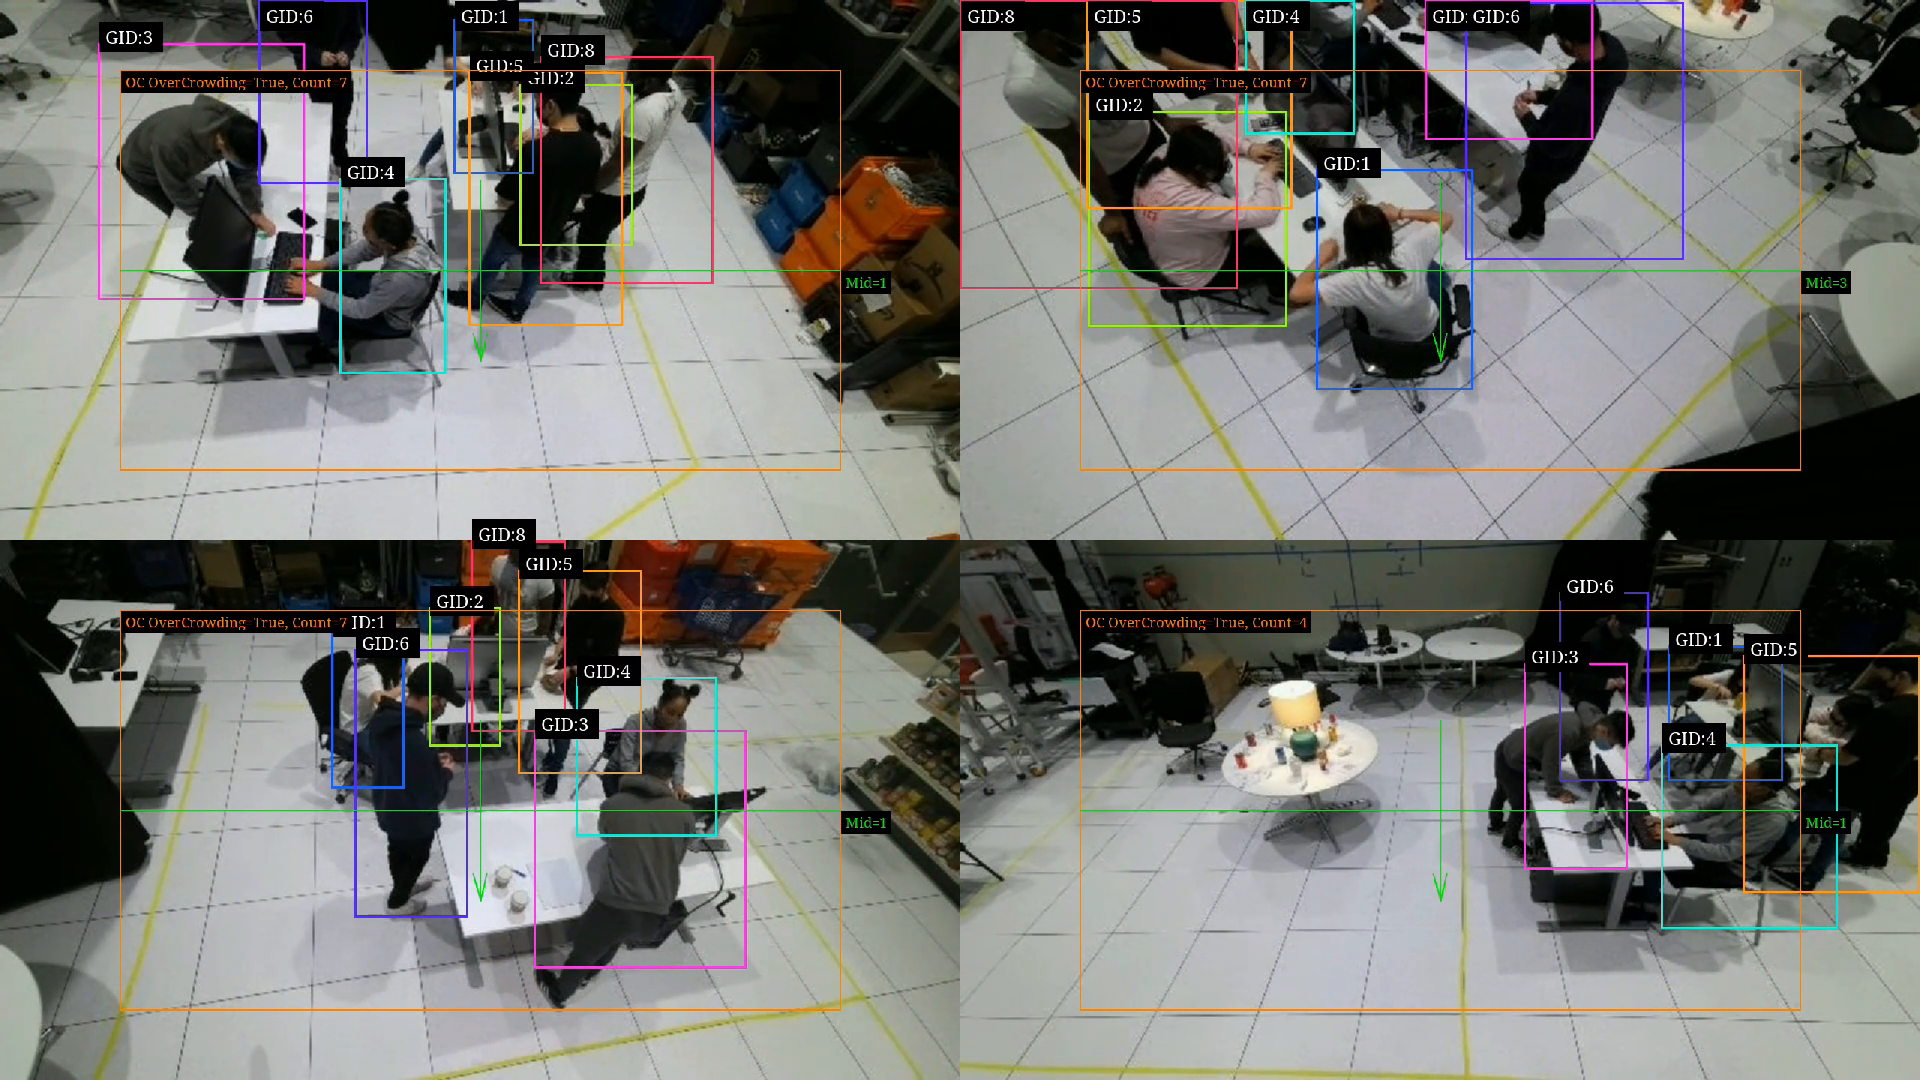
\includegraphics[width=0.92\textwidth]{analytics}
    \caption{Phân tích vùng với \texttt{gst-nvdsanalytics} --- ROI, overcrowding, line-crossing.}
    \label{fig:analytics}
\end{figure}

Ngoài ra, hệ thống cung cấp chế độ \textbf{BEV floor view}: chiếu toàn bộ foot point từ tất cả camera lên bản đồ sàn thực (dùng homography calibration của MMPTrack), cho phép quan sát phân bố người từ góc nhìn từ trên xuống.

\subsection{Triển khai production và giao diện Web}
\label{sec:production_webui}

Ngoài chế độ thí nghiệm (đọc file video để chấm điểm), khi triển khai thực tế hệ thống \textbf{nạp trực tiếp camera RTSP} và phục vụ kết quả cho người vận hành qua một \textbf{giao diện Web (Web UI)}. Hình~\ref{fig:production_arch} mô tả luồng dữ liệu production đầu-cuối.

\begin{figure}[H]
    \centering
    \begin{tikzpicture}[
        font=\small,
        box/.style={draw, rounded corners, align=center, minimum height=1.05cm, fill=LightCyan},
        >={Stealth[length=2.2mm]}, node distance=0.85cm and 1.0cm
    ]
        \node[box, minimum width=2.2cm] (cam) {Camera RTSP\\\texttt{rtsp://}};
        \node[box, right=of cam, minimum width=4.0cm] (ds) {DeepStream\\YOLO11n $\to$ NvDCF\\$\to$ Swin SGIE $\to$ Fusion\\$\to$ OSD Buffered ID};
        \node[box, right=of ds, minimum width=2.0cm] (hls) {HLS\\\texttt{hlssink2}};
        \node[box, below=of ds, minimum width=4.0cm] (meta) {Metadata (CSV/NPZ)\\$\to$ SQLite};
        \node[box, right=of meta, minimum width=2.0cm] (rag) {RAG backend\\FastAPI + tool-use};
        \node[box, right=of hls, minimum width=3.0cm] (web) {Web UI (trình duyệt)\\Live $\cdot$ Dashboard\\ROI $\cdot$ Heatmap $\cdot$ Ask};
        \draw[->] (cam) -- (ds);
        \draw[->] (ds) -- (hls);
        \draw[->] (hls) -- (web);
        \draw[->] (ds) -- (meta);
        \draw[->] (meta) -- (rag);
        \draw[->] (rag) -| (web);
    \end{tikzpicture}
    \caption{Kiến trúc triển khai production}
    \label{fig:production_arch}
\end{figure}

Toàn bộ chuỗi \texttt{RTSP $\to$ DeepStream (OSD Buffered ID) $\to$ HLS $\to$ trình duyệt} chạy thời gian thực ở $\sim$15 FPS/camera (RTP-over-TCP, \texttt{hlssink2 sync=0}). Pipeline đồng thời ghi metadata theo dõi (định danh, quỹ đạo, vùng) vào CSDL SQLite; một backend FastAPI phục vụ các view của Web UI:

\begin{itemize}
    \item \textbf{Live Wall} --- xem trực tiếp OSD nhiều camera qua HLS;
    \item \textbf{Dashboard} --- KPI hệ thống (IDF1, FPS, VRAM) và dòng cảnh báo;
    \item \textbf{ROI editor} --- vẽ vùng/vạch trực tiếp trên khung hình và tạo cấu hình nvdsanalytics đúng định dạng;
    \item \textbf{Heatmap} --- Occupancy/Footfall/Dwell-time theo camera và BEV;
    \item \textbf{Ask} --- hỏi-đáp ngôn ngữ tự nhiên trên metadata theo dõi (tác tử gọi-công-cụ): tìm người theo ảnh, dwell theo vùng, quỹ đạo BEV, vùng đông nhất.
\end{itemize}

Hình~\ref{fig:webui} minh hoạ một số view của Web UI.

\begin{figure}[H]
    \centering
    \begin{minipage}[t]{0.48\textwidth}
        \centering
        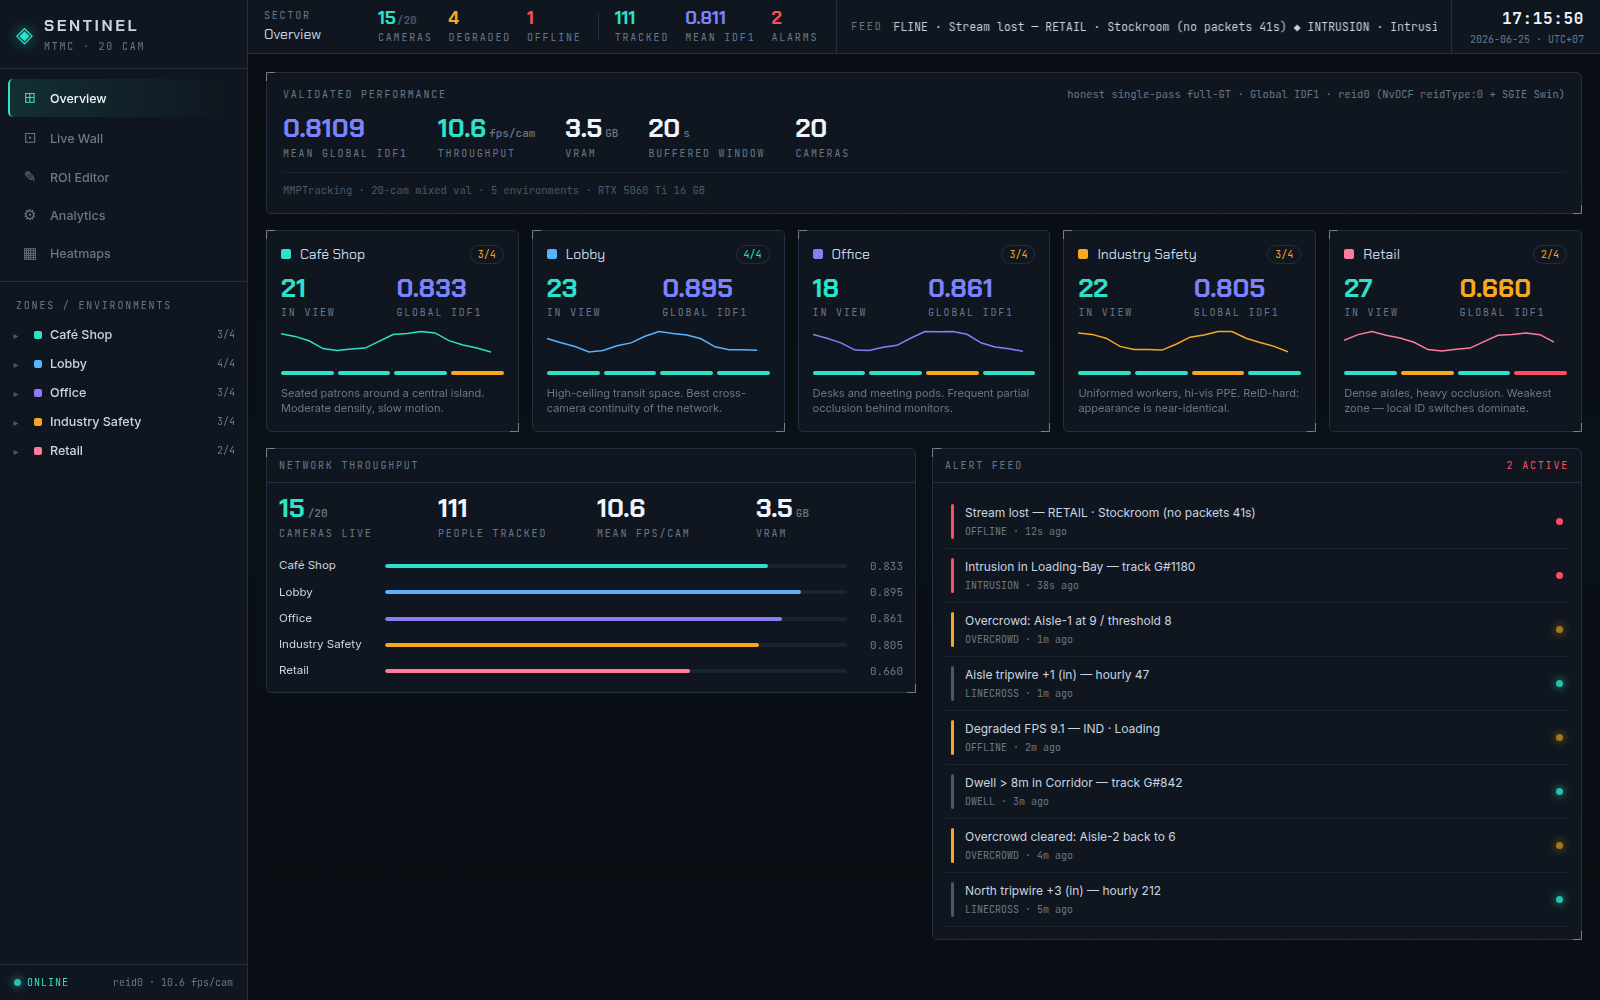
\includegraphics[width=\textwidth]{webui_dashboard}
        \small (a) Dashboard
    \end{minipage}
    \hfill
    \begin{minipage}[t]{0.48\textwidth}
        \centering
        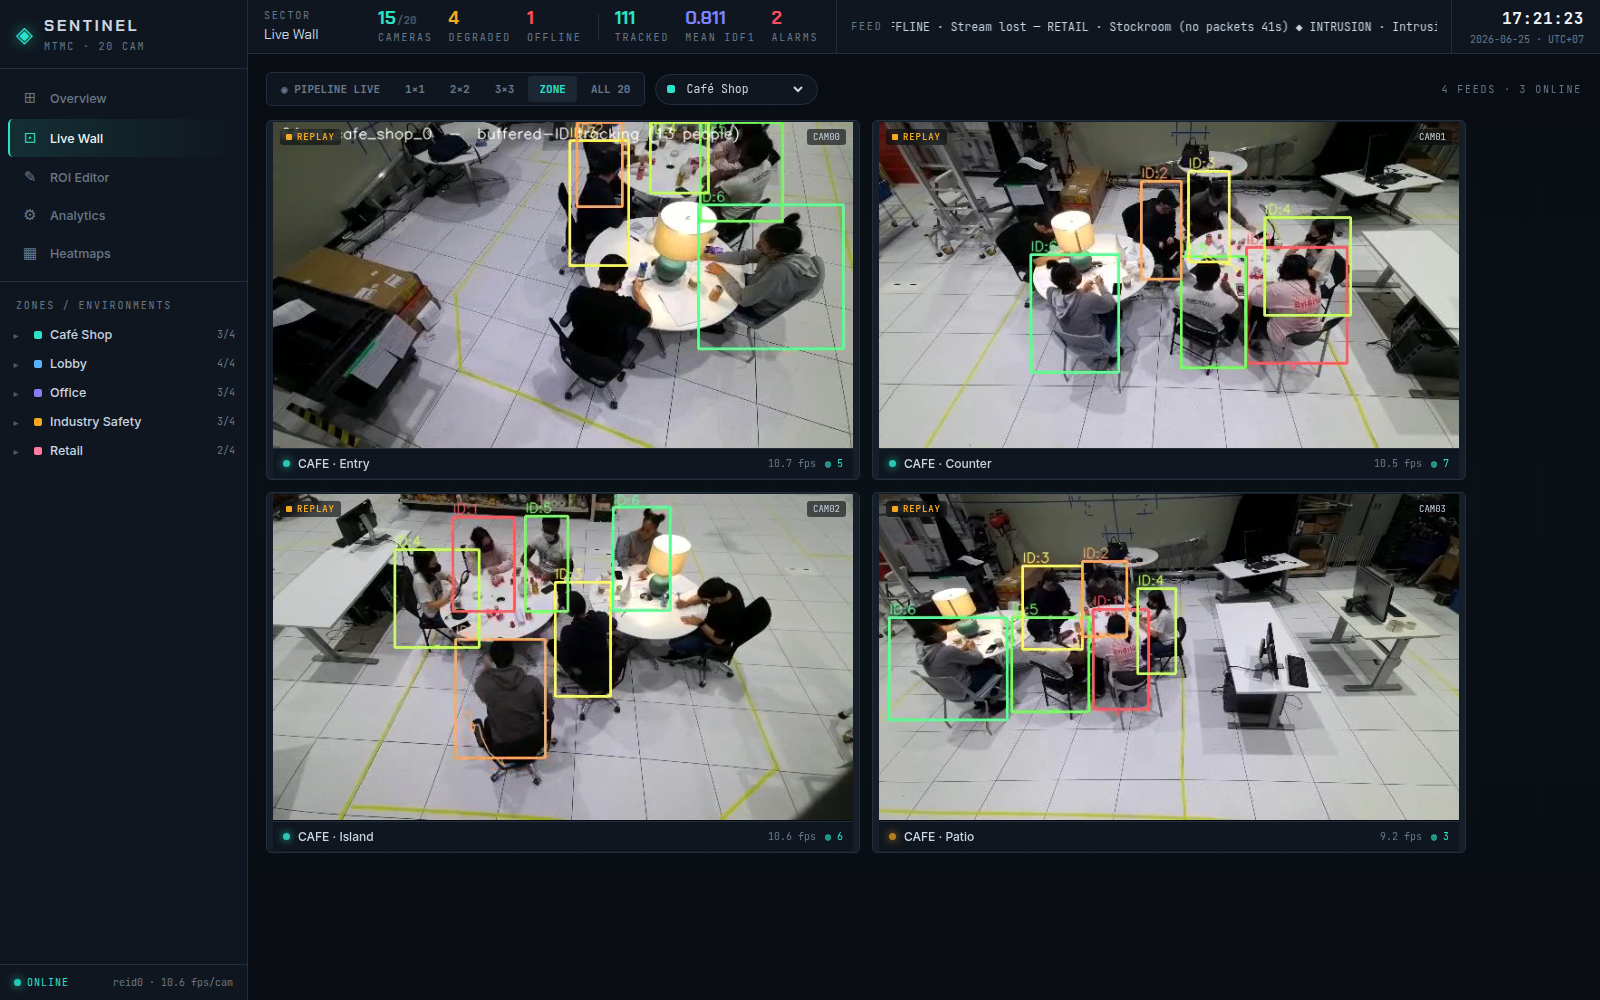
\includegraphics[width=\textwidth]{webui_live_cafe}
        \small (b) Live Wall
    \end{minipage}
    \\[6pt]
    \begin{minipage}[t]{0.48\textwidth}
        \centering
        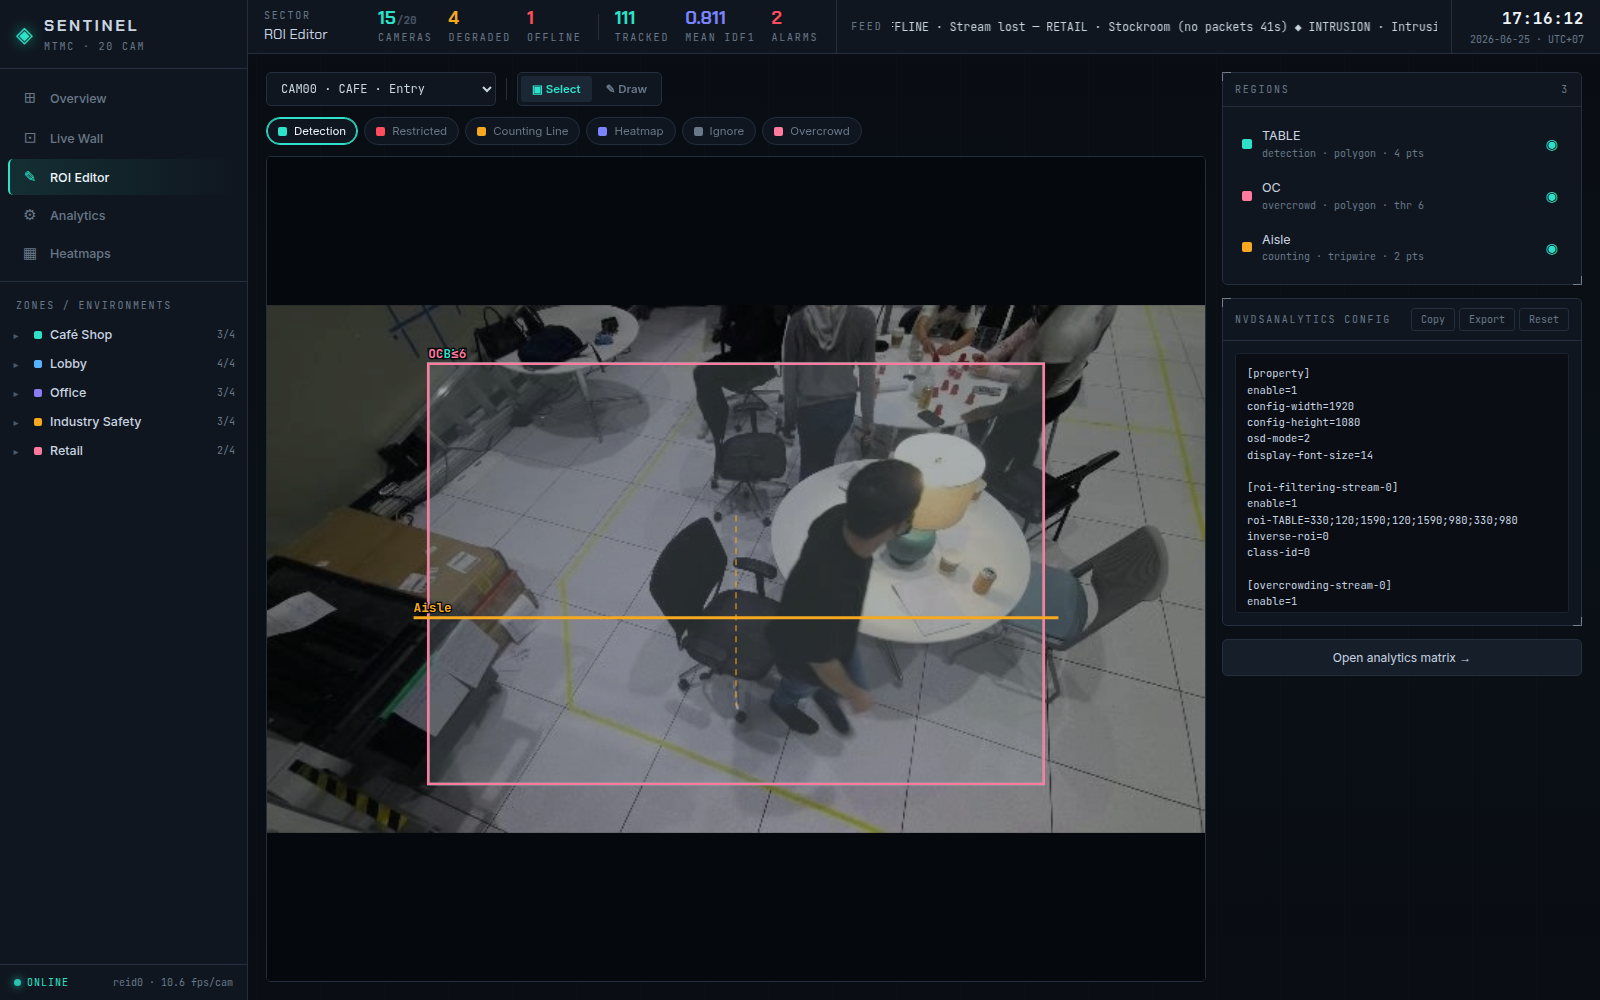
\includegraphics[width=\textwidth]{webui_roi_editor}
        \small (c) ROI editor
    \end{minipage}
    \hfill
    \begin{minipage}[t]{0.48\textwidth}
        \centering
        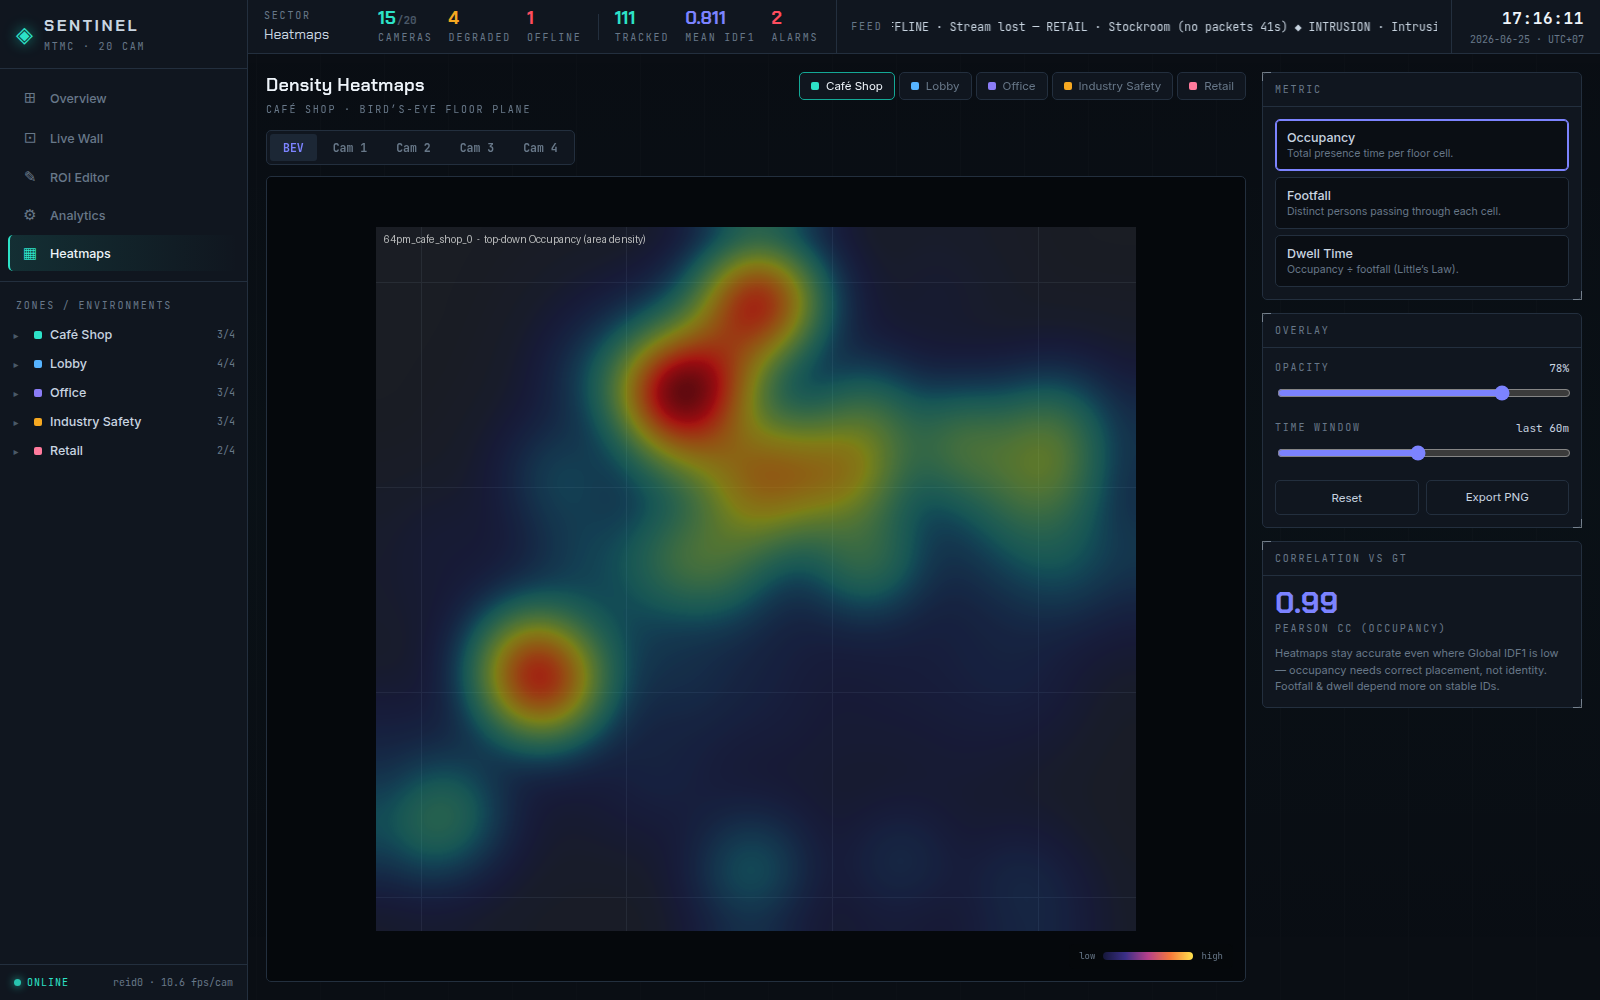
\includegraphics[width=\textwidth]{webui_heatmap}
        \small (d) Heatmap
    \end{minipage}
    \caption{Giao diện Web của hệ thống --- Dashboard, Live Wall, ROI editor và Heatmap.}
    \label{fig:webui}
\end{figure}

\newpage

%%%%%%%%%%%%%%%%%%%%%%%%%%%%%%%%%%%%%%%%%%%%%%%%%%
%               CHƯƠNG 4: THỰC NGHIỆM VÀ KẾT QUẢ
%%%%%%%%%%%%%%%%%%%%%%%%%%%%%%%%%%%%%%%%%%%%%%%%%%
\section*{CHƯƠNG 4.  THỰC NGHIỆM VÀ KẾT QUẢ}
\addcontentsline{toc}{section}{\numberline{}CHƯƠNG 4.  THỰC NGHIỆM VÀ KẾT QUẢ}
\setcounter{section}{4}
\setcounter{subsection}{0}
\setcounter{figure}{0}
\setcounter{table}{0}

\subsection{Cấu hình thực nghiệm}

\subsubsection{Phần cứng và phần mềm}

Tất cả thực nghiệm được thực hiện trên cấu hình:

\begin{table}[H]
    \centering
    \caption[Cấu hình phần cứng thực nghiệm]{\bfseries\fontsize{12pt}{0pt}\selectfont Cấu hình phần cứng thực nghiệm}
    \begin{tabular}{|l|l|}
    \hline
    \bfseries Thành phần & \bfseries Thông số \\
    \hline
    GPU & NVIDIA RTX 5060 Ti (16 GB VRAM) \\
    Hệ điều hành & Ubuntu 24.04 \\
    DeepStream & NVIDIA DeepStream SDK 9.0 \\
    Python & 3.12 \\
    TensorRT & 10.14 \\
    CUDA & 13.1 \\
    \hline
    \end{tabular}
    \label{tab:hardware}
\end{table}

\subsubsection{Bộ dữ liệu kiểm thử}

Kiểm thử được thực hiện trên tập validation \textit{session 64pm} của MMPTrack gồm 24 scene thuộc 5 môi trường. Mỗi scene bao gồm 3--5 camera. Tất cả người trong tập validation là \textit{unseen subjects} --- không xuất hiện trong tập train.

\subsubsection{Cấu hình pipeline}

Pipeline được chạy với preset mặc định: NvDCF Legacy DCF với ReID nội tại tắt, Swin-Tiny SGIE là nguồn embedding duy nhất. Các thông số ReID chính: \texttt{threshold = 0{,}62}, \texttt{margin = 0{,}02}, \texttt{geo\_weight = 0{,}25}, \texttt{geo\_min\_overlaps = 8}.

\subsection{Kết quả định danh xuyên camera}

\subsubsection{Global IDF1 theo môi trường}

Bảng~\ref{tab:results} trình bày kết quả Global IDF1 của hệ thống trên toàn bộ tập validation MMPTrack --- 24 scene thuộc 5 môi trường --- so sánh với phương pháp baseline DMCT-Ext-TD \cite{Han2022}.

\begin{table}[H]
    \centering
    \caption[Kết quả Global IDF1 theo môi trường --- toàn tập validation]{\bfseries\fontsize{12pt}{0pt}\selectfont Kết quả Global IDF1 theo môi trường (toàn tập validation: 24 scene)}
    \begin{tabular}{|l|c|c|c|}
    \hline
    \bfseries Môi trường & \bfseries Số scene & \bfseries Toàn tập val & \bfseries Baseline \cite{Han2022} \\
    \hline
    Lobby    & 4 & 0,906 & --- \\
    Office   & 3 & 0,880 & --- \\
    Industry & 5 & 0,847 & --- \\
    Café     & 4 & 0,839 & --- \\
    Retail   & 8 & 0,661 & --- \\
    \hline
    \bfseries Trung bình & \bfseries 24 & \bfseries 0,798 & \bfseries 0,741 \\
    \hline
    \end{tabular}
    \label{tab:results}
\end{table}

Trên toàn tập 24 cảnh, hệ thống đạt Global IDF1 trung bình \textbf{0,798} --- vượt baseline \cite{Han2022} 5,7 điểm phần trăm. Bốn trong năm môi trường (lobby, office, industry, café) đều vượt ngưỡng mục tiêu 0,8. Retail là môi trường duy nhất không đạt ngưỡng này, với IDF1 trung bình 0,661 trên 8 cảnh.

Kết quả này đạt được sau khi huấn luyện lại detector YOLO11n trên tập nhãn retail đã làm sạch (Phần~\ref{sec:label_cleaning}): so với detector cũ (huấn luyện trên nhãn gốc còn nhiễu phantom), Global IDF1 toàn tập tăng từ 0,774 lên 0,798, riêng retail tăng 4,5 điểm phần trăm (0,616 $\to$ 0,661) và \textit{precision} phát hiện người tăng vọt từ 0,62 lên 0,94 --- xác nhận các bounding box ``ma'' trên kệ hàng đã được loại bỏ tận gốc. Các môi trường không-retail cũng không bị ảnh hưởng (thậm chí nhỉnh hơn nhẹ) vì nhãn của chúng được giữ nguyên.

Mức chênh giữa các cảnh trong cùng môi trường là đáng kể: ví dụ retail\_3 (0,721) dễ hơn nhiều so với retail\_1 (0,597, cảnh khó nhất toàn tập).

\subsubsection{Phân tích theo môi trường}

Lobby (0,906) và office (0,880) đạt cao nhất nhờ điều kiện thuận lợi: lối đi rõ ràng, ánh sáng tốt, ít chồng lấn giúp ReID phân biệt dễ dàng. Industry (0,847) vẫn đạt ngưỡng mục tiêu dù người mặc đồng phục lao động --- Buffered ID với cửa sổ 20 giây tích lũy đủ bằng chứng để gán đúng định danh. Café (0,839) cho kết quả tốt nhưng biến thiên đáng kể giữa các cảnh (0,733--0,931). Retail (0,661) là môi trường yếu nhất: dù huấn luyện lại detector trên nhãn sạch đã nâng kết quả từ 0,616, kệ hàng cao vẫn che khuất khiến detector bỏ sót nhiều người thực (recall giảm) --- giới hạn vật lý không khắc phục được bằng thuật toán, cũng phản ánh qua việc $\sim$42\% nhãn YOLO gốc của retail là phantom hoặc bị che khuất.

Hình~\ref{fig:pipeline_all_osd} trình bày đầu ra pipeline trên cả 5 môi trường --- mỗi ô là khung hình tổng hợp 4 camera với bounding box màu riêng và nhãn Buffered ID. Hình~\ref{fig:pipeline_all_bev} hiển thị cùng 5 môi trường ở góc nhìn BEV, cho thấy vệt quỹ đạo di chuyển của từng người trên mặt phẳng sàn.

\begin{figure}[H]
    \centering
    \begin{minipage}[t]{0.48\textwidth}
        \centering
        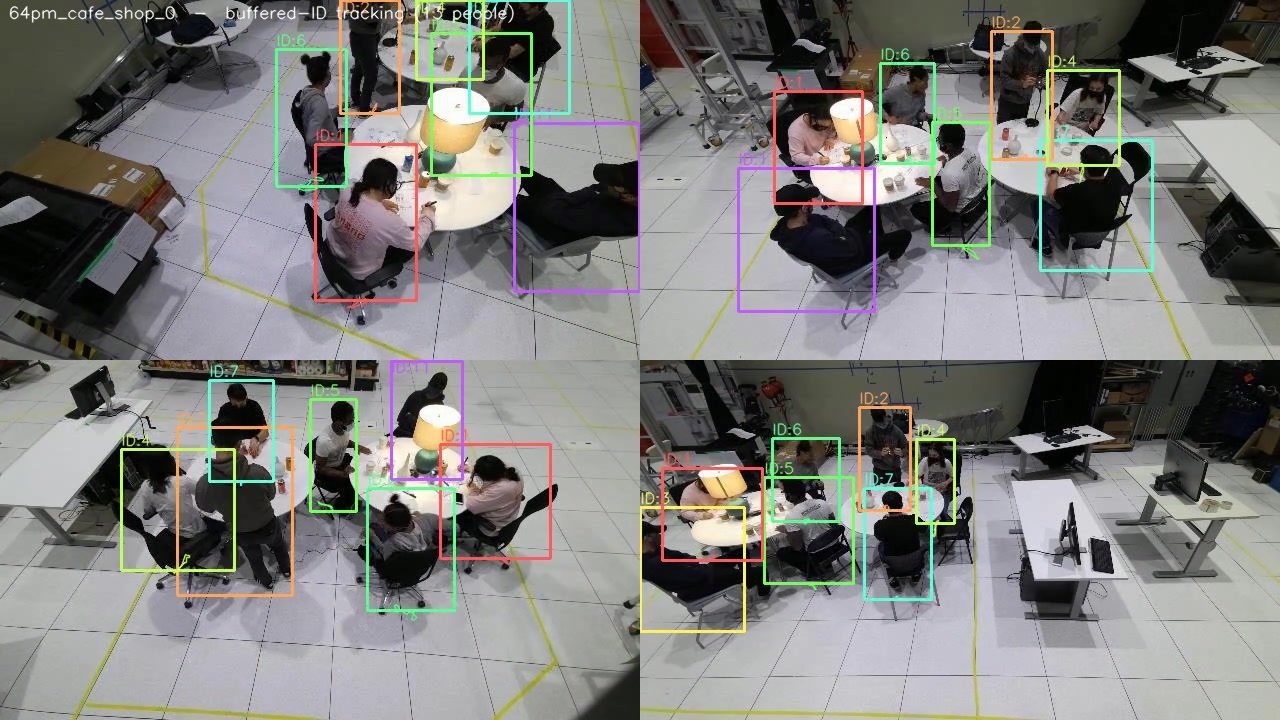
\includegraphics[width=\textwidth]{pipeline_cafe_shop_osd}
        \small (a) Café
    \end{minipage}
    \hfill
    \begin{minipage}[t]{0.48\textwidth}
        \centering
        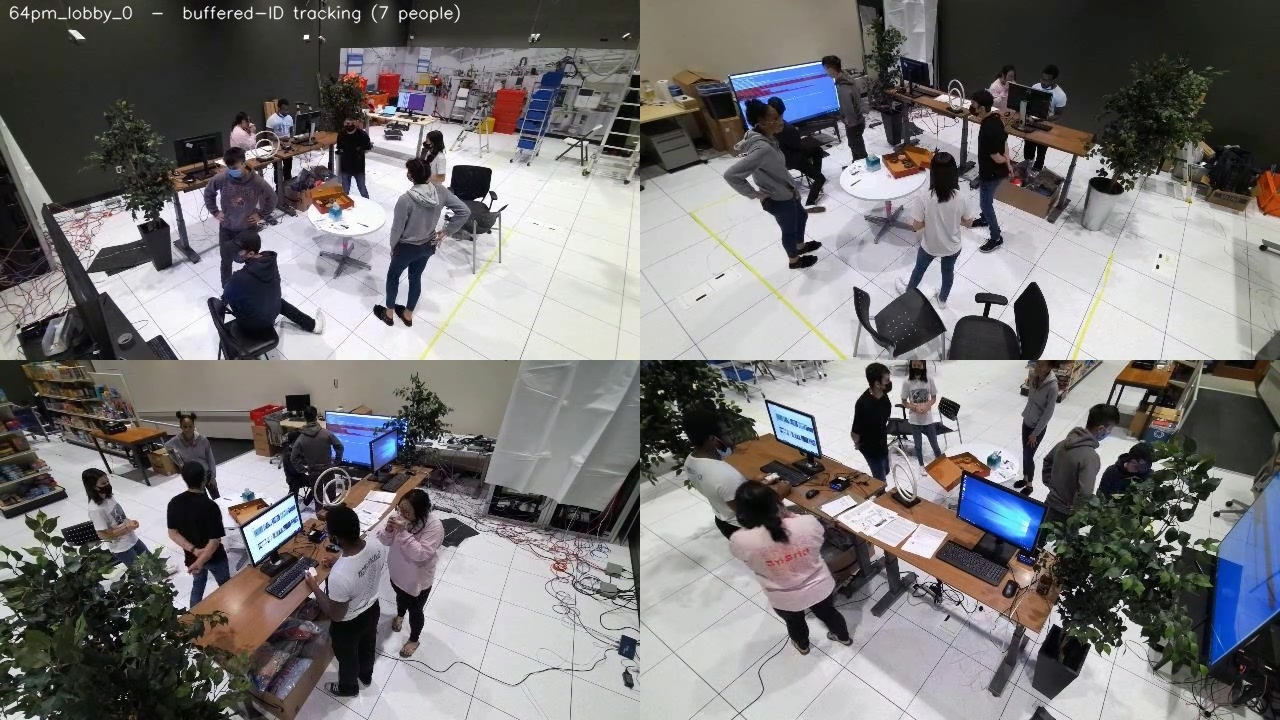
\includegraphics[width=\textwidth]{pipeline_lobby_osd}
        \small (b) Lobby
    \end{minipage}
    \\[6pt]
    \begin{minipage}[t]{0.48\textwidth}
        \centering
        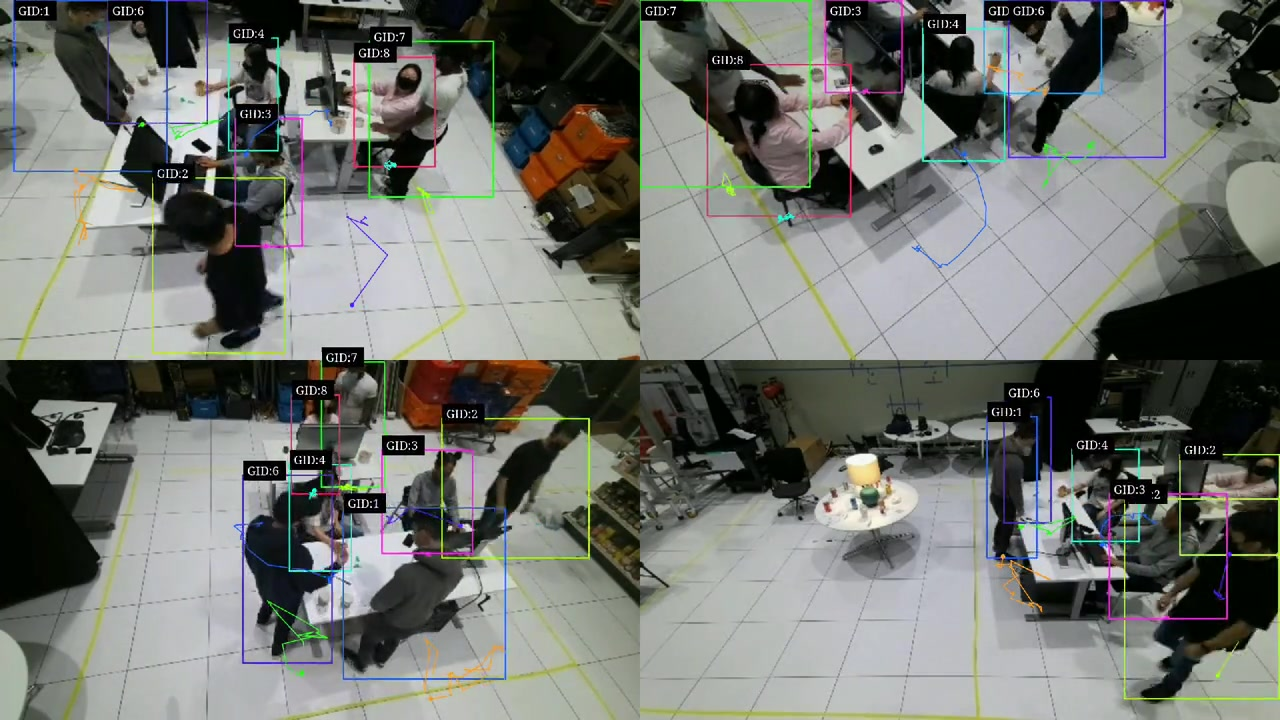
\includegraphics[width=\textwidth]{pipeline_office_osd}
        \small (c) Office
    \end{minipage}
    \hfill
    \begin{minipage}[t]{0.48\textwidth}
        \centering
        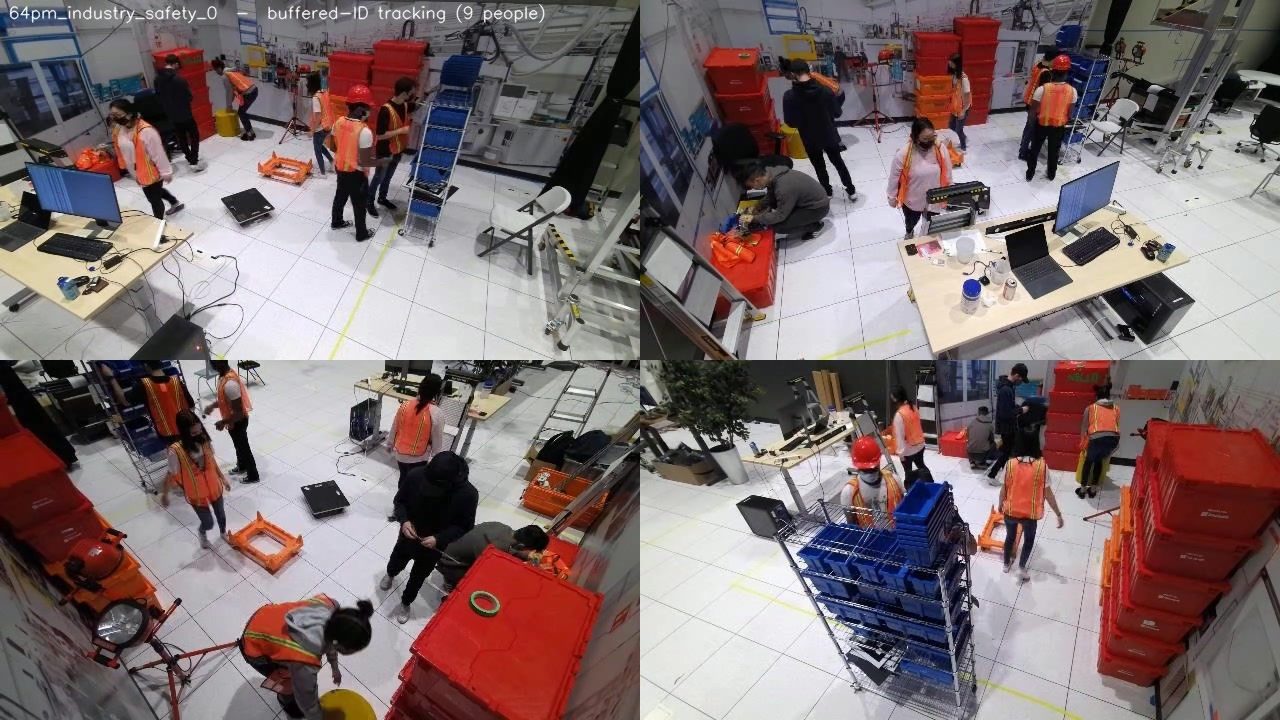
\includegraphics[width=\textwidth]{pipeline_industry_safety_osd}
        \small (d) Industry
    \end{minipage}
    \\[6pt]
    \begin{minipage}[t]{0.60\textwidth}
        \centering
        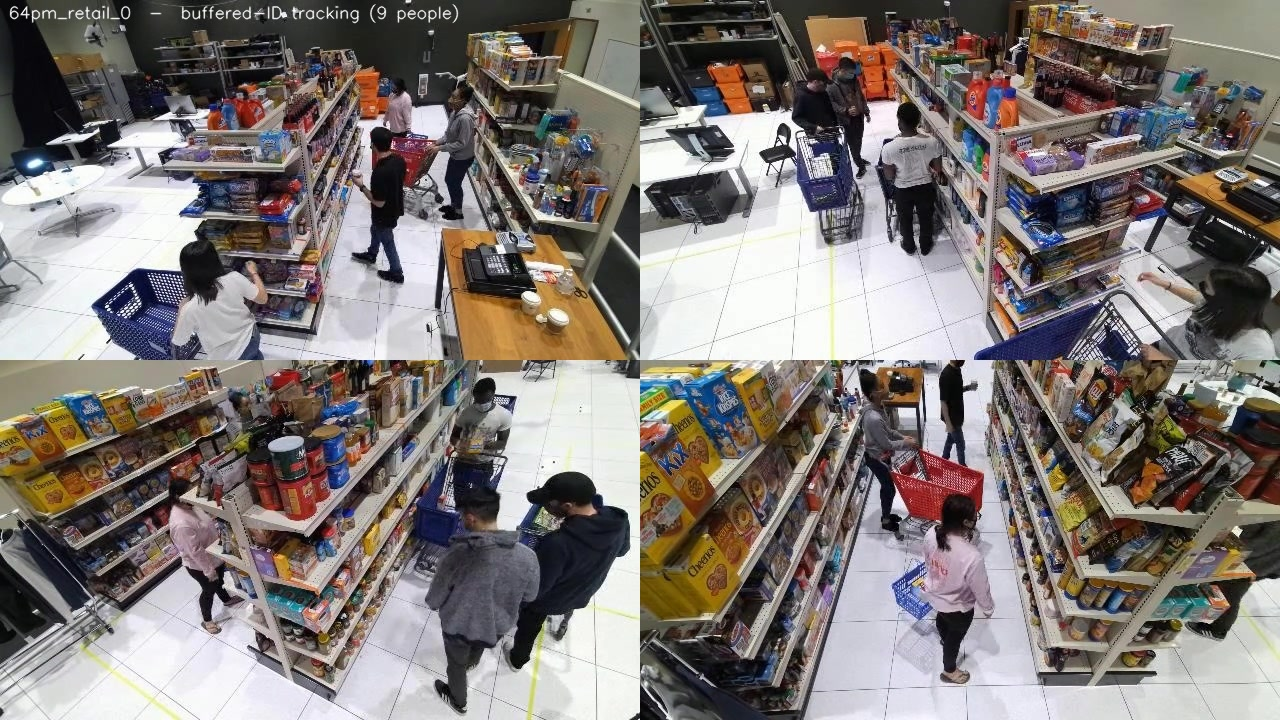
\includegraphics[width=\textwidth]{pipeline_retail_osd}
        \small (e) Retail
    \end{minipage}
    \caption{Kết quả theo dõi Buffered ID trên 5 môi trường --- bounding box màu riêng, nhãn Global ID nhất quán xuyên camera.}
    \label{fig:pipeline_all_osd}
\end{figure}

\begin{figure}[H]
    \centering
    \begin{minipage}[t]{0.32\textwidth}
        \centering
        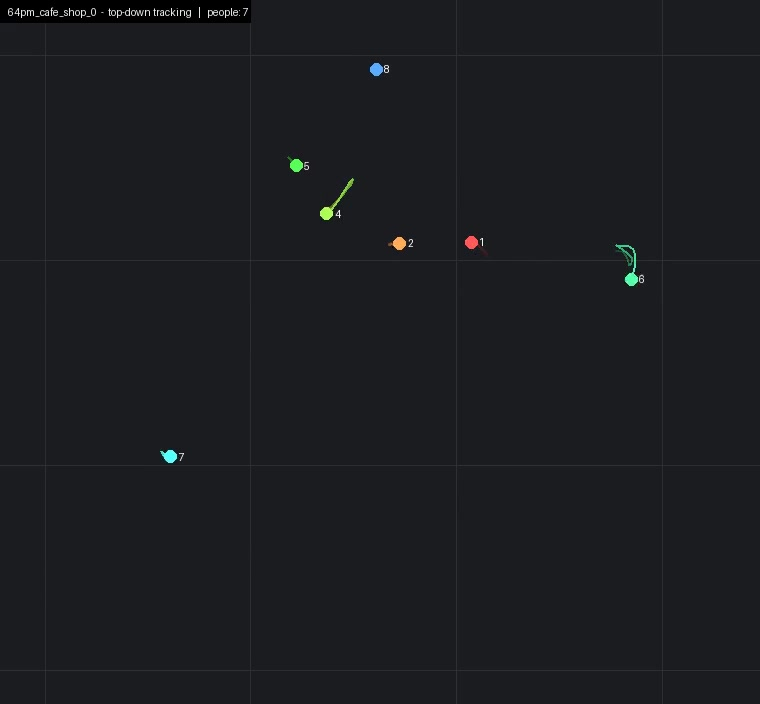
\includegraphics[width=\textwidth]{pipeline_cafe_shop_bev}
        \small (a) Café
    \end{minipage}
    \hfill
    \begin{minipage}[t]{0.32\textwidth}
        \centering
        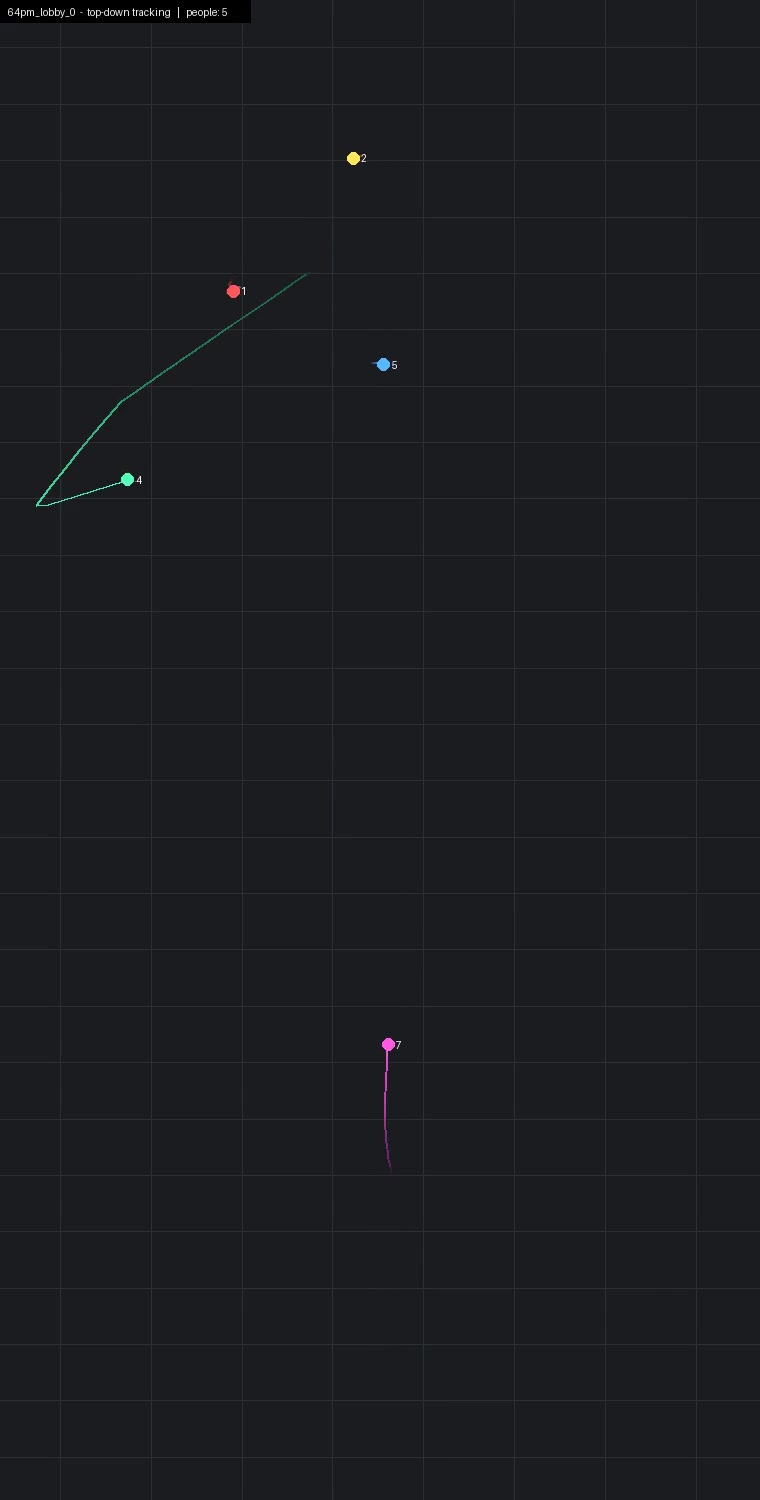
\includegraphics[width=\textwidth]{pipeline_lobby_bev}
        \small (b) Lobby
    \end{minipage}
    \hfill
    \begin{minipage}[t]{0.32\textwidth}
        \centering
        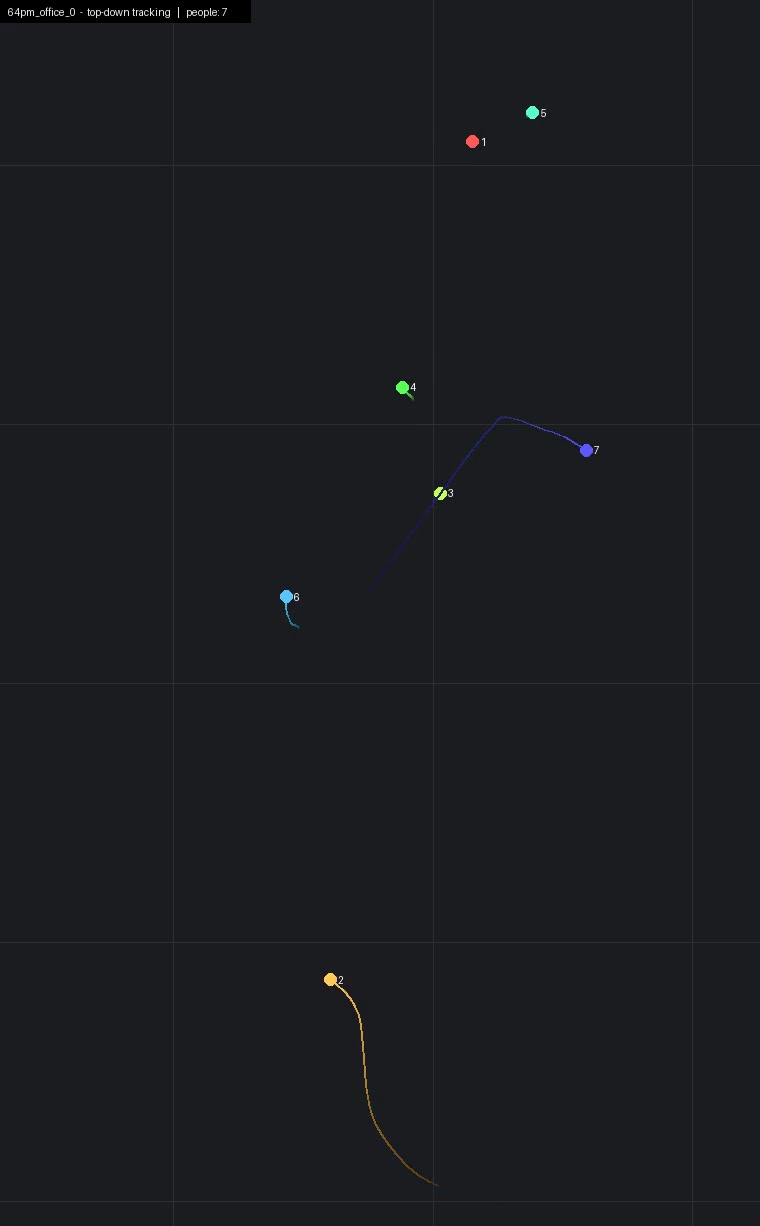
\includegraphics[width=\textwidth]{pipeline_office_bev}
        \small (c) Office
    \end{minipage}
    \\[6pt]
    \begin{minipage}[t]{0.48\textwidth}
        \centering
        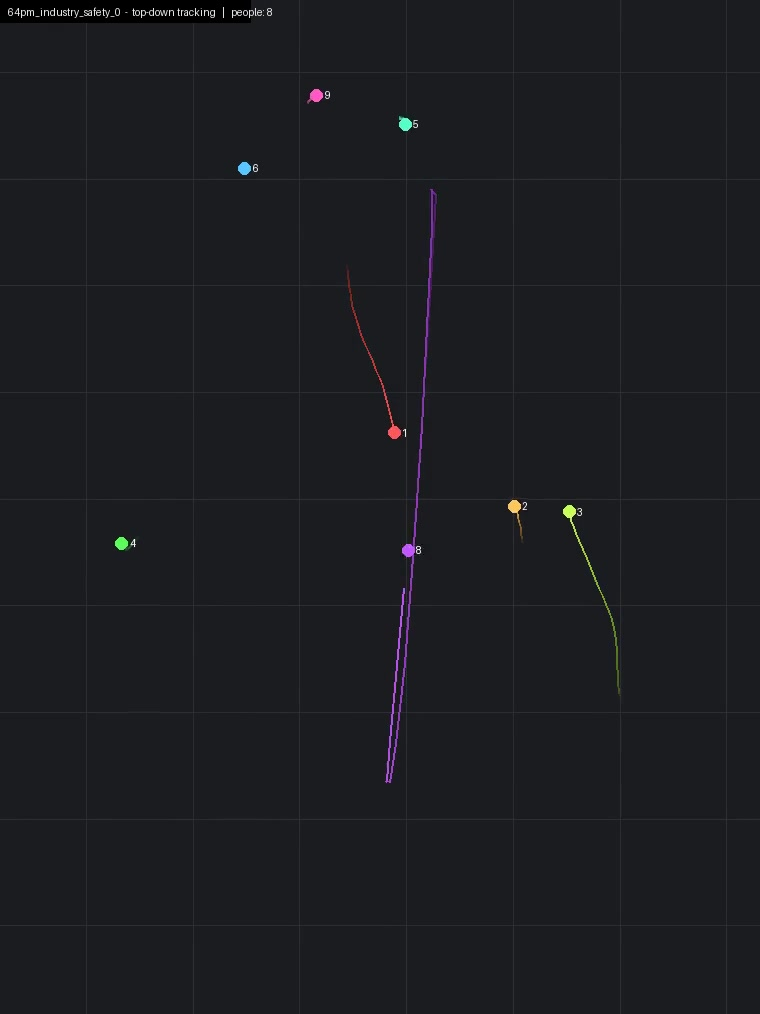
\includegraphics[width=\textwidth]{pipeline_industry_safety_bev}
        \small (d) Industry
    \end{minipage}
    \hfill
    \begin{minipage}[t]{0.48\textwidth}
        \centering
        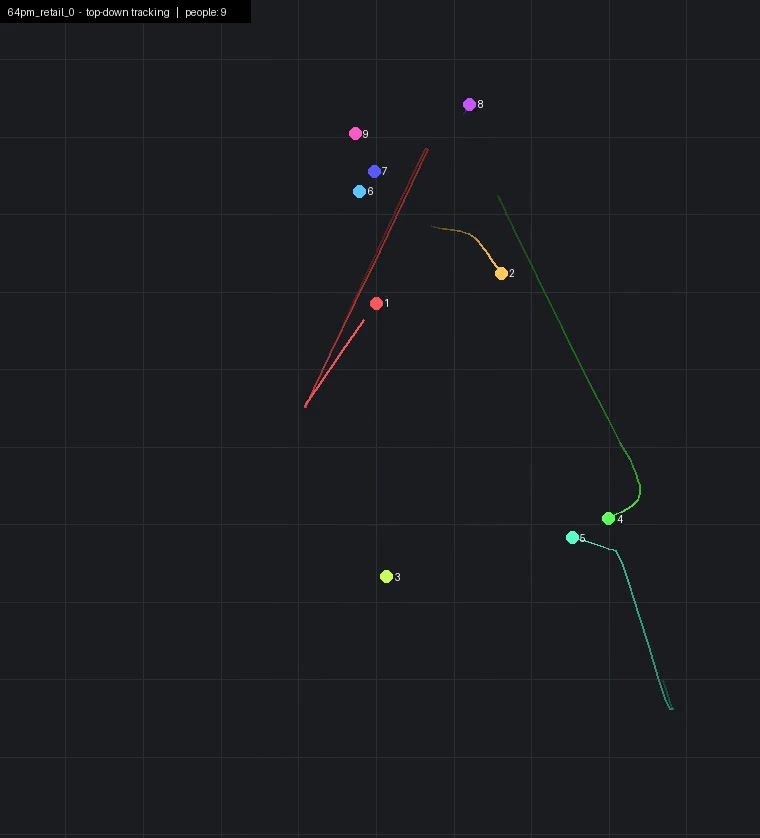
\includegraphics[width=\textwidth]{pipeline_retail_bev}
        \small (e) Retail
    \end{minipage}
    \caption{Góc nhìn BEV trên 5 môi trường}
    \label{fig:pipeline_all_bev}
\end{figure}

\subsection{Thông lượng xử lý}
\label{sec:throughput}

\subsubsection{Thông lượng pipeline production}

Pipeline đầy đủ (YOLO + NvDCF + Swin SGIE + CrossCameraGalleryProbe) với preset mặc định (\texttt{reid0}, \texttt{maxTargetsPerStream=40}) đạt \textbf{$\sim$15 FPS/camera} ở 20 camera đồng thời (3{,}4 GB VRAM) --- vượt mục tiêu 10 FPS/cam. Ảnh hưởng của \texttt{maxTargetsPerStream} lên thông lượng được khảo sát chi tiết ở Bảng~\ref{tab:maxtargets}.

Bottleneck chính được xác định là \textbf{CrossCameraGalleryProbe} (probe tùy chỉnh Python) do giới hạn GIL (Global Interpreter Lock) của Python khi chạy trong GStreamer callback. Vấn đề này được giảm thiểu bằng cách tối ưu hóa vòng lặp matching và cắt giảm số lượng Python object allocation trong hot path.

\subsubsection{Kiểm chứng thông lượng ở 1920$\times$1080 (20 camera)}
\label{sec:throughput_1080p}

Mục tiêu sản phẩm là 20 camera ở 1920$\times$1080 (độ phân giải camera production thực), trong khi tập MMP chỉ 640$\times$360. Để kiểm chứng, pipeline MMP được chạy trên 20 luồng video 1080p của MTMC. Kết quả với được trình bày trong Bảng~\ref{tab:throughput_1080p}.

\begin{table}[H]
    \centering
    \caption[Thông lượng pipeline MMP ở 1080p, 20 camera]{\bfseries\fontsize{12pt}{0pt}\selectfont Thông lượng pipeline MMP trên 20 camera 1920$\times$1080 (video MTMC).}
    \begin{tabular}{|l|c|c|c|c|}
    \hline
    \bfseries Cấu hình & \bfseries Input detector & \bfseries maxTargets & \bfseries VRAM (20 cam) & \bfseries FPS/cam \\
    \hline
    Trên MMPTrack & 640 & 40 & 3,4 GB & $\sim$15 \\
    \textbf{Video 1080p} & 640 & 40 & \textbf{3,83 GB} & \textbf{$\sim$16} \\
    Video 1080p & 960 & 40 & 4,26 GB & $\sim$12 \\
    \hline
    \end{tabular}
    \label{tab:throughput_1080p}
\end{table}

Pipeline MMP (maxTargets=40, input detector 640) trên \textbf{20 camera 1080p thật đạt 3,83 GB / $\sim$16 FPS/cam} --- gần như trùng với số liệu trên dữ liệu MMP gốc (3,4 GB / $\sim$15 FPS/cam), xác nhận pipeline \textbf{giữ vững mục tiêu 20 camera ngay ở độ phân giải 1080p}. Nâng input detector lên 960 giảm còn $\sim$12 FPS/cam; phần VRAM tăng thêm (ví dụ 6,27 GB khi đặt \texttt{maxTargets=100}) là do \texttt{maxTargetsPerStream}, không phải do độ phân giải.

\subsubsection{Sử dụng VRAM}

VRAM được đo trực tiếp bằng \texttt{nvidia-smi} ở trạng thái ổn định trên 20 camera (Bảng~\ref{tab:vram_preset}), thay đổi từng tham số một để cô lập ảnh hưởng. Kết quả cho thấy VRAM bị chi phối chủ yếu bởi \texttt{maxTargetsPerStream}, không phải mô hình ReID nội bộ của NvDCF.

\begin{table}[H]
    \centering
    \caption[Phân rã VRAM theo preset và maxTargetsPerStream]{\bfseries\fontsize{12pt}{0pt}\selectfont VRAM (20 camera, steady-state) theo \texttt{reidType} và \texttt{maxTargetsPerStream}.}
    \begin{tabular}{|l|c|c|c|}
    \hline
    \bfseries Preset & \bfseries \texttt{reidType} & \bfseries \texttt{maxTargets} & \bfseries VRAM (GB) \\
    \hline
    reid0   & 0 & 40  & \textbf{3,4} \\
    reid0   & 0 & 220 & 9,2 \\
    quality & 2 & 40  & 4,2 \\
    quality & 2 & 220 & 12,8 \\
    \hline
    \end{tabular}
    \label{tab:vram_preset}
\end{table}

NvDCF \textbf{cấp phát trước} trạng thái cho từng target (bộ lọc DCF; cộng thêm bộ đệm ReID khi \texttt{reidType:2}) cho toàn bộ sức chứa \texttt{maxTargetsPerStream}~$\times$~số luồng, dù scene thực tế chỉ có 5--15 người/camera. Do đó: (1) riêng việc tăng \texttt{maxTargets} từ 40 lên 220 trên preset reid0 (thêm bộ lọc DCF cho các ô trống, \textit{không liên quan ReID}) đã làm VRAM tăng +5,8 GB; (2) bật mô hình ReID nội bộ chỉ tốn +0,8 GB tại \texttt{maxTargets=40}, nhưng tới +3,6 GB tại \texttt{maxTargets=220} vì bộ đệm ReID cũng được cấp cho mọi ô. Đây là lý do \texttt{maxTargetsPerStream} --- chứ không phải mô hình ReID --- là đòn bẩy VRAM lớn nhất.

Thử nghiệm quantization INT8 không mang lại cải thiện FPS có ý nghĩa (dưới 0{,}5 FPS/cam) trong khi chỉ tiết kiệm $\sim$0{,}37 GB VRAM, nên không được áp dụng trong pipeline production.

\subsubsection{Khảo sát \texttt{maxTargetsPerStream} (FPS và VRAM)}
\label{sec:maxtargets_ablation}

\texttt{maxTargetsPerStream} là số ``ô đối tượng'' (target slot) mà NvDCF \textbf{cấp phát sẵn} cho mỗi luồng camera, bất kể thực tế có bao nhiêu người. Với mỗi ô, NvDCF cập nhật bộ lọc tương quan DCF \emph{mỗi khung}, nên tham số này ảnh hưởng trực tiếp đến cả bộ nhớ lẫn thông lượng. Bảng~\ref{tab:maxtargets} đo trên 20 camera đồng thời với preset \texttt{reid0}, thay đổi từng giá trị một (cửa sổ đo 60 giây ở trạng thái ổn định, lấy mẫu \texttt{nvidia-smi}).

\begin{table}[H]
    \centering
    \caption[Khảo sát maxTargetsPerStream]{\bfseries\fontsize{12pt}{0pt}\selectfont Ảnh hưởng của \texttt{maxTargetsPerStream} đến FPS và VRAM (20 camera, preset reid0).}
    \begin{tabular}{|c|c|c|c|}
    \hline
    \bfseries maxTargetsPerStream & \bfseries FPS/camera & \bfseries FPS tổng & \bfseries VRAM (GB) \\
    \hline
    10  & \textbf{16,50} & 330,0 & \textbf{2,40} \\
    20  & 15,70 & 314,0 & 2,74 \\
    40  & 14,98 & 299,6 & 3,39 \\
    150 & 12,02 & 240,4 & 7,05 \\
    175 & 11,46 & 229,2 & 7,88 \\
    200 & 10,62 & 212,4 & 8,67 \\
    220 & 10,62 & 212,4 & 9,16 \\
    \hline
    \end{tabular}
    \label{tab:maxtargets}
\end{table}

Kết quả cho thấy \texttt{maxTargetsPerStream} là đòn bẩy chi phối: giảm từ 220 xuống 10 giúp \textbf{tăng FPS 55\%} (10,62 $\to$ 16,50 FPS/cam) và \textbf{giảm VRAM 74\%} (9,16 $\to$ 2,40 GB). Ở giá trị mặc định 40, pipeline đạt $\sim$15 FPS/cam với chỉ 3,4 GB VRAM.

Giá trị mặc định production 40 đủ biên an toàn cho scene đông người (mỗi camera MMP có tối đa $\sim$7 người, nhưng NvDCF còn giữ \textit{shadow track} và \textit{tentative track} chiếm thêm ô), để lại $\geq$12 GB dự phòng trên RTX 5060 Ti 16 GB.

\subsection{Hiệu quả của Buffered ID}
\label{sec:buffered_eval}

Bảng~\ref{tab:buffered} so sánh Live ID và Buffered ID trên hai môi trường khó nhất, đo trên \textbf{pipeline hoàn chỉnh đang triển khai} (detector retail-sạch, \texttt{assign\_thr=0,50}). Cột Buffered ID trùng khớp với kết quả theo môi trường trong Bảng~\ref{tab:results}. \textbf{Live ID} = Global ID gán trực tuyến tức thời (cột \texttt{global\_id} thô do CrossCameraGalleryProbe sinh ra); \textbf{Buffered ID} = Global ID anchor-guided sau gom cụm cửa sổ trượt.

\begin{table}[H]
    \centering
    \caption[So sánh Live ID và Buffered ID]{\bfseries\fontsize{12pt}{0pt}\selectfont So sánh Global IDF1: Live ID vs.\ Buffered ID (pipeline triển khai, detector retail-sạch).}
    \begin{tabular}{|l|c|c|}
    \hline
    \bfseries Môi trường & \bfseries Live ID & \bfseries Buffered ID \\
    \hline
    Industry & 0,290 & \textbf{0,847} \\
    Retail   & 0,307 & \textbf{0,661} \\
    \hline
    \end{tabular}
    \label{tab:buffered}
\end{table}

Bảng cho thấy xu hướng rõ rệt: Buffered ID cải thiện Global IDF1 \textbf{2,9 lần} trong môi trường industry (0,290 → 0,847) và \textbf{2,2 lần} trong môi trường retail (0,307 → 0,661). Live ID gán định danh tức thời nên bị ``phình ID'' nghiêm trọng (một người sinh ra hàng chục Global ID khi đi qua nhiều camera/khoảnh khắc che khuất). Kết quả này xác nhận thuật toán anchor-guided \cite{Huang2023} đặc biệt hiệu quả trong môi trường đồng phục, nơi quyết định tức thời của Live ID thường sai nhưng được hiệu chỉnh sau khi tích lũy đủ bằng chứng trong cửa sổ.

Tính trên toàn bộ tập kiểm thử với pipeline hoàn chỉnh, Buffered ID đạt 97--98\% chất lượng của thuật toán offline (xử lý toàn bộ video một lần) với độ trễ chỉ $\sim$20 giây.

\subsubsection{Khảo sát kích thước cửa sổ}
\label{sec:window_ablation}

Để đánh giá ảnh hưởng của kích thước cửa sổ Buffered ID trên toàn tập validation, một thí nghiệm ablation được thực hiện trên đầy đủ 24 scene: pipeline chạy với chunk 100 khung, sau đó thuật toán anchor-guided được áp dụng lại với 4 kích thước cửa sổ (100--400 khung) trên cùng tập embedding. Kết quả Global IDF1 trung bình theo môi trường trình bày trong Bảng~\ref{tab:window_ablation}.

\begin{table}[H]
    \centering
    \caption[Khảo sát kích thước cửa sổ Buffered ID --- toàn tập 24 scene]{\bfseries\fontsize{12pt}{0pt}\selectfont Global IDF1 trung bình theo kích thước cửa sổ Buffered ID (24 scene val).}
    \begin{tabular}{|l|c|c|c|c|}
    \hline
    \bfseries Môi trường & \bfseries \underline{100f} & \bfseries 200f & \bfseries 300f & \bfseries 400f \\
    \hline
    Industry  & 0,847 & 0,836 & 0,841 & \textbf{0,853} \\
    Lobby     & \textbf{0,910} & 0,892 & 0,886 & 0,893 \\
    Office    & \textbf{0,881} & 0,849 & 0,857 & 0,855 \\
    Café      & \textbf{0,844} & 0,829 & 0,820 & 0,823 \\
    Retail    & 0,644 & 0,654 & 0,651 & \textbf{0,657} \\
    \hline
    \textbf{Trung bình} & \textbf{0,794} & 0,785 & 0,784 & 0,789 \\
    \hline
    \end{tabular}
    \label{tab:window_ablation}
\end{table}

(Đo lại với detector retail-sạch đang triển khai, \texttt{assign\_thr=0,50}; các con số nhất quán với
Bảng~\ref{tab:results}.) Khác biệt giữa các kích thước cửa sổ vẫn rất nhỏ (toàn dải chỉ $\sim$0,01
điểm). Cửa sổ \textbf{100 khung} ($\sim$10 giây) đạt trung bình cao nhất (0,794): ba môi trường
lobby/office/café ưa cửa sổ ngắn, trong khi industry và retail nhỉnh hơn ở cửa sổ dài (400 khung) ---
phù hợp trực giác là môi trường đồng phục/che khuất cần tích lũy bằng chứng lâu hơn. Cửa sổ 200 khung
($\sim$20 giây) đang triển khai (0,785 trong khảo sát này; tương ứng 0,798 ở cấu hình chunk-200f của
Bảng~\ref{tab:results}) nằm trong dải nhiễu nên vẫn là lựa chọn hợp lý; có thể hạ xuống 100 khung để
giảm độ trễ một nửa mà gần như không mất chất lượng. Retail ít nhạy cảm nhất với kích thước cửa sổ
(0,644--0,657), một lần nữa xác nhận giới hạn của môi trường này nằm ở \textit{recall phát hiện} (người
bị kệ hàng che khuất), không phải tham số hậu xử lý.

Nếu chọn cửa sổ tối ưu riêng cho từng môi trường (lobby/office/café~=~100f, industry/retail~=~400f) và
tính kết quả oracle tốt nhất trên từng môi trường, trần trên là $\approx$\textbf{0,799} --- ngay sát
ngưỡng 0,800. Điều này xác nhận rào cản còn lại không nằm ở kích thước cửa sổ mà ở recall phát hiện
trong môi trường retail.

\subsection{So sánh kiến trúc mô hình ReID}

Thuật toán anchor-guided clustering được tham khảo từ \cite{Huang2023} sử dụng OSNet làm backbone ReID. Để xác nhận lựa chọn Swin-Tiny thay thế OSNet trong hệ thống này, OSNet-x1.0 (khởi đầu từ pretrain Market-1501 qua torchreid) được huấn luyện trên cùng tập MMP và so sánh trực tiếp:

\begin{table}[H]
    \centering
    \caption[So sánh Swin-Tiny và OSNet trên tập MMP]{\bfseries\fontsize{12pt}{0pt}\selectfont So sánh kiến trúc ReID trên tập val MMPTrack (cross-camera, per-scene)}
    \begin{tabular}{|l|l|c|c|}
    \hline
    \bfseries Mô hình & \bfseries Chuỗi huấn luyện & \bfseries Top-1 & \bfseries mAP \\
    \hline
    \textbf{Swin-Tiny (deployed)} & ImageNet $\to$ MTA $\to$ MMP & \textbf{0{,}853} & \textbf{0{,}784} \\
    OSNet-x1.0 (all)             & Market-1501 $\to$ MMP (70 ids) & 0{,}668 & 0{,}515 \\
    OSNet-x1.0 (no-retail)       & Market-1501 $\to$ MMP (56 ids) & 0{,}610 & 0{,}483 \\
    \hline
    \end{tabular}
    \label{tab:reid_compare}
\end{table}

Swin-Tiny vượt OSNet $\sim$28 điểm phần trăm Top-1. Khoảng cách này phù hợp với xu hướng trong tài liệu ReID: kiến trúc Transformer (Swin) có khả năng mô hình hóa phụ thuộc tầm xa toàn ảnh tốt hơn so với kiến trúc CNN (OSNet), giúp trích xuất đặc trưng phân biệt hơn đặc biệt khi dữ liệu huấn luyện hạn chế như tập MMPTrack. OSNet-noretail tệ hơn OSNet-all ở môi trường retail (0{,}39 vs 0{,}54 Top-1), xác nhận rằng dữ liệu retail phải được giữ trong tập huấn luyện dù tỷ lệ nhãn phantom cao.

Khoảng cách Top-1 có ý nghĩa trực tiếp đến chất lượng pipeline: thuật toán Buffered ID (Anchor-Guided, Phần~\ref{sec:buffered}) phụ thuộc vào độ chính xác của các ``tracklet anchor'' --- tracklet có embedding ổn định đủ để đại diện cho một người xuyên camera. Embedding OSNet yếu hơn dẫn đến anchor kém phân biệt hơn, làm tăng khả năng gộp nhầm hai người khác nhau vào cùng Global ID trong bước clustering.

\textbf{Kết luận:} Giữ nguyên \textbf{Swin-Tiny} làm mô hình deployed trên tập MMPTrack.

\subsection{Trực quan hoá pipeline trên MTMC (Warehouse\_022)}
\label{sec:mtmc_results}

Pipeline được chạy thử trên bộ dữ liệu thứ hai MTMC (Phần~\ref{sec:mtmc_dataset}), giới hạn ở kho Warehouse\_022. Bối cảnh kho có hiệu chỉnh metric thuận lợi cho việc trực quan hoá các chức năng phân tích (heatmap, quỹ đạo theo dõi trên bản đồ BEV chung); và khi chạy pipeline ở đây, một số hạn chế của phương pháp khi chuyển sang mạng camera rời rạc cũng bộc lộ rõ. Do dữ liệu là mô phỏng, đây là phép trực quan hoá chức năng chứ không phải một benchmark định lượng. Detector YOLO11n và mạng ReID Swin được huấn luyện lại trên dữ liệu kho (tách biệt với mô hình MMP), còn tracker NvDCF dùng \texttt{maxTargetsPerStream} cao hơn cho mật độ kho.

Điểm khác biệt cốt lõi nằm ở khâu hợp nhất định danh xuyên camera. Trên MMP (camera chồng lắp), Global ID được tạo dựa trên ngoại hình (anchor-guided clustering); nhưng trên MTMC cách này chỉ đạt Global IDF1 khoảng 0,29, vì các camera rời rạc và crop người trong kho nhỏ, bị che nên embedding của các danh tính khác nhau không tách bạch. Khi thay bằng nối định danh theo vị trí thế giới --- chiếu điểm chân của mỗi người xuống mặt sàn qua calibration metric rồi gom cụm có ràng buộc không-thời gian --- Global IDF1 tăng lên khoảng 0,86 (xấp xỉ 92\% trần lý thuyết 0,93). Do cùng một bộ mô hình và chỉ thay phương pháp nối, chênh lệch này đến từ thuật toán hợp nhất chứ không phải chất lượng mô hình.

Các chức năng phân tích vùng tuỳ biến (vùng ROI, vạch đếm, cảnh báo quá tải, vùng cấm) cấu hình qua ROI editor của Web UI cũng hoạt động bình thường trên bối cảnh kho hàng (Hình~\ref{fig:w022_analytics}).

\begin{figure}[H]
    \centering
    \begin{minipage}[t]{0.32\textwidth}
        \centering
        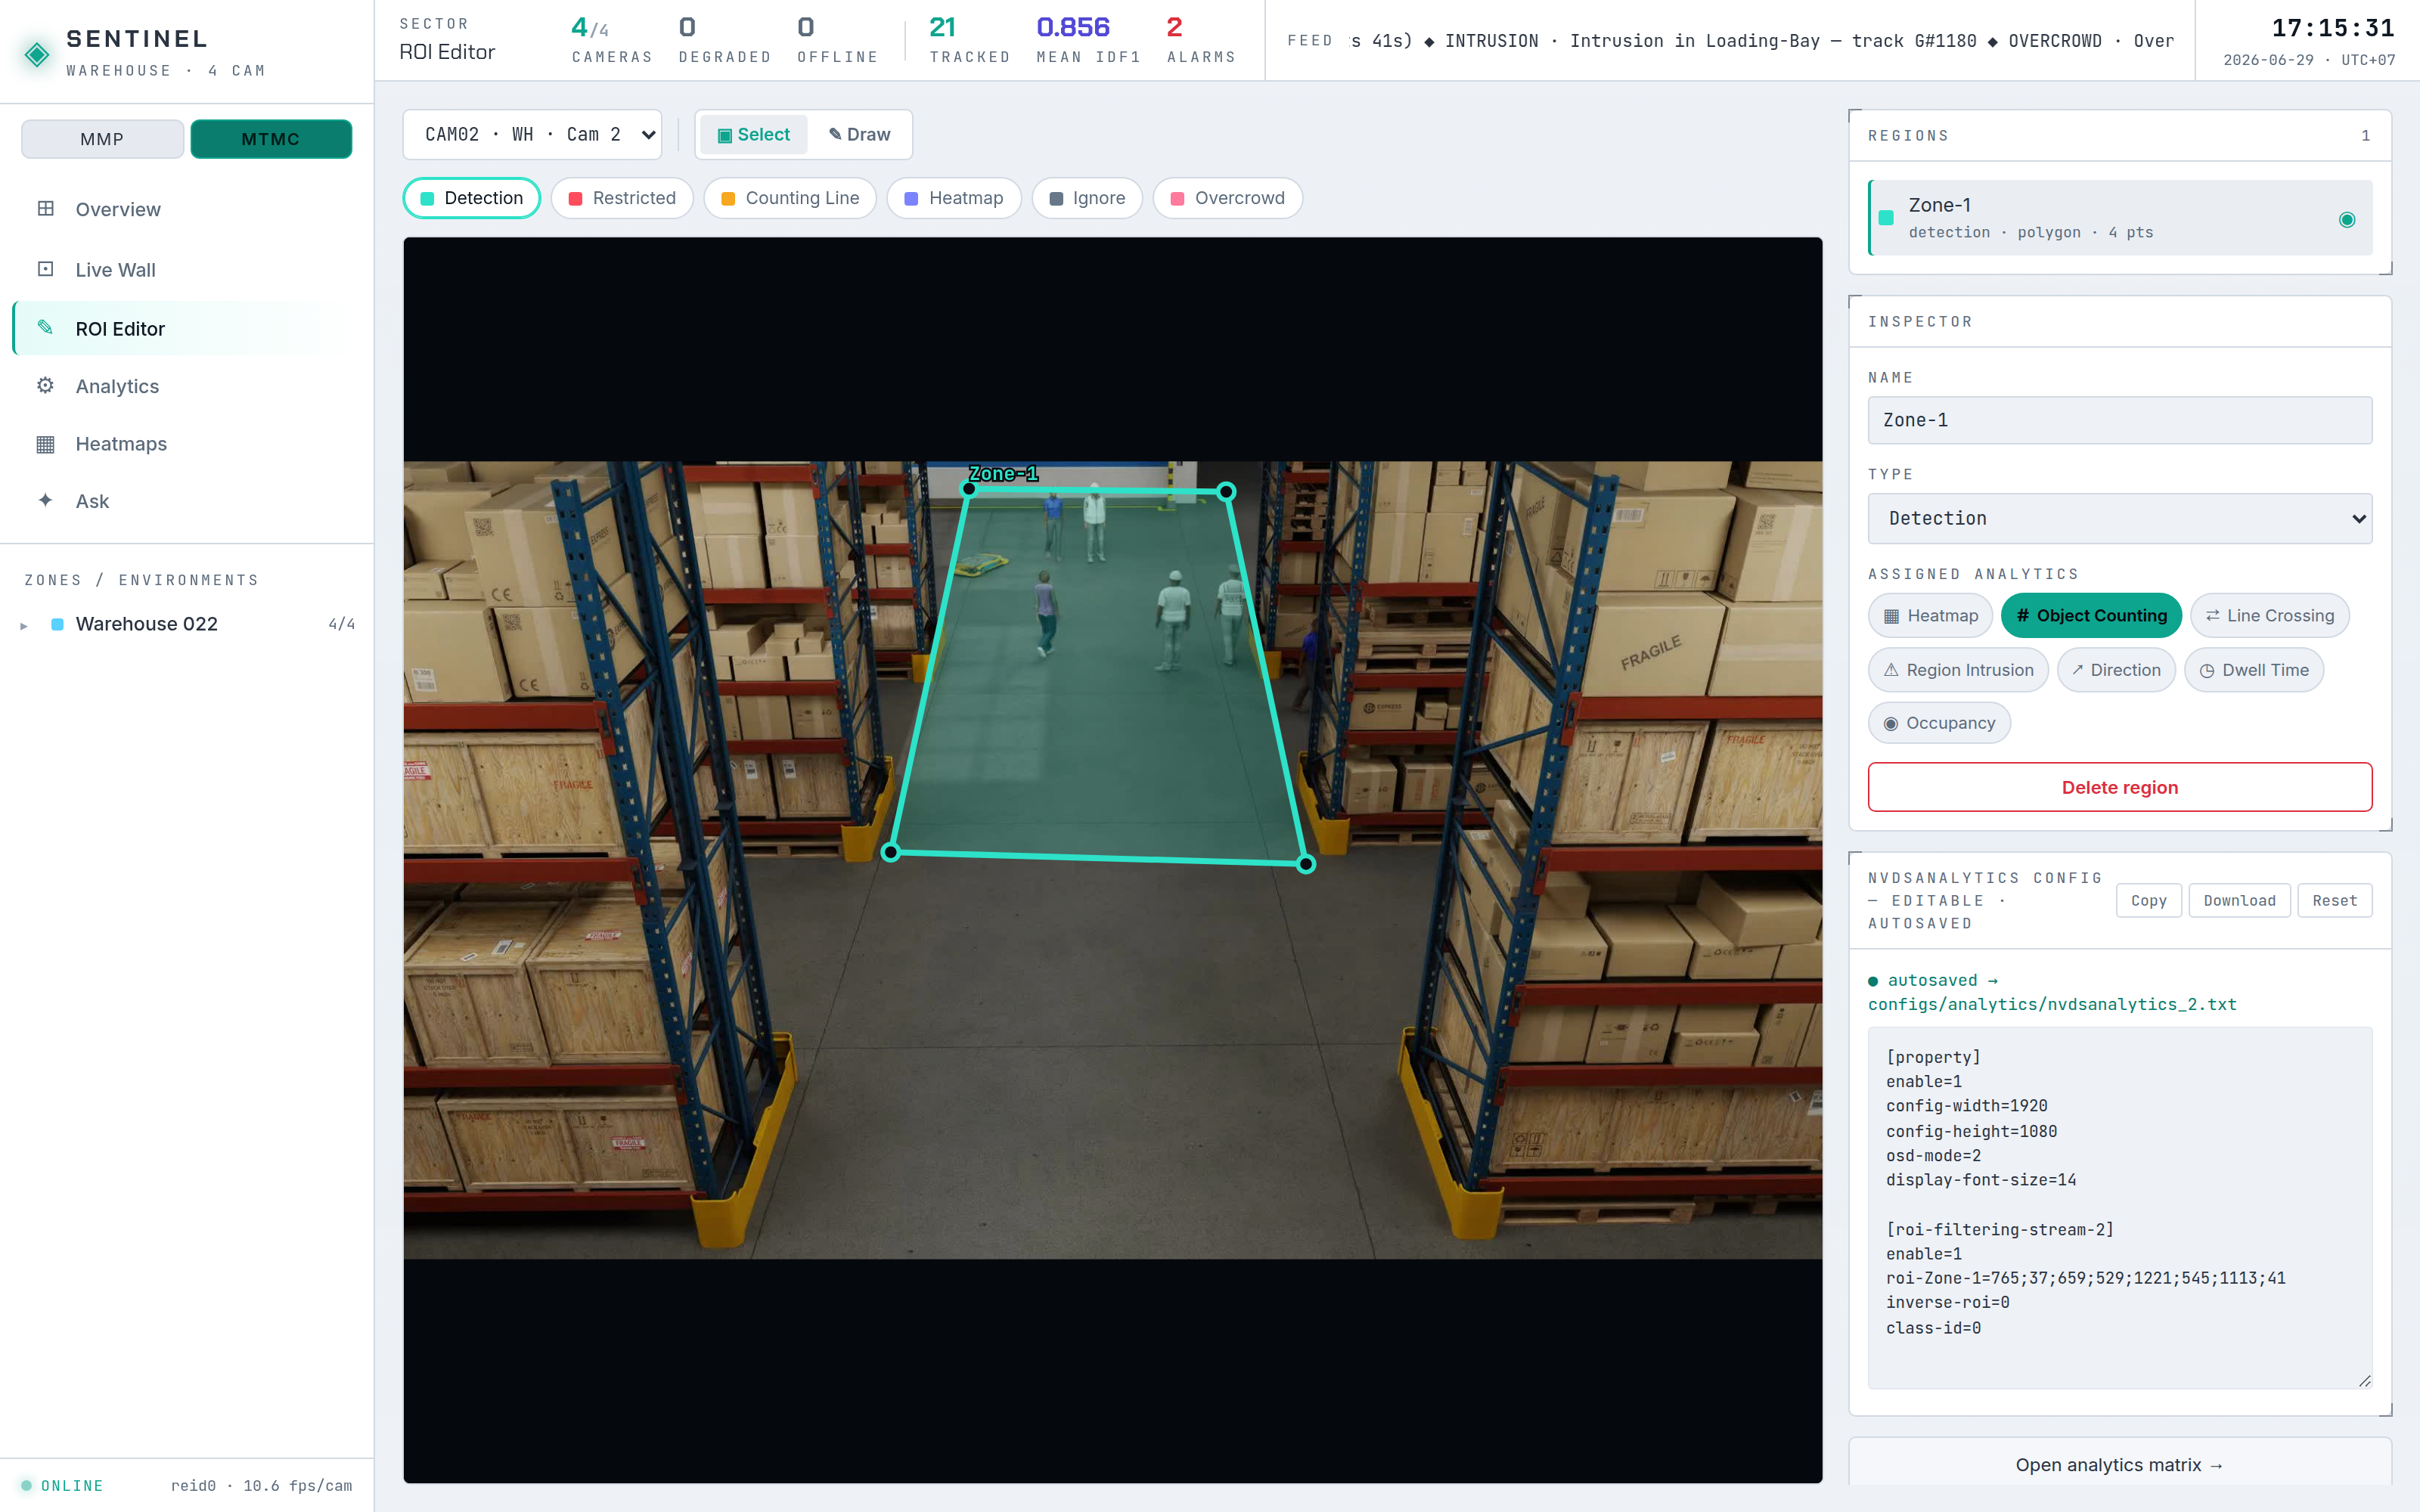
\includegraphics[width=\textwidth]{webui_roi_w022_zone}
        \small (a) Vùng ROI
    \end{minipage}
    \hfill
    \begin{minipage}[t]{0.32\textwidth}
        \centering
        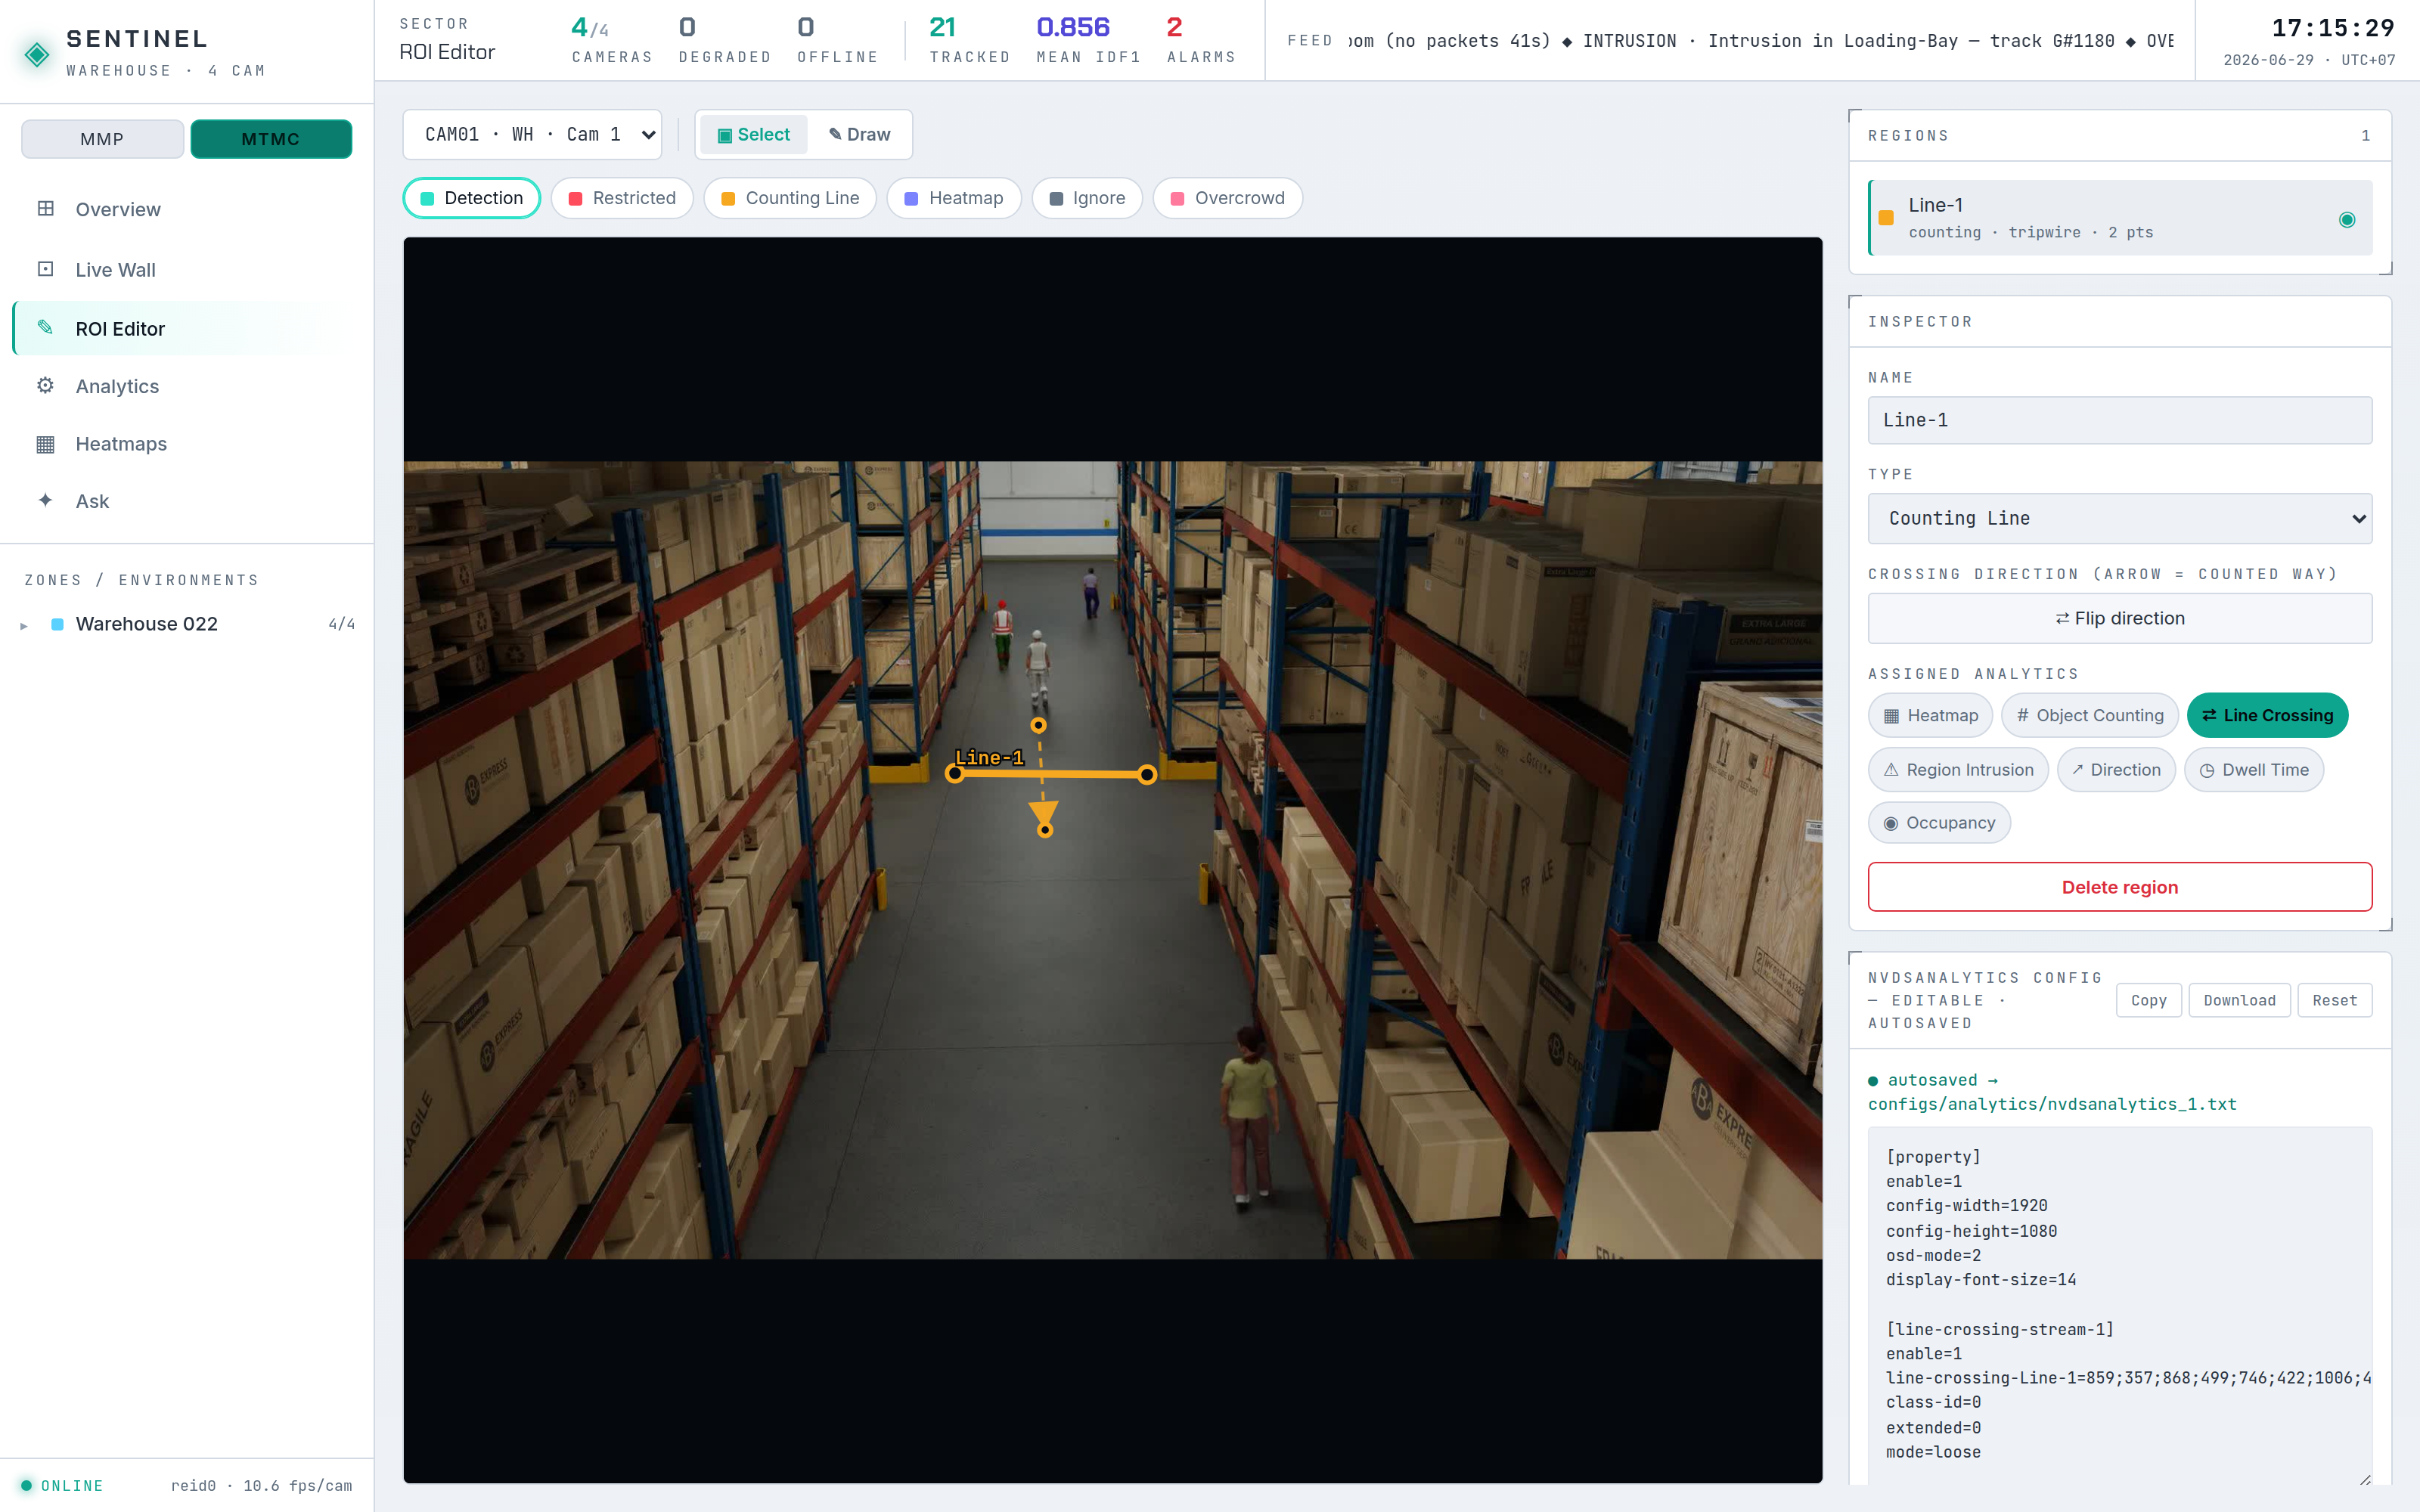
\includegraphics[width=\textwidth]{webui_roi_w022_linecross}
        \small (b) Line-crossing
    \end{minipage}
    \hfill
    \begin{minipage}[t]{0.32\textwidth}
        \centering
        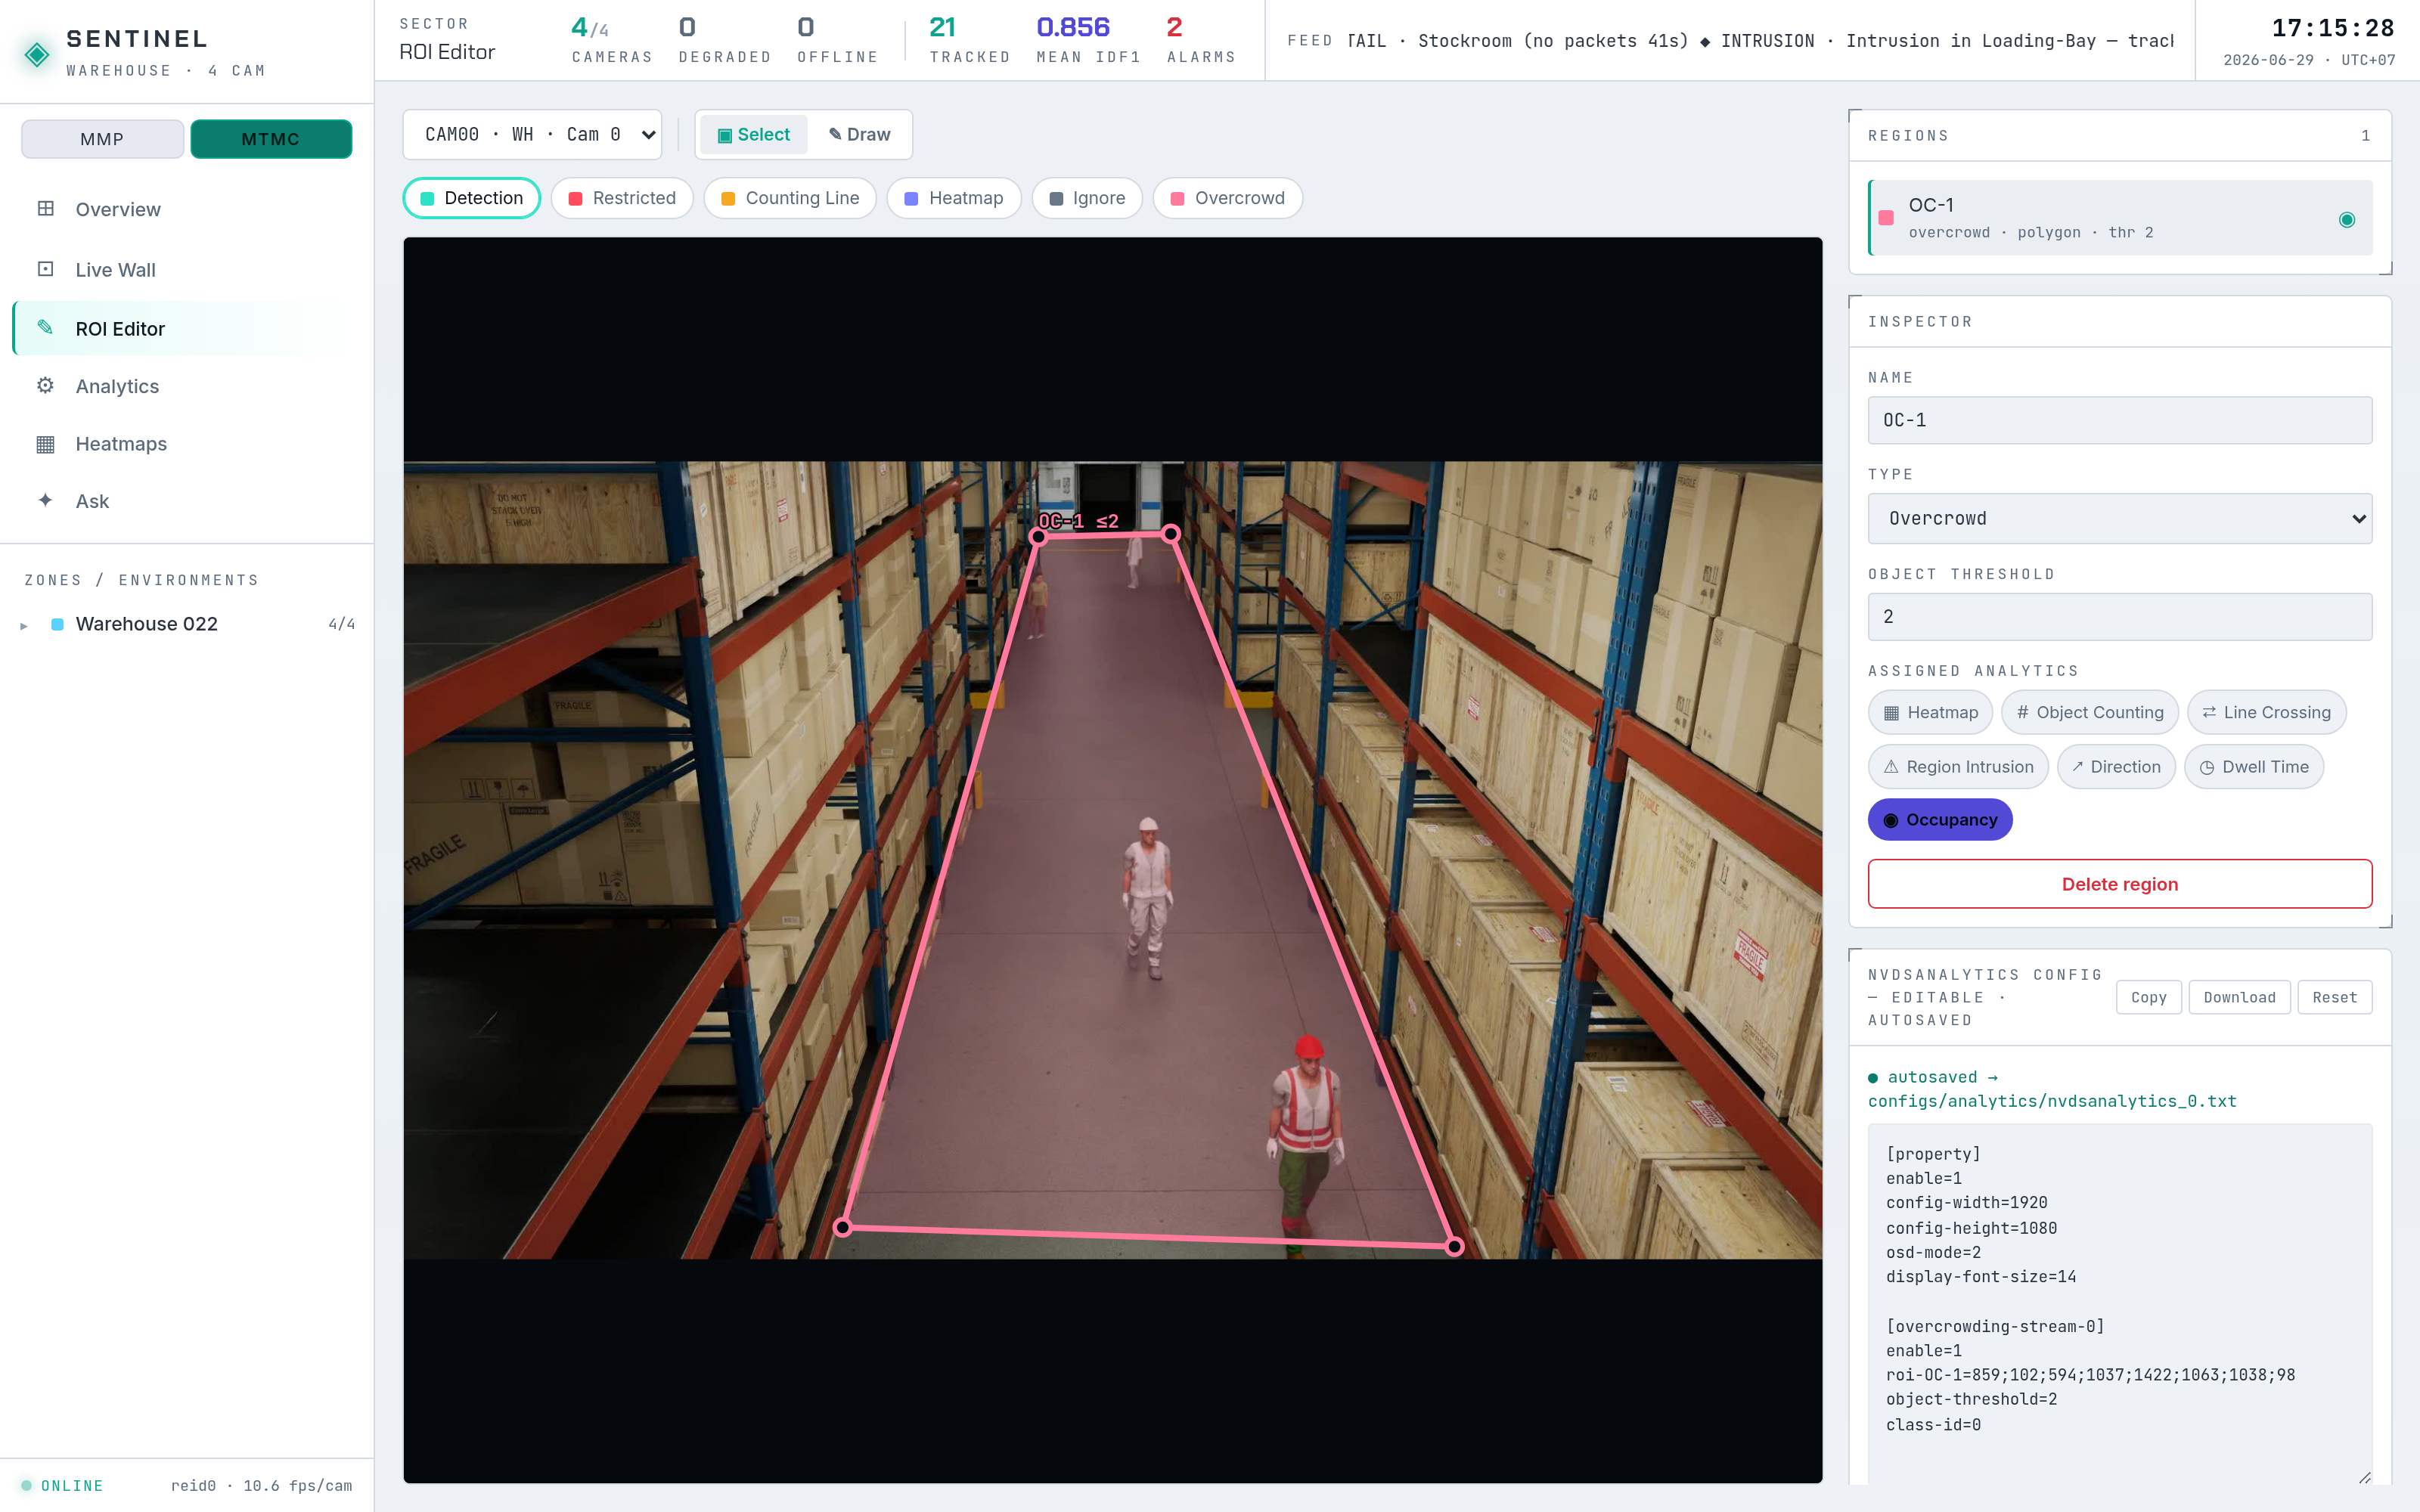
\includegraphics[width=\textwidth]{webui_roi_w022_overcrowd}
        \small (c) Overcrowding
    \end{minipage}
    \\[6pt]
    \begin{minipage}[t]{0.48\textwidth}
        \centering
        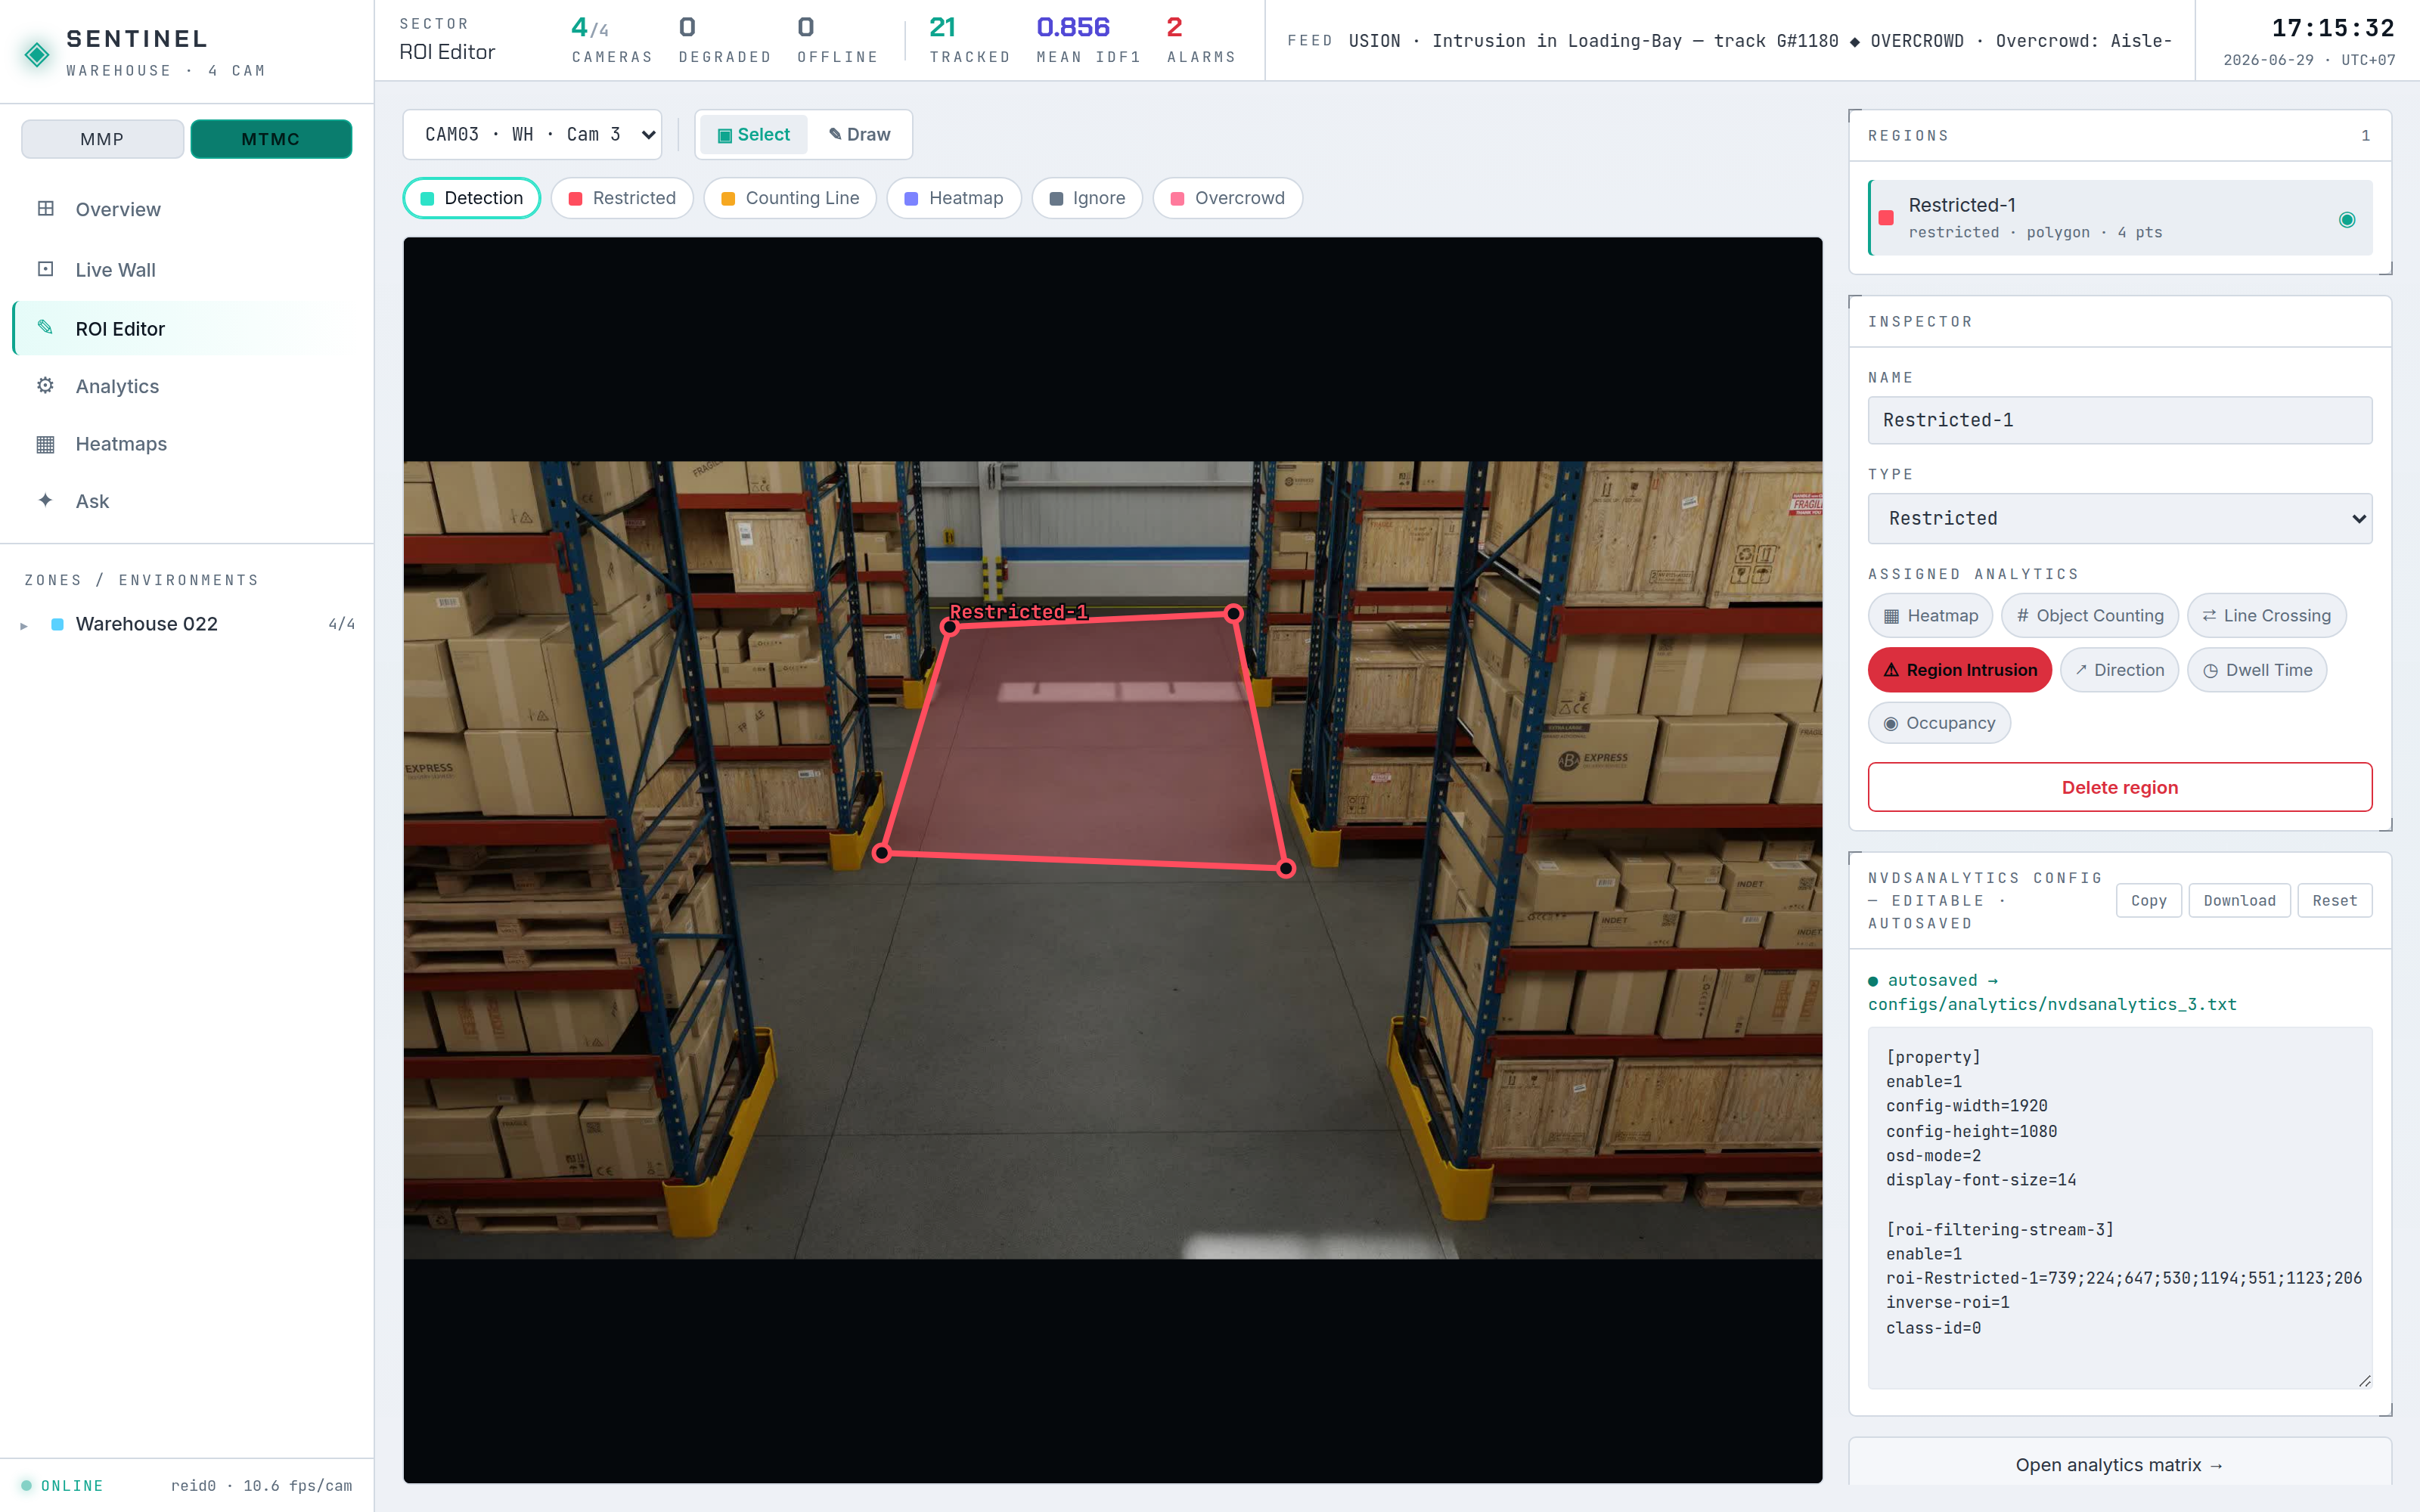
\includegraphics[width=\textwidth]{webui_roi_w022_restricted}
        \small (d) Vùng cấm (restricted)
    \end{minipage}
    \hfill
    \begin{minipage}[t]{0.48\textwidth}
        \centering
        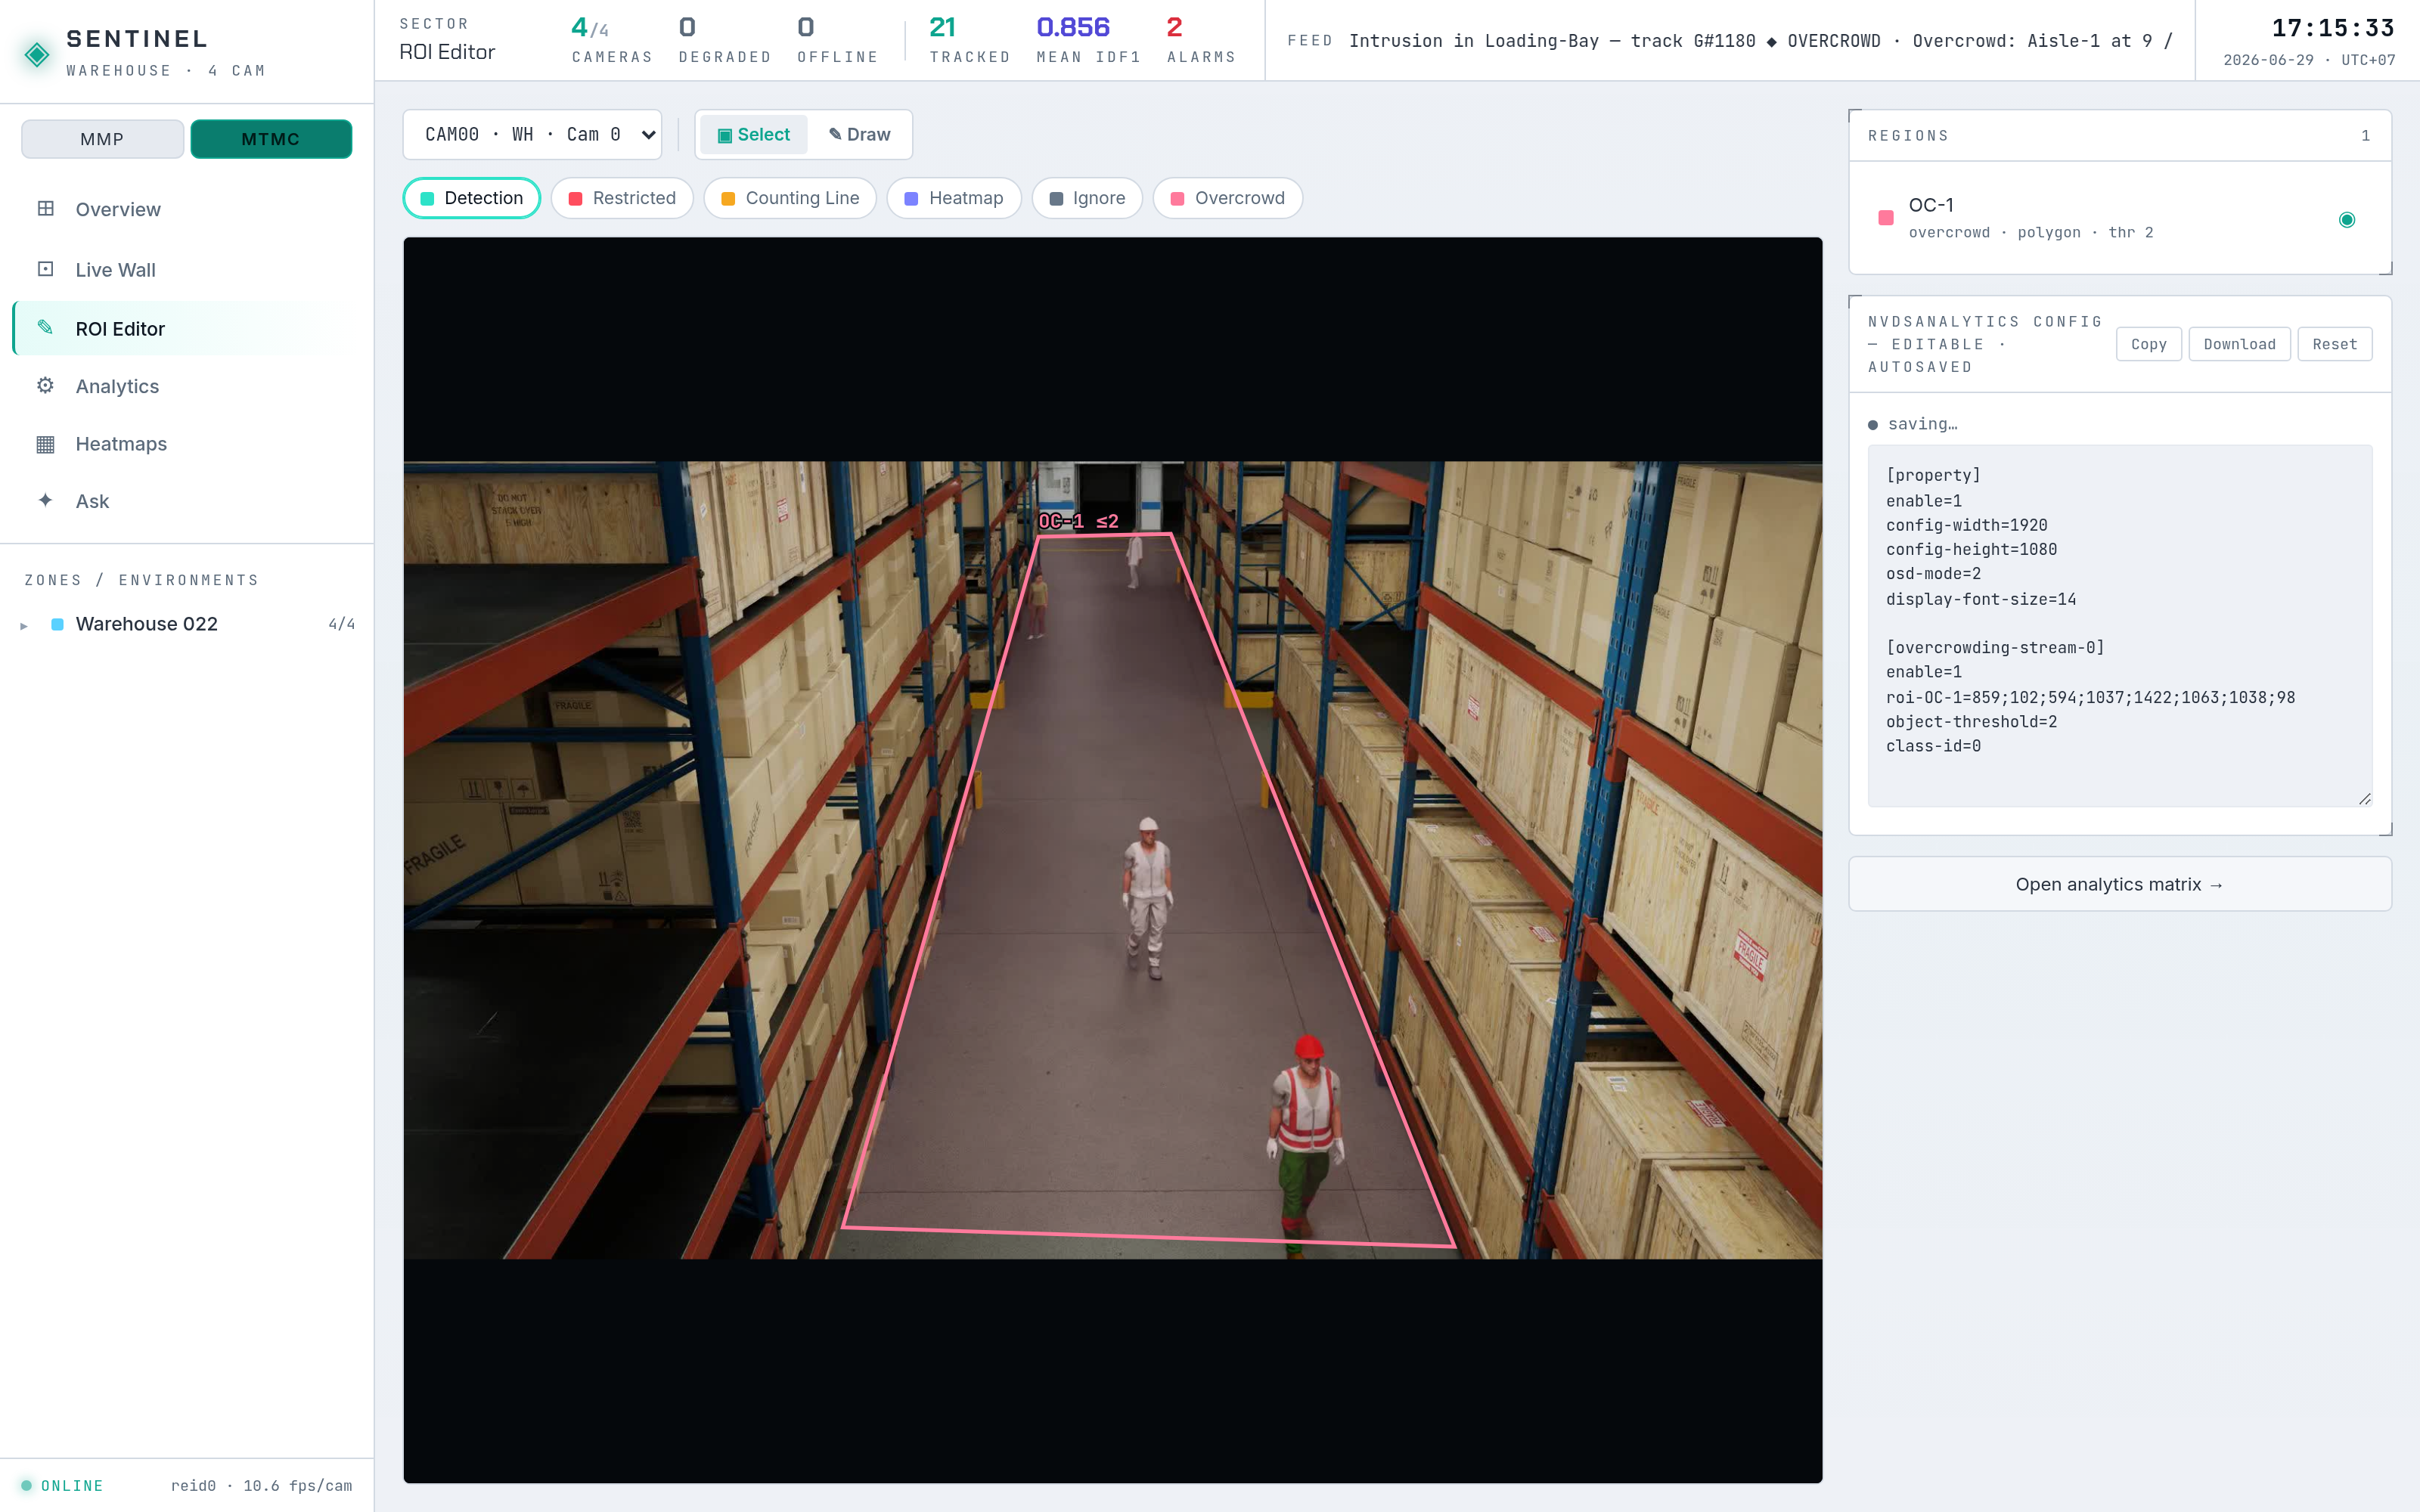
\includegraphics[width=\textwidth]{webui_custom_analytics_w022}
        \small (e) Bảng phân tích tuỳ biến
    \end{minipage}
    \caption{Phân tích vùng tuỳ biến trên kho hàng Warehouse\_022, cấu hình qua ROI editor của Web UI.}
    \label{fig:w022_analytics}
\end{figure}

Hai hạn chế chính rút ra từ MTMC:
\begin{itemize}
    \item Khâu hợp nhất theo ngoại hình (thiết kế cho FOV chồng lắp của MMP) không tổng quát sang mạng camera rời rạc; ở đó cần ưu tiên vị trí hình học và do đó cần calibration metric. Pipeline chưa tự động chuyển chế độ mà phải chọn phương pháp nối phù hợp với loại mạng camera.
    \item Recall phát hiện dưới che khuất là trần cứng: góc camera nông và lối đi dài làm nhiều người bị che ở mọi góc nhìn cùng lúc, nên ngay cả khi định danh hoàn hảo, IDF1 cũng chỉ đạt khoảng 0,93. Tăng độ phân giải gần như không cải thiện vì nút thắt là che khuất, không phải độ phân giải.
\end{itemize}

\newpage

%%%%%%%%%%%%%%%%%%%%%%%%%%%%%%%%%%%%%%%%%%%%%%%%%%
%               KẾT LUẬN
%%%%%%%%%%%%%%%%%%%%%%%%%%%%%%%%%%%%%%%%%%%%%%%%%%
\section*{KẾT LUẬN}
\phantomsection\addcontentsline{toc}{section}{\numberline {}KẾT LUẬN}

\subsection*{Kết luận chung}
\phantomsection\addcontentsline{toc}{section}{\numberline {}Kết luận chung}

Dự án đã xây dựng thành công hệ thống theo dõi người đa camera theo thời gian thực:

\begin{itemize}
    \item \textbf{Thông lượng:} $\sim$15 FPS/camera tại 20 camera đồng thời (preset reid0, maxTargetsPerStream=40), vượt mục tiêu 10 FPS/cam.
    \item \textbf{Độ chính xác:} Global IDF1 trung bình 0,798 trên đầy đủ 24 cảnh validation với người unseen; bốn trong năm môi trường (lobby, office, industry, café) đều vượt ngưỡng mục tiêu 0,8.
\end{itemize}

Ba đóng góp kỹ thuật quan trọng giúp đạt được các kết quả trên là: (1) quy trình làm sạch nhãn loại bỏ nhiễu đáng kể trong dữ liệu MMPTrack; (2) huấn luyện lại detector trên nhãn retail đã làm sạch, loại bỏ Phantom Groundtruth trong scene retail (precision 0,62 $\to$ 0,94) và nâng Global IDF1 toàn tập từ 0,774 lên 0,798; (3) triển khai Buffered ID dựa trên anchor-guided clustering \cite{Huang2023} trong cửa sổ trượt 20 giây, giúp cải thiện Global IDF1 từ 0,290 lên 0,847 trong môi trường khó (industry đồng phục).

Bên cạnh theo dõi, hệ thống còn cung cấp bộ công cụ phân tích không gian (heatmap Occupancy, Footfall, Dwell-time), sẵn sàng tích hợp vào các ứng dụng giám sát an toàn, tối ưu không gian và phân tích lưu lượng người.

\subsection*{Hạn chế}
\phantomsection\addcontentsline{toc}{section}{\numberline {}Hạn chế}

Hệ thống còn một số hạn chế cần ghi nhận:

\begin{itemize}
    \item \textbf{Môi trường retail:} Global IDF1 chỉ đạt 0,661, thấp hơn đáng kể so với các môi trường khác. Sau khi huấn luyện lại detector trên nhãn sạch đã loại phần lớn phát hiện ``ma'', nguyên nhân còn lại là che khuất do kệ hàng làm detector bỏ sót người thực (giảm recall) --- giới hạn vật lý của camera CCTV thông thường không thể giải quyết hoàn toàn bằng thuật toán.

    \item \textbf{Đồng phục:} Trong môi trường industry và retail, người mặc đồng phục giống nhau gây khó khăn cho mô hình ReID, dẫn đến nhầm lẫn định danh.

    \item \textbf{Độ trễ Buffered ID:} Chế độ Buffered ID giới thiệu độ trễ $\sim$20 giây. Trong ứng dụng yêu cầu định danh tức thời (như mở cửa theo người), cần sử dụng Live ID với chất lượng thấp hơn.

    \item \textbf{Phụ thuộc hiệu chỉnh camera:} Ràng buộc hình học yêu cầu ma trận homography calibration cho từng camera. Nếu camera bị di chuyển, cần hiệu chỉnh lại.
\end{itemize}

\subsection*{Hướng phát triển}
\phantomsection\addcontentsline{toc}{section}{\numberline {}Hướng phát triển}

Các hướng phát triển tiếp theo:

\begin{itemize}
    \item \textbf{Cải thiện ReID cho đồng phục:} Khám phá đặc trưng dáng đi (gait features) hoặc đặc trưng từ ảnh nhiệt hồng ngoại để phân biệt người trong môi trường đồng phục.

    \item \textbf{Mở rộng sang camera RTSP:} Kiểm thử pipeline với luồng RTSP từ camera thực tế (hiện tại chỉ kiểm thử với file video).

    \item \textbf{Tích hợp mô hình BEV:} Nghiên cứu khả năng tích hợp MCBLT \cite{Wang24MCBLT} hoặc phương pháp BEV tương tự vào pipeline, hoặc sử dụng như post-processing layer để cải thiện định danh trong các scene khó.

    \item \textbf{Giảm độ trễ Buffered ID:} Nghiên cứu thuật toán online clustering có khả năng ra quyết định sớm hơn trong cửa sổ, giảm độ trễ xuống dưới 10 giây mà không làm giảm đáng kể chất lượng.

\end{itemize}

\newpage
\phantomsection\addcontentsline{toc}{section}{\numberline {}TÀI LIỆU THAM KHẢO}
\bibliographystyle{IEEEtran}
\bibliography{MyRef}
\newpage
\section*{PHỤ LỤC}
\phantomsection\addcontentsline{toc}{section}{\numberline{} PHỤ LỤC}

\subsection*{A. Tài nguyên dự án}

\begin{itemize}
    \item \textbf{Mã nguồn (GitHub):}
    \url{https://github.com/NLT22/multi\_stream\_people\_tracker}

    \item \textbf{Video demo và hình ảnh (Google Drive):}
    \url{https://drive.google.com/drive/folders/1yO3T-kCAQ-KZG0K4Tydum4X66aGpdzhx?usp=sharing}
\end{itemize}

\subsection*{B. Cấu trúc thư mục demo}

Thư mục demo được tổ chức theo từng môi trường. Mỗi môi trường có một bộ đầy đủ gồm 3 video và thư mục heatmap:

\begin{center}
\texttt{output/demo/<môi-trường>/}
\end{center}

\begin{table}[H]
\centering
\begin{tabular}{|l|p{10cm}|}
\hline
\bfseries File & \bfseries Nội dung \\
\hline
\texttt{<env>\_live\_buffered\_osd.mp4} & 4 camera đồng thời, hiển thị Buffered ID ổn định + quỹ đạo di chuyển \\
\texttt{<env>\_tracking\_bev.mp4}       & Góc nhìn từ trên xuống (BEV): mỗi người một chấm màu + vệt đường đi \\
\texttt{<env>\_analytics.mp4}           & ROI đếm người + cảnh báo quá tải + vạch đếm vào/ra (cấu hình riêng từng môi trường) \\
\texttt{heatmap/}                       & 15 ảnh PNG: \texttt{cam\_\{0--3\}\_\{typeheatmap\}.png} và \texttt{bev\_\{typeheatmap\}.png} \\
\hline
\end{tabular}
\end{table}

Năm môi trường: \texttt{office}, \texttt{cafe\_shop}, \texttt{lobby}, \texttt{industry\_safety}, \texttt{retail}. Tất cả video sử dụng chế độ \textbf{Buffered ID (anchor-guided)} để hiển thị định danh ổn định.
 % Phụ lục nếu có
\end{document}
